\chapter{Análisis Exploratorio de Datos}

Un análisis exploratorio se realiza para una investigacion y entendimiento afondo de los datos, y asi descubrir patrones ocultos y generar hipótesis, a traves de tecnicas de visualización de datos, análisis de correlación o minería de datos.\\

El propósito de este análisis es identificar características diferenciadoras entre los microbiomas de plantas sanas y enfermas mediante el uso de datos metagenómicos. Para llevar a cabo este estudio, se obtuvieron datos metagenómicos de la empresa Solena, específicamente de microorganismos presentes en cultivos de fresa. Inicialmente, se dividieron las muestras en dos poblaciones: aquellas etiquetadas como $"$sanas$"$ y $"$enfermas$"$.\\

En una primera etapa, se llevó a cabo un exhaustivo preprocesamiento de los datos, utilizando los lenguajes de programación, BASH y R. Posteriormente, se inició el análisis exploratorio de datos, el cual se estructura principalmente en tres partes. En primer lugar, se realizó una exploración que abarcó las diversidades alfa y beta. Esto condujo a un análisis estadístico respaldado por pruebas de hipótesis. En segundo lugar, se llevó a cabo una visualización de correlaciones mediante redes.\\ %Por último, se implementó una clasificación empleando técnicas de machine learning.\\

Este enfoque integral no solo proporciona una comprensión detallada de la composición de los microbiomas en las plantas de fresa, sino que también permite identificar patrones significativos que podrían ser fundamentales para distinguir entre la salud y la enfermedad en estos cultivos (\cite{yang2020}). 
Este enfoque integral no solo proporciona una comprensión detallada de la composición de los microbiomas en las plantas de fresa, sino que también permite identificar patrones significativos en las diferencias ya sea de presencia-ausencia o abundancia de microorganismos, que podrían ser fundamentales para distinguir entre la salud y la enfermedad en estos cultivos.

\section{Preprocesamiento}

Dentro de las etapas principales de los datos, se encuentra la adquisición de los datos, en donde se recopilan los datos necesarios para el análisis. Se ha adquirido un conjunto de datos metagenómicos de cultivos de fresa proporcionados por Solena. Estas secuencias se entregaron en formato fasta y se encuentran almacenadas en archivos Json, siendo el resultado de la clasificación metagenómica realizada mediante el clasificador Kraken. Con la finalidad de identificar características distintivas entre los frutos sanos y enfermos, hemos llevado a cabo un análisis exploratorio de estos datos.\\

\begin{figure}[h]
\centering
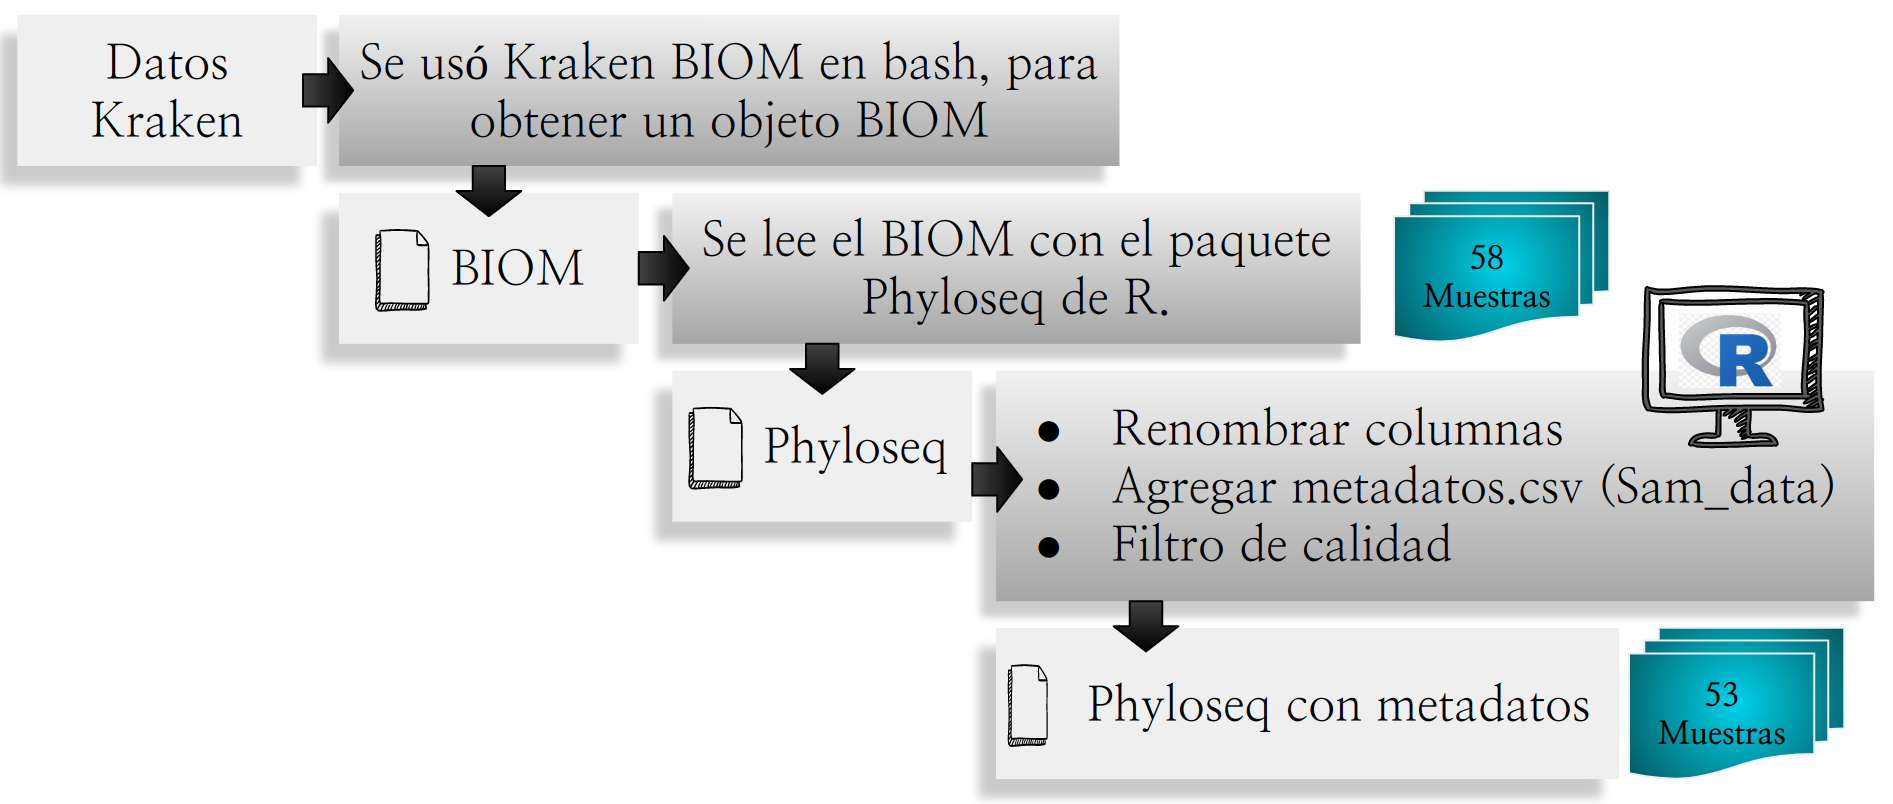
\includegraphics[width=\textwidth]{Img/cap2/preprosecamiento.png}
\caption{Flujo de trabajo, preprocesamiento de datos}
\end{figure}

Dentro de este preprocesamiento es necesario realizar una limpieza y trasformación de los datos para que estos sean adecuados para el análisis. En este caso se realizó un cambio de formato a objeto BIOM, para un mejor manejo de los datos; luego fue necesario renombrar columnas, agregar los metadatos y realizar un filtro de calidad, que se explicara a fondo más adelante.\\

\subsection{Phyloseq}

Phyloseq es un Software de Código Abierto para Bioinformática (Open Source Software For Bioinformatics), diseñado para la manipulación y análisis integral de datos metagenómicos generados mediante tecnologías de secuenciación de alto rendimiento. Esta herramienta en R ofrece capacidades para importar, almacenar, analizar y visualizar datos metagenómicos de manera eficiente. En el entorno de R, estos datos se estructuran en un objeto Phyloseq, el cual tiene la versatilidad de contener elementos clave, como la tabla de taxonomía, la tabla de conteos, la tabla de muestras o metadatos, y el árbol filogenético. Esta organización multifacética facilita un análisis completo y preciso de la estructura de la comunidad microbiana, brindando una comprensión profunda de los datos metagenómicos en cuestión. (\cite{mcmurdie2013})\\

\begin{figure}[h]
\centering
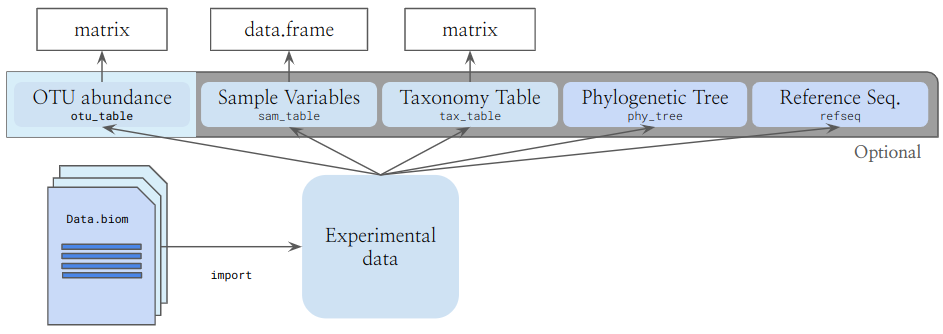
\includegraphics[width=\textwidth]{Img/cap2/Phyloseq.png}
\caption{Objeto phyloseq }%\citep{Introducción a phyloseq-castrolab})}
\end{figure}

Para iniciar el análisis de estos datos, llevamos a cabo una exploración general utilizando índices ecológicos, especialmente centrándonos en las diversidades alfa y beta. Importamos los datos como un objeto Phyloseq, que puede incluir cuatro componentes: la matriz de abundancias, la tabla de taxonomía, los metadatos y el árbol filogenético. Este enfoque nos permite obtener una comprensión más profunda de la estructura de la comunidad microbiana presente en los datos metagenómicos, empleando medidas de diversidad para evaluar la variabilidad intra e inter-muestral.

\subsection{Filtrado de Calidad}

Después de realizar una revisión inicial de los datos, notamos la presencia de muestras con conteos de ceros (número de lecturas por muestras), como en el caso de 'MP2088'. A través de Solena, obtuvimos una tabla que refleja la calidad de las muestras (fastp.kraken.summary \href{https://github.com/CamilaSilva1995/Tesis_Maestria/blob/main/Analisis_Comparativo/Fresa_Solena/01_Exploracion.pdf}). Esta información es crucial para determinar qué muestras pueden ser eliminadas de nuestro conjunto de datos, ya que no cumplen con ciertos estándares de calidad. La identificación y exclusión de muestras que no cumplen con estos criterios contribuirá a asegurar la integridad y la confiabilidad de nuestro dataset, garantizando que solo las muestras de alta calidad sean consideradas en el análisis subsiguiente.\\

Esta tabla proporciona información detallada sobre la calidad de las muestras, destacando diversos parámetros clave:
\begin{itemize}
  \item \textbf{ID de la muestra:} Identificación única de la muestra.
  \item \textbf{Reads\_B  (Reads\_Before):} Número total de lecturas crudas antes del análisis de calidad.
  \item \textbf{Reads\_A (Reads\_After):} Número total de lecturas después del análisis de calidad.
  \item \textbf{Reads\_diff:}  Diferencia entre Reads\_B y Reads\_A.
  \item \textbf{Q30\_B:} Porcentaje de lecturas con calidad superior a 30 (escala fred) antes del análisis de calidad.
  \item \textbf{Q30\_A:} Porcentaje de lecturas con calidad superior a 30 después del análisis de calidad.
  \item \textbf{LowQua:} Lecturas de baja calidad.
  \item \textbf{N\_reads:} Lecturas que contienen 'N' y son descartadas.
  \item \textbf{too\_short:}  Lecturas que no cumplen con el tamaño mínimo de calidad.
  \item \textbf{Duplication:} Porcentaje de duplicados.
  \item \textbf{LengthR1:} Longitud promedio de las lecturas en la muestra.
  \item \textbf{LengthR2:} Longitud promedio de las lecturas en la muestra.
  \item \textbf{Classified:} Porcentaje de lecturas clasificadas del total después del filtrado.
\end{itemize}

Como ejemplo, la muestra MD2055 inicialmente tiene 97 millones de lecturas antes del filtrado, y después del análisis de calidad queda con 79 millones. El criterio para eliminar muestras es que, después del filtrado de calidad, contengan menos de 25 millones de lecturas. Bajo este filtro, se identificaron y eliminaron cinco muestras: MP2079, MP2080, MP2088, MP2109, MP2137.\\

Eliminamos las muestras de baja calidad, usando el filtro de menos de 25 millones de lecturas luego del análisis de calidad.\\

Este enfoque de eliminación se basa en mantener un umbral mínimo de calidad, contribuyendo así a garantizar la robustez y confiabilidad de las muestras seleccionadas para análisis subsiguientes. Además, se puede realizar un recuento de lecturas por muestra para evaluar la calidad relativa entre las diferentes muestras,\\

\begin{lstlisting}[basicstyle=\small] 
sample_sums(fresa_kraken)
\end{lstlisting}
\resizebox{0.9\textwidth}{!} {
\begin{tabular}{ c c c c c c c c }
MD2055 & MD2056 & MD2065 & MD2066 & MD2075 & MD2076 & MD2085 & MD2086 \\
9782432 & 12468526 & 11297600 & 15580959 & 12310781 & 16067839 & 10524919 & 9931297 \\
MD2095 & MD2096 & MD2105 & MD2106 & MD2115 & MD2116 & MD2125 & MD2126 \\
18009912 & 14998268 & 11792397 & 4053295 & 13102554 & 12451637 & 8355853 & 14307309 \\
MD2135 & MD2136 & MP2047 & MP2048 & MP2049 & MP2050 & MP2057 & MP2058 \\
7280751 & 6172369 & 9199079 & 12146967 & 13075806 & 16098757 & 17141427 & 20923502 \\
MP2059 & MP2060 & MP2067 & MP2068 & MP2069 & MP2070 & MP2077 & MP2078 \\
14129981 & 13786630 & 16924218 & 20873789 & 15537530 & 12462356 & 9617847 & 7588787 \\
MP2079 & MP2080 & MP2087 & MP2088 & MP2089 & MP2090 & MP2097 & MP2098 \\
745830 & 3125701 & 20632320 & 2 & 16582404 & 11176782 & 11714000 & 16595897 \\
MP2099 & MP2100 & MP2107 & MP2108 & MP2109 & MP2110 & MP2117 & MP2118 \\
14844038 & 13342326 & 11014462 & 6728020 & 1405462 & 6901265 & 12624002 & 14711376 \\
MP2119 & MP2120 & MP2127 & MP2128 & MP2129 & MP2130 & MP2137 & MP2138 \\
9835326 & 10975712 & 7106567 & 9974861 & 8348307 & 6196725 & 2169734 & 8220431 \\
MP2139 & MP2140 \\
6158581 & 5267510
\end{tabular}
}

La muestra MP2088 plantea un desafío evidente al contener solo 2 lecturas. Esta escasez de datos representa un problema significativo durante el análisis, ya que la falta de información sustancial puede afectar la validez y la interpretación de los resultados. Por lo tanto, esta muestra fue eliminada utilizando el filtro de calidad establecido, que se basa en mantener muestras con un número mínimo de lecturas después del análisis.\\

La eliminación de muestras con un conteo tan bajo es crucial para garantizar la integridad y la confiabilidad de los resultados del análisis. Al eliminar muestras con datos insuficientes, se mejora la calidad general del conjunto de datos y se evitan posibles distorsiones o sesgos que podrían surgir debido a la falta de información significativa.\\

Este enfoque de eliminación selectiva respalda la robustez del análisis de datos metagenómicos, permitiendo una interpretación más precisa y confiable de la diversidad microbiana en las muestras restantes.\\

\begin{lstlisting}[basicstyle=\small] 
sample_sums(fresa_kraken_fil)
\end{lstlisting}
\resizebox{0.9\textwidth}{!} {
\begin{tabular}{ c c c c c c c c }
MD2055 & MD2056 & MD2065 & MD2066 & MD2075 & MD2076 & MD2085 & MD2086 \\
9782432 & 12468526 & 11297600 & 15580959 & 12310781 & 16067839 & 10524919 & 9931297 \\
MD2095 & MD2096 & MD2105 & MD2106 & MD2115 & MD2116 & MD2125 & MD2126 \\
18009912 & 14998268 & 11792397 & 4053295 & 13102554 & 12451637 & 8355853 & 14307309 \\
MD2135 & MD2136 & MP2047 & MP2048 & MP2049 & MP2050 & MP2057 & MP2058 \\
7280751 & 6172369 & 9199079 & 12146967 & 13075806 & 16098757 & 17141427 & 20923502 \\
MP2059 & MP2060 & MP2067 & MP2068 & MP2069 & MP2070 & MP2077 & MP2078 \\
14129981 & 13786630 & 16924218 & 20873789 & 15537530 & 12462356 & 9617847 & 7588787 \\
MP2087 & MP2089 & MP2090 & MP2097 & MP2098 & MP2099 & MP2100 & MP2107 \\
20632320 & 16582404 & 11176782 & 11714000 & 16595897 & 14844038 & 13342326 & 11014462 \\
MP2108 & MP2110 & MP2117 & MP2118 & MP2119 & MP2120 & MP2127 & MP2128 \\
6728020 & 6901265 & 12624002 & 14711376 & 9835326 & 10975712 & 7106567 & 9974861 \\
MP2129 & MP2130 & MP2138 & MP2139 & MP2140 \\
8348307 & 6196725 & 8220431 & 6158581 & 5267510
\end{tabular}
}

\section{Índices de diversidad}

Un índice de diversidad constituye una medida numérica empleada para cuantificar la variedad y la distribución de especies en una comunidad biológica o un ecosistema. Estos índices son herramientas matemáticas diseñadas para sintetizar y comparar la composición de especies en diversas comunidades.\\

El propósito fundamental de los índices de diversidad es proporcionar una manera objetiva y cuantitativa de comprender la estructura y la abundancia relativa de las especies en el seno de una población o comunidad biológica. En este contexto, iniciaremos un análisis de diversidad de nuestras muestras, empleando dos métricas fundamentales: la Diversidad Alfa y la Diversidad Beta (\cite{tuomisto2010}). Estas métricas nos permitirán explorar y comprender tanto la variabilidad interna de una sola comunidad como las diferencias entre varias comunidades, respectivamente.\\ 


\subsection{Diversidad Alfa}

La diversidad alfa, en esencia, refleja la riqueza de las muestras, es decir, el número de especies distintas presentes en un determinado entorno, o la abundancia relativa de dichas especies en dicho entorno; es usada principalmente para medir la diversidad local, haciendo referencia a la diversidad dentro de una muestra o comunidad % (\cite{whittaker1960} & \cite{whittaker1972})
 Para cuantificar esta diversidad, se recurre a diversos índices de medida, cada uno con enfoques particulares.\\

En nuestro análisis de diversidad alfa, consideramos tres índices específicos: Chao1, Shannon y Simpson. El índice Chao1 es una m,edida cualitativa basada en especies
% (\cite{chao1984} & \cite{chao1987}), 
la cual estima el número total de especies presentes en una muestra o comunidad. Por otro lado, el índice Shannon toma en cuenta tanto la riqueza en especies como su abundancia (\cite{shannon1948}), utilizando una escala logarítmica para proporcionar una visión integral de la diversidad. Finalmente, el índice Simpson se centra en la medida de dominancia, otorgando un peso considerable a las especies comunes en comparación con las especies más raras. Siendo estas dos medidas cuantitativas (\cite{simpson1949}).\\

Esta selección de índices nos permite capturar diferentes aspectos de la diversidad alfa, brindando una comprensión más completa de la estructura y la composición de especies en nuestras muestras o comunidades.\\

\textbf{Chao1}, es una métrica que evalúa la riqueza de especies, proporcionando una estimación del número total de especies en una comunidad. Su utilidad se destaca especialmente en situaciones donde la muestra es pequeña o la proporción de especies raras es considerable. Este índice demuestra ser menos sensible a la presencia de especies raras en comparación con otros índices, lo que lo convierte en una herramienta valiosa en estudios centrados en la conservación de especies poco comunes.

La fórmula para calcular el índice Chao1 es la siguiente:
$$S_{Chao1} = S_{Obs} + \frac{F_1×(F_1-1)}{F_2×(F_2+1)}$$
Donde:
\begin{itemize}
    \item $S_{Obs}$ es el número de especies observadas.
    \item $F_1$ es el recuento de "singletons" (especies con un solo individuo en todo el inventario).
    \item $F_2$ es el recuento de "doubletons" (especies con dos individuos en todo el inventario).
\end{itemize}

Esta expresión nos proporciona una estimación más completa de la riqueza de especies al considerar las especies raras representadas por singletons y doubletons. En consecuencia, Chao1 emerge como una herramienta valiosa para evaluar y comparar la diversidad de especies en comunidades biológicas, especialmente en situaciones donde la muestra es limitada o las especies raras desempeñan un papel significativo.\\

El índice de \textbf{Shannon}, representado por $D_{SH}$, es una medida que estima la diversidad de especies, teniendo en cuenta tanto la abundancia como la uniformidad de las especies en una comunidad. Este índice se enfoca en medir la incertidumbre asociada con la identificación de una especie seleccionada al azar en la comunidad. Cuanto mayor sea el índice de Shannon, mayor será la diversidad de especies en la comunidad.

La fórmula para calcular el índice de Shannon es la siguiente:
$$H=-\sum_{i_1}^{S}{P_{i}\ln(P_{i})}$$
Donde:
\begin{itemize}
    \item $S$ es el número de OTU's (Operational Taxonomic Units).
    \item $P_i$ es la proporción de la comunidad representada por $OTU_i$.
\end{itemize}

Esta expresión matemática nos proporciona una medida cuantitativa de la diversidad de especies, tomando en cuenta la riqueza y la uniformidad de las mismas en la comunidad. Un índice de Shannon más alto indica una mayor diversidad, lo que sugiere una distribución más equitativa de abundancias entre las especies presentes. Es decir, comunidades con índices de Shannon más elevados tienden a tener una mayor variedad de especies y una distribución más equilibrada de individuos entre esas especies.\\

\textbf{Simpson}, es una medida de la dominancia relativa de una o unas pocas especies en una comunidad. Este índice evalúa la probabilidad de que dos individuos seleccionados al azar pertenezcan a la misma especie. En términos prácticos, un índice de Simpson más bajo indica una mayor diversidad de especies en la comunidad, lo que sugiere una distribución más equitativa de la abundancia entre las especies presentes.

La fórmula para calcular el índice de Simpson es la siguiente:
$$D=\frac{1}{\sum_{i_1}^{S}{P_{i}^{2}}}$$
Donde:
\begin{itemize}
    \item $S$ en el número total de especies en la comunidad.
    \item $P_i$ es la proporción de la comunidad representada por $OTU_i$.
\end{itemize}

Esta expresión matemática nos proporciona un indicador cuantitativo de la diversidad de especies, donde un índice de Simpson más bajo refleja una comunidad con una mayor variedad de especies y una distribución más uniforme de individuos entre esas especies.\\

En el contexto de la diversidad alfa, estos índices nos permiten explorar y comparar la diversidad de especies en cada muestra o subconjunto, como el grupo de muestras sanas y enfermas. Proporcionan una visión detallada de cómo se distribuye la diversidad de especies dentro de cada conjunto, permitiendo evaluaciones comparativas entre diferentes conjuntos o condiciones.\\

\begin{figure}[h]
\centering
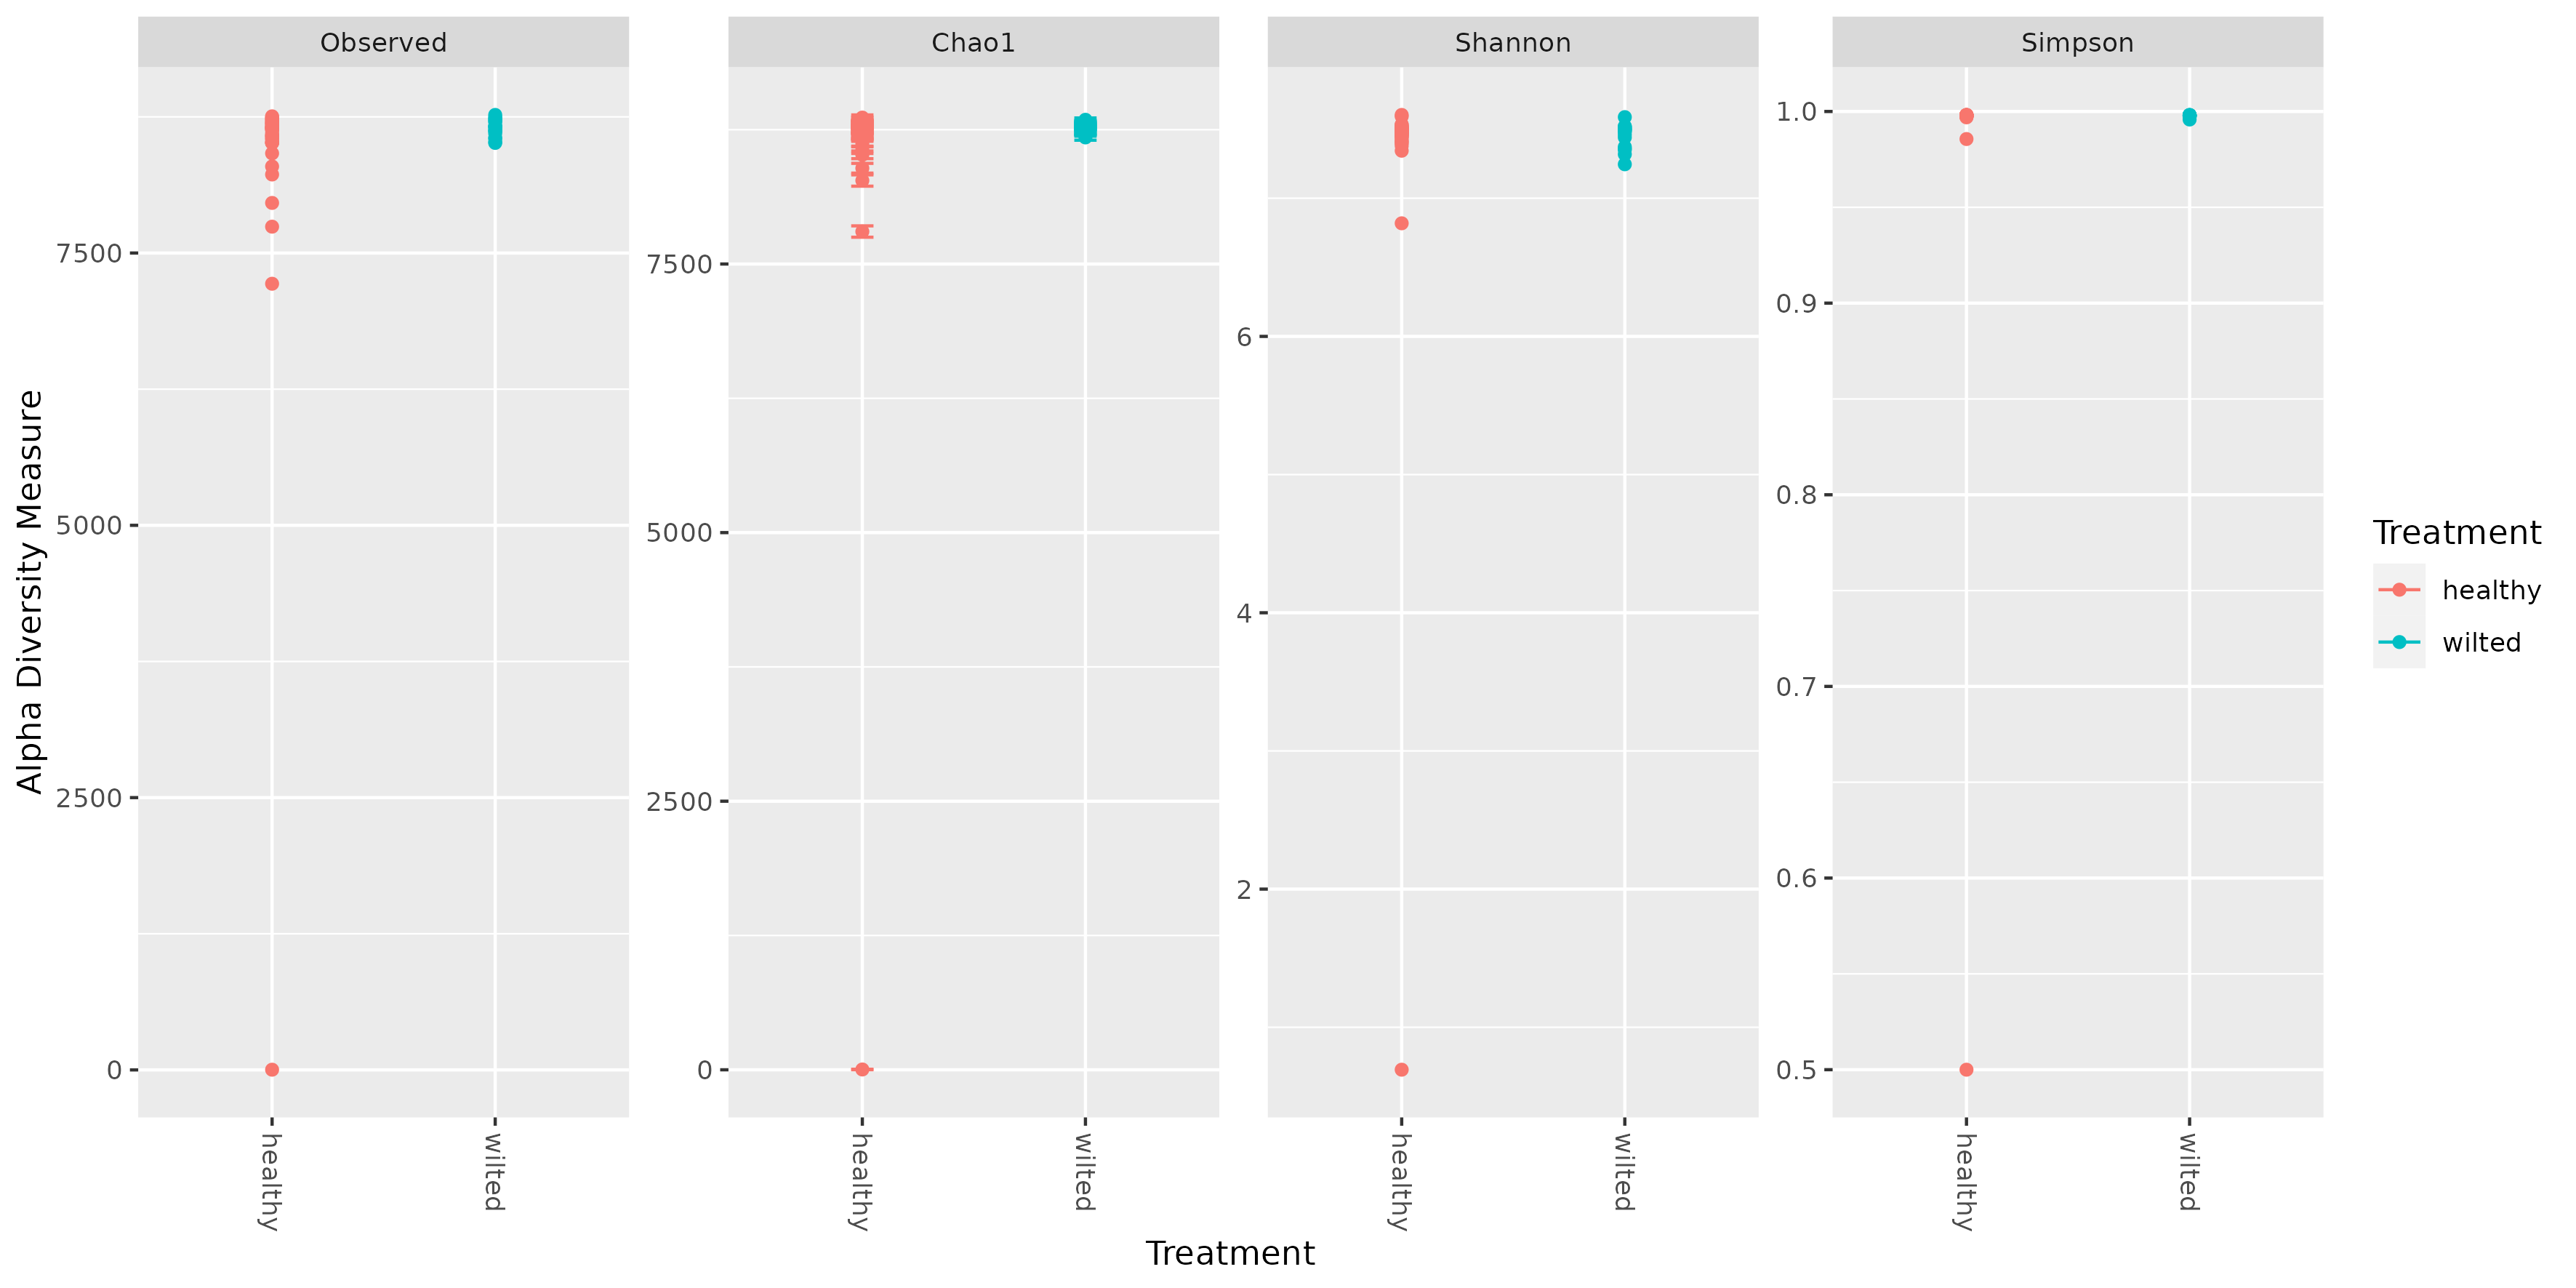
\includegraphics[width=\textwidth]{Img/cap2/DiversidadAlfaFresaKraken.png}
\caption{Diversidad alfa datos crudos metagenomicos de fresa, \href{https://github.com/CamilaSilva1995/Tesis_Maestria/blob/main/Analisis_Comparativo/Fresa_Solena/01_Exploracion.Rmd}{(Exploracion.Rmd)} }
\end{figure}

En la imagen, se pueden identificar datos no deseados que afectan la visualización, por lo que se lleva a cabo un filtro de calidad de los datos.\\

Eliminar muestras de baja calidad resulta en una mejora significativa en la claridad y la interpretación de la visualización. La diferencia es notable después de descartar las muestras de baja calidad, lo que resalta la importancia de un proceso riguroso de filtrado para obtener resultados más precisos y confiables. Este enfoque contribuye a una representación más fiel de los datos, permitiendo una interpretación más precisa y una toma de decisiones informada.\\

\begin{figure}[h]
\centering
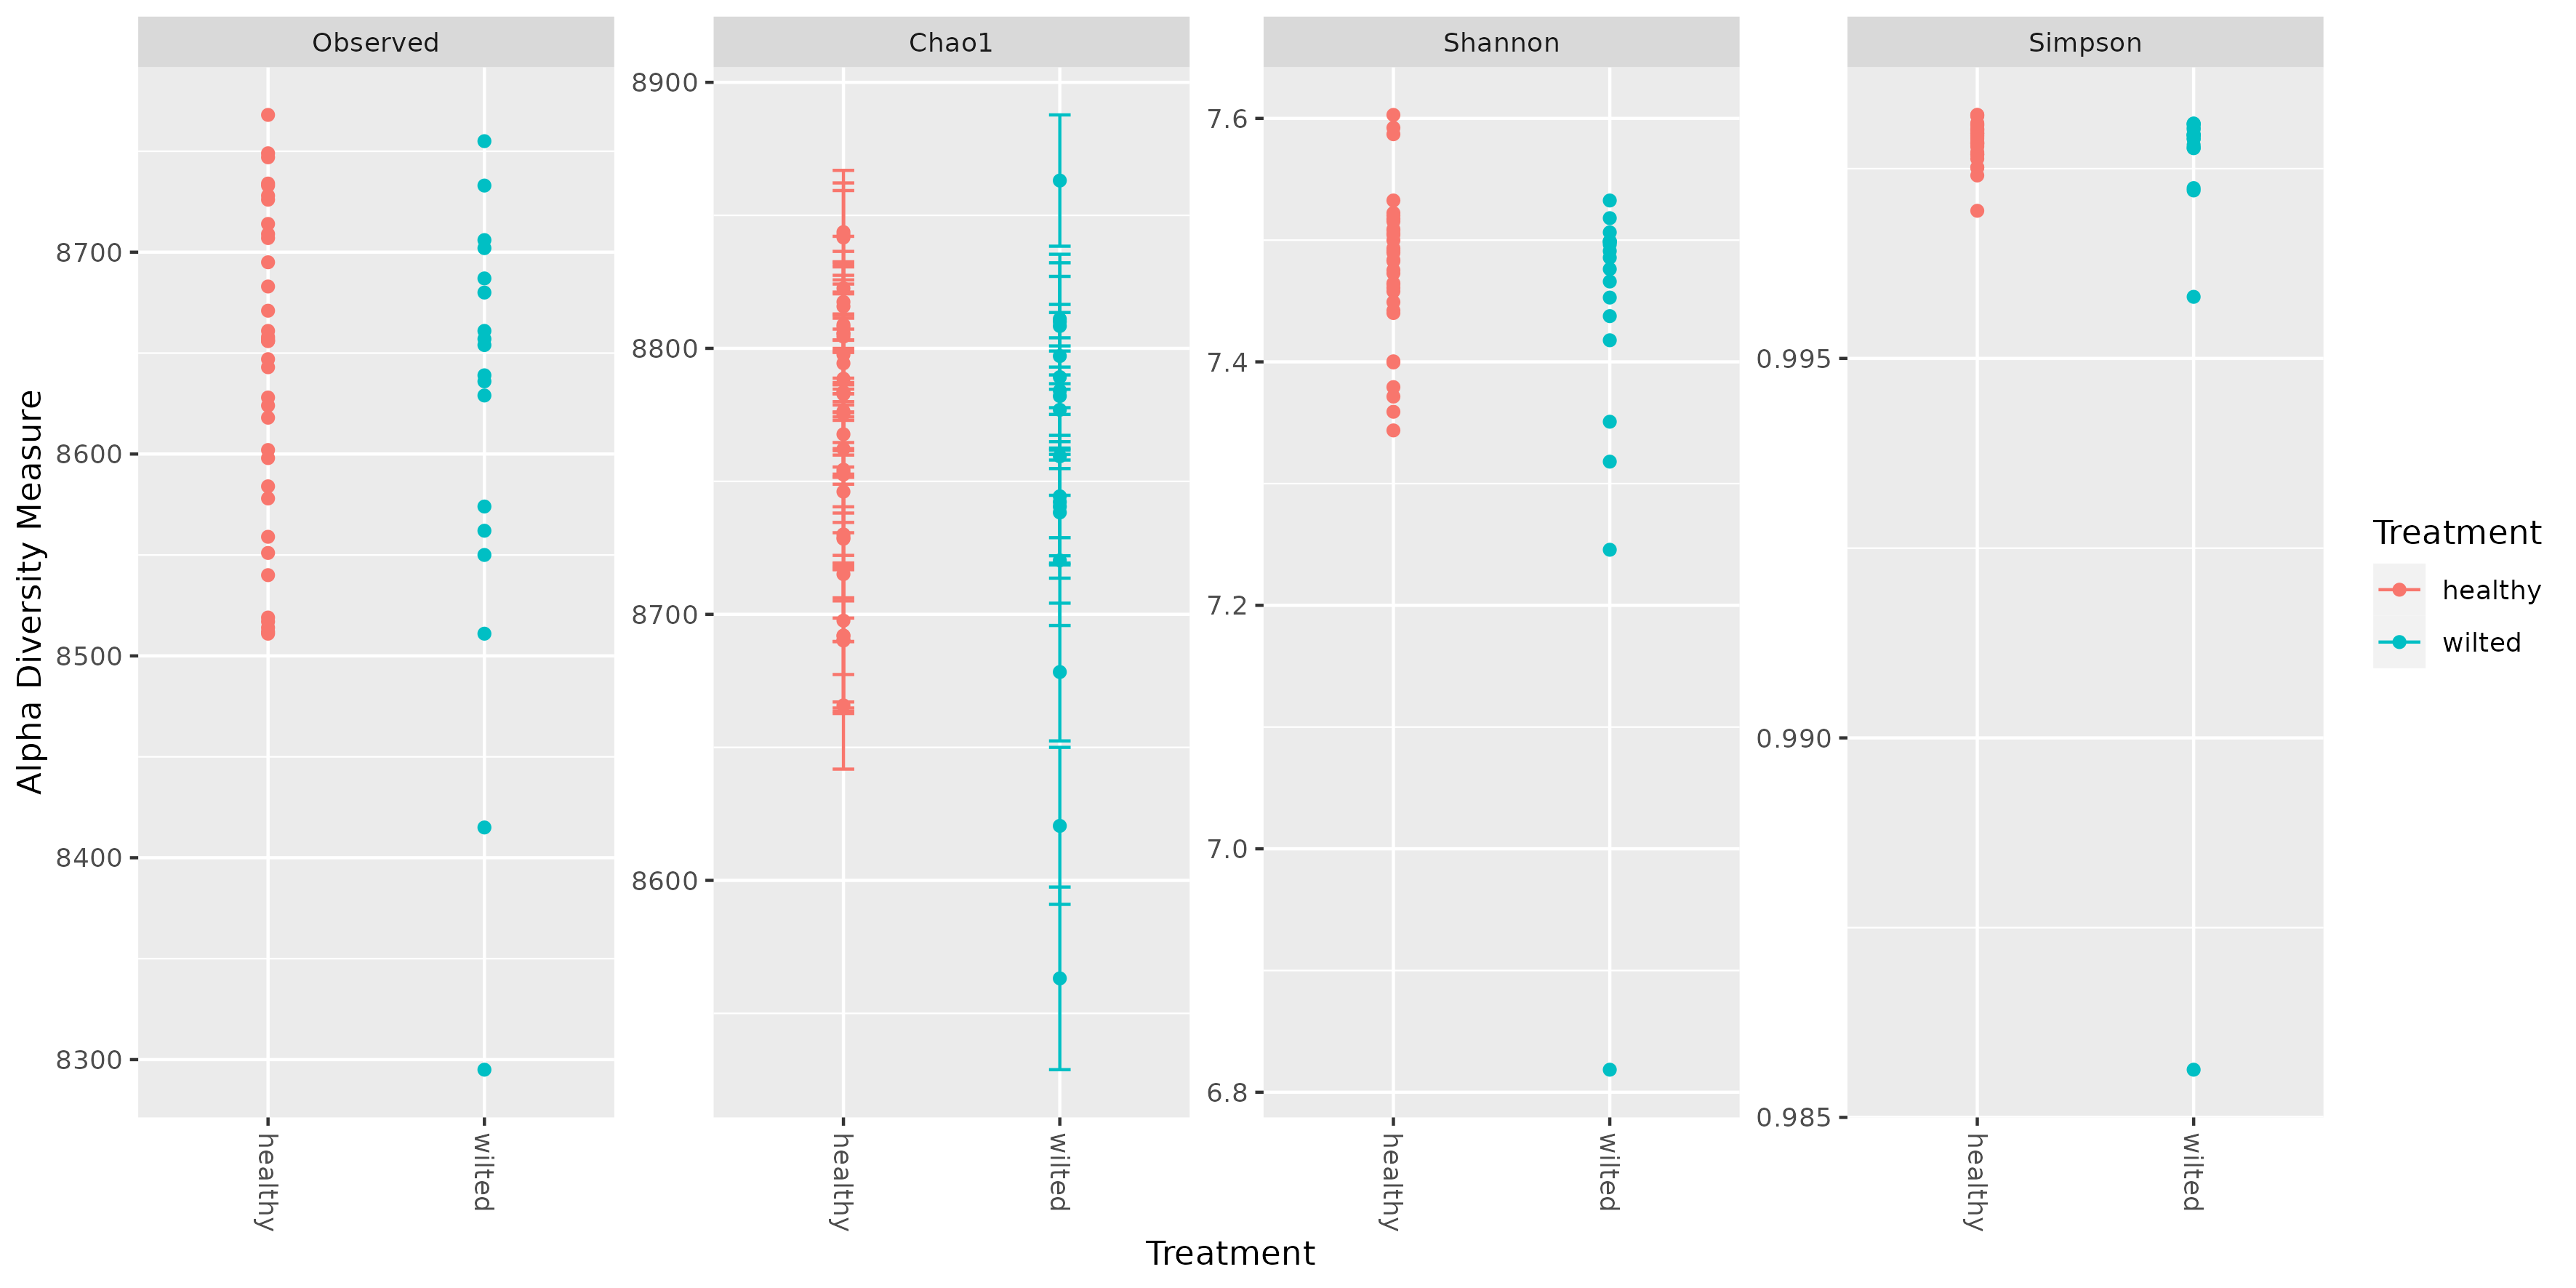
\includegraphics[width=\textwidth]{Img/cap2/DiversidadAlfaFresaKraken_fil.png}
\caption{Diversidad alfa datos filtrados metagenomicos de fresa, \href{https://github.com/CamilaSilva1995/Tesis_Maestria/blob/main/Analisis_Comparativo/Fresa_Solena/01_Exploracion.Rmd}{(Exploracion.Rmd)} }
\end{figure}

Después de aplicar el filtro de calidad de los datos, la visualización de la diversidad alfa en los conjuntos de muestras de plantas sanas y enfermas revela una mayor diversidad en las muestras sanas en comparación con las muestras enfermas. Esta observación se confirma mediante la métrica Chao1, que elimina la influencia de los singletons y doubletons, respaldando la percepción visual de una mayor diversidad en las muestras sanas. A pesar de la diferencia en las diversidades observadas, cabe destacar que esta disparidad no es significativamente grande, sugiriendo que no hay una diferencia sustancial en la diversidad entre las muestras sanas y enfermas.\\

Este análisis proporciona una evaluación más completa de la diversidad alfa, indicando que aunque hay variaciones discernibles, estas no son lo suficientemente notables como para afirmar una gran disparidad en la diversidad entre los conjuntos de muestras. Este tipo de conclusiones respaldadas por métricas específicas y visualizaciones contribuyen a una interpretación más precisa de la composición de las comunidades microbianas en plantas sanas y enfermas\\

\subsection{Diversidad Beta}
La diversidad beta se encarga de evaluar cuán similares o diferentes son un par de especies, muestras, conjuntos de muestras o poblaciones entre sí. Fue definida por Whittaker como una medida del cambio de diversidad a traves de gradientes ambientales, en otras palabras "tasa de cambio en la composisión de especies de una comunidad a otra a los largo de gradientes" (\cite{whittaker1960}). Para medir esta diversidad, se utilizan métricas como la disimilitud de Bray-Curtis, la distancia Jaccard o la distancia UniFrac.\\

Antes de realizar análisis de diversidad beta, es crucial convertir las abundancias absolutas (número de lecturas por OTU) a relativas (porcentajes de lecturas asignadas a un OTU dentro de una muestra). Esta transformación es esencial debido a que los metagenomas tienen tamaños diferentes. Se lleva a cabo el cálculo de las abundancias relativas utilizando la función 'transform\_sample' de Phyloseq, tanto para los datos originales como para los datos filtrados.\\

Este paso es fundamental para garantizar una comparación y evaluación adecuada de la diversidad beta, ya que las abundancias relativas proporcionan una representación más precisa de la estructura de la comunidad, independientemente de las diferencias en el tamaño del metagenoma entre las muestras.\\

\begin{lstlisting}[basicstyle=\small] 
transform_sample_counts(fresa_kraken_fil,
function(x) x*100/sum(x) )
\end{lstlisting}

Usamos “ordinate” para asignar las distancias entre muestras, iniciando y tomando como referencia “Bray-Curtis”, ya que es una de las
metricas mas completas y mayormente utilizadas para medir la diversidad beta.\\

Para visualizar y presentar los resultados de este análisis, se opta por el uso de NMDS (Non-metric Multidimensional Scaling), una herramienta de análisis exploratorio de datos que se emplea para visualizar la similitud o disimilitud entre una colección de objetos (por ejemplo, especies, sitios, genes) en un espacio de baja dimensionalidad. Entre otros, se utilizan ampliamente los análisis PCA, PCoA o NMDS.\\

A continuación, se presenta una lista de distancias disponibles que Phyloseq puede utilizar, siendo las siguientes las más comúnmente utilizadas:\\

La \textbf{Disimilitud de Bray-Curtis}es un índice que se fundamenta en la composición y abundancia de especies en diferentes sitios (\cite{bray&curtis1957}). Este índice mide la similitud entre dos muestras o poblaciones en términos de las especies que comparten, considerando la ponderación de la abundancia de cada especie en cada población.

La fórmula del índice de disimilitud de Bray-Curtis es:
$$d_{BC} = 1 - \frac{2S}{(S_{a} + S_{b})}$$
donde $d_{BC}$ es el índice de disimilitud de Bray-Curtis, $S$ es el número de especies compartidas entre las poblaciones $a$ y $b$, y $S_{a}$ y $S_{b}$ son los números de especies exclusivas de los sitios $a$ y $b$, respectivamente.\\

Este índice proporciona una medida cuantitativa de la diferencia relativa en términos de composición de especies y abundancia entre dos poblaciones o muestras. Cuanto más cercano a 1 sea el valor del índice, mayor será la disimilitud entre las poblaciones.\\

\begin{figure}[h]
\centering
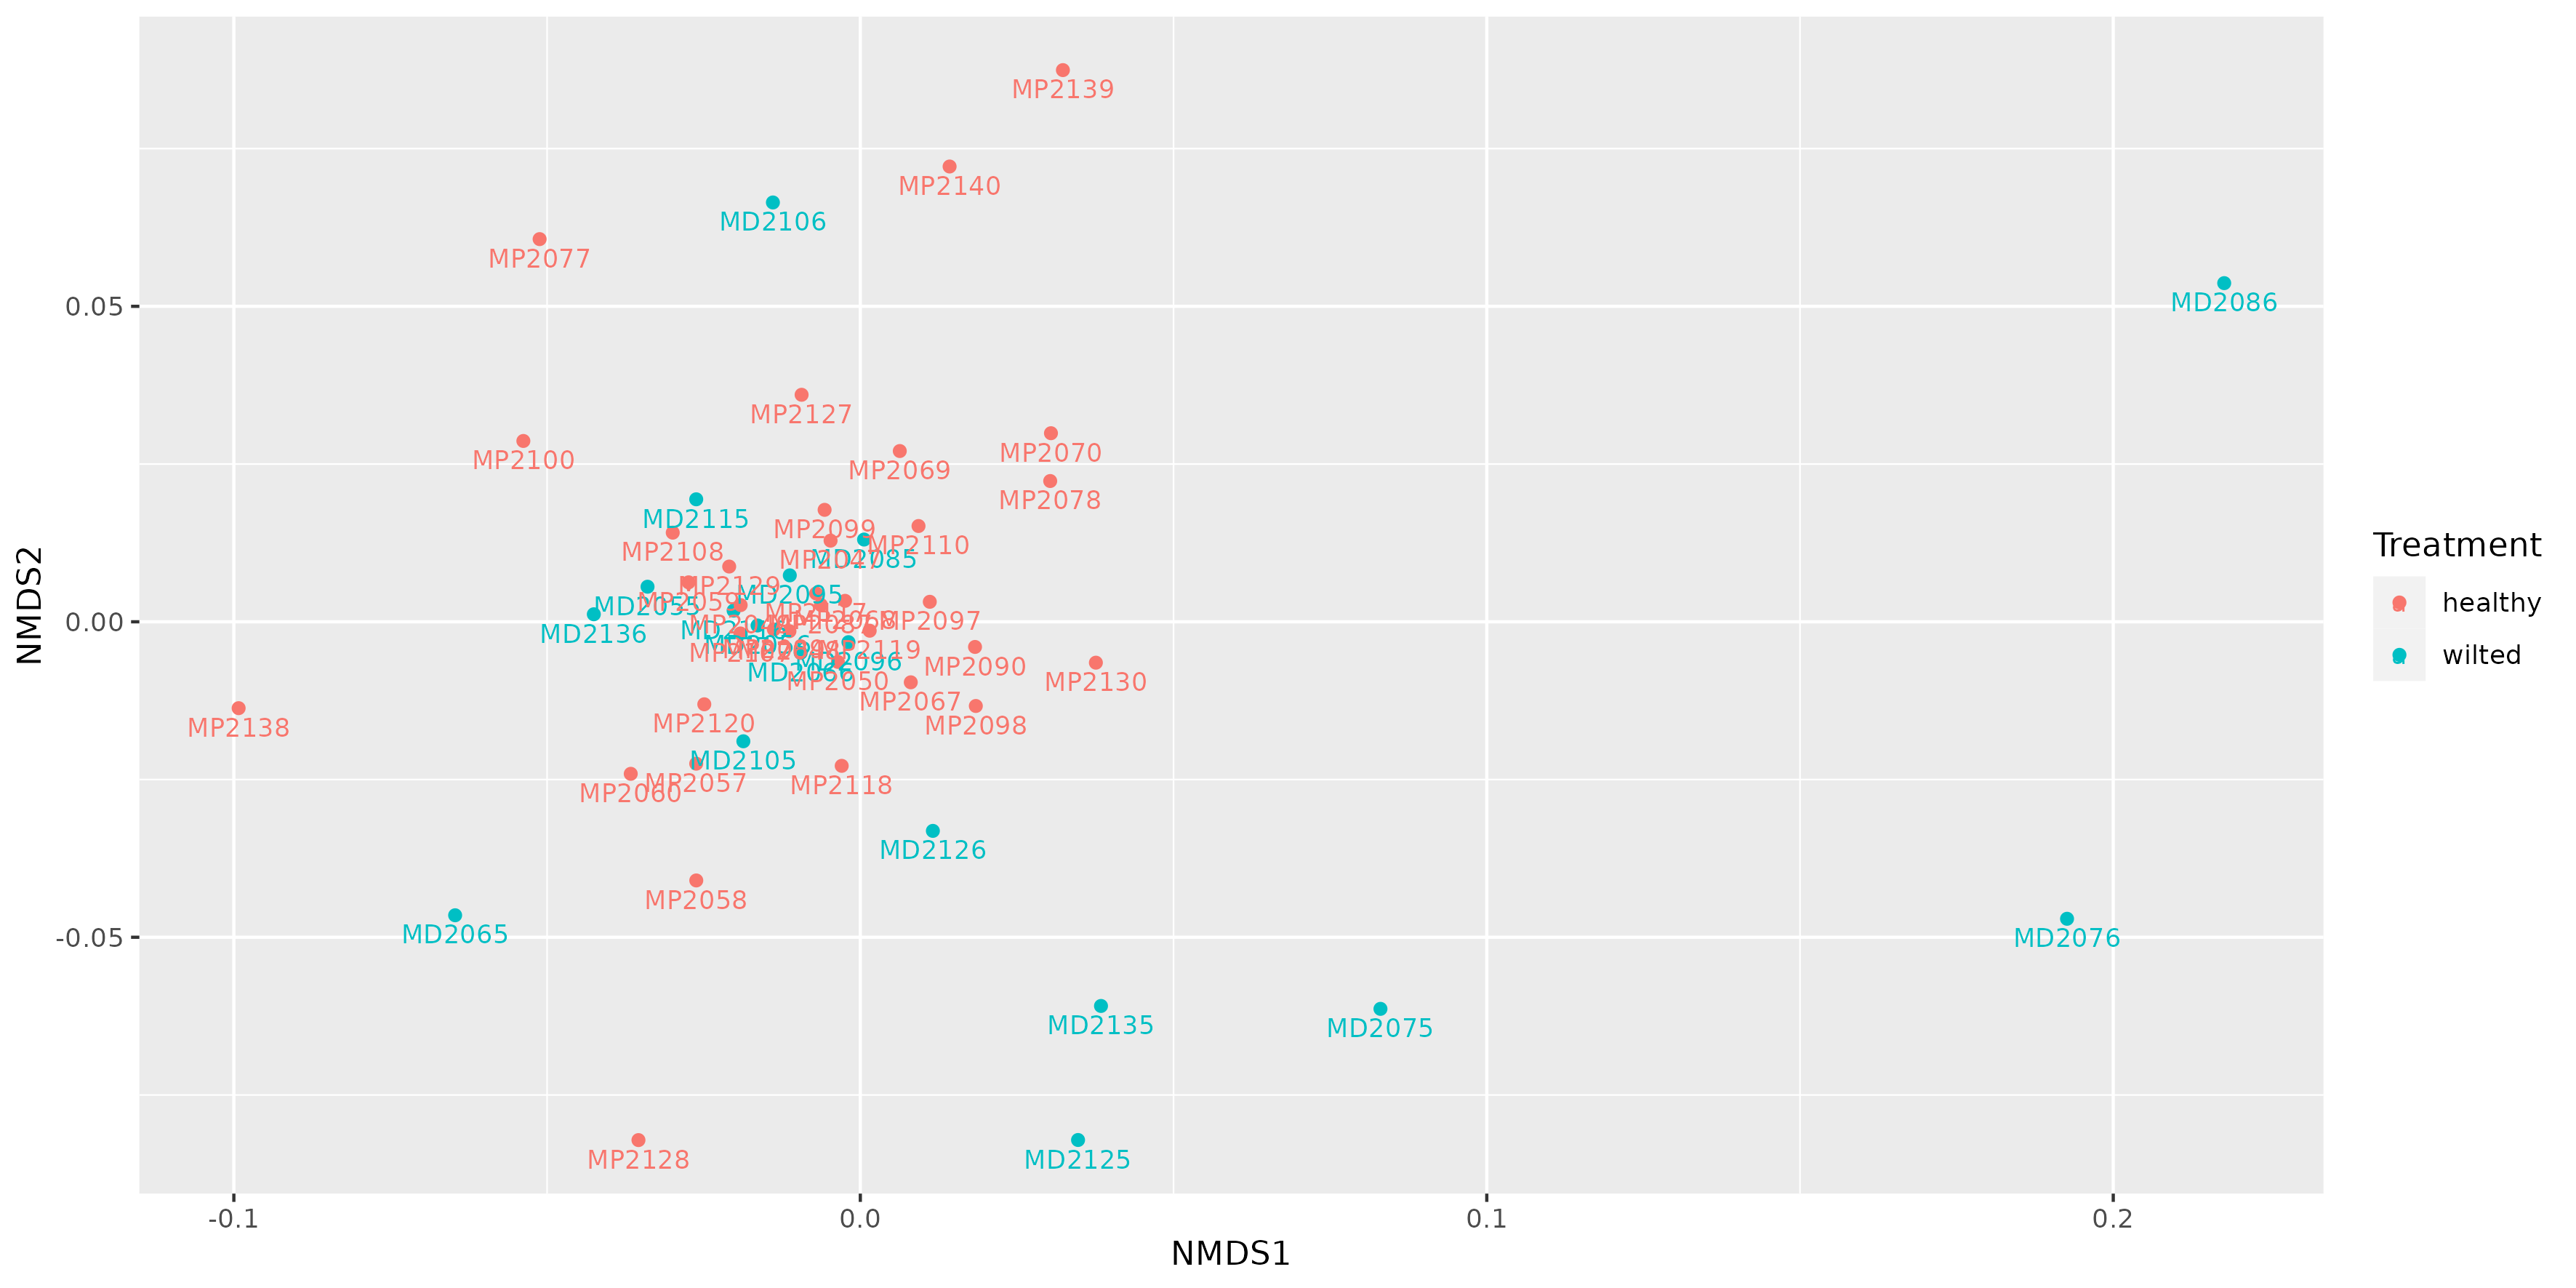
\includegraphics[width=\textwidth]{Img/cap2/DiversidadBetaFresaKraken_fil.png}
\caption{Diversidad Beta, disimilitud de Bray-Curtis,  \href{https://github.com/CamilaSilva1995/Tesis_Maestria/blob/main/Analisis_Comparativo/Fresa_Solena/01_Exploracion.Rmd}{(Exploracion.Rmd)}}
\end{figure}

La \textbf{Distancia Jaccard} es un índice de disimilitud que se basa en la presencia o ausencia de especies en diferentes poblaciones. Este índice compara la proporción de especies que son comunes entre dos poblaciones en relación con el total de especies encontradas en ambas poblaciones. Resulta útil para comparar la diversidad de especies entre diferentes poblaciones o evaluar la similitud en la composición de especies entre comunidades diversas.

La fórmula para el índice de disimilitud de Jaccard es la siguiente:
$$d_{JC} = 1 - \frac{S}{(S_{a} + S_{b}-S)}$$
donde $d_{JC}$ es el índice de disimilitud de Jaccard, $S$ es el número de especies compartidas entre las poblaciones $a$ y $b$, y $S_{a}$ y $S_{b}$ son los números de especies exclusivas de los sitios $a$ y $b$, respectivamente.\\

Este índice ofrece una medida de disimilitud que se centra en la presencia o ausencia de especies, siendo 0 cuando las poblaciones comparten todas las especies y 1 cuando no comparten ninguna. Es especialmente útil para análisis comparativos de la composición de especies entre diferentes comunidades.\\

\begin{figure}[!]
\centering
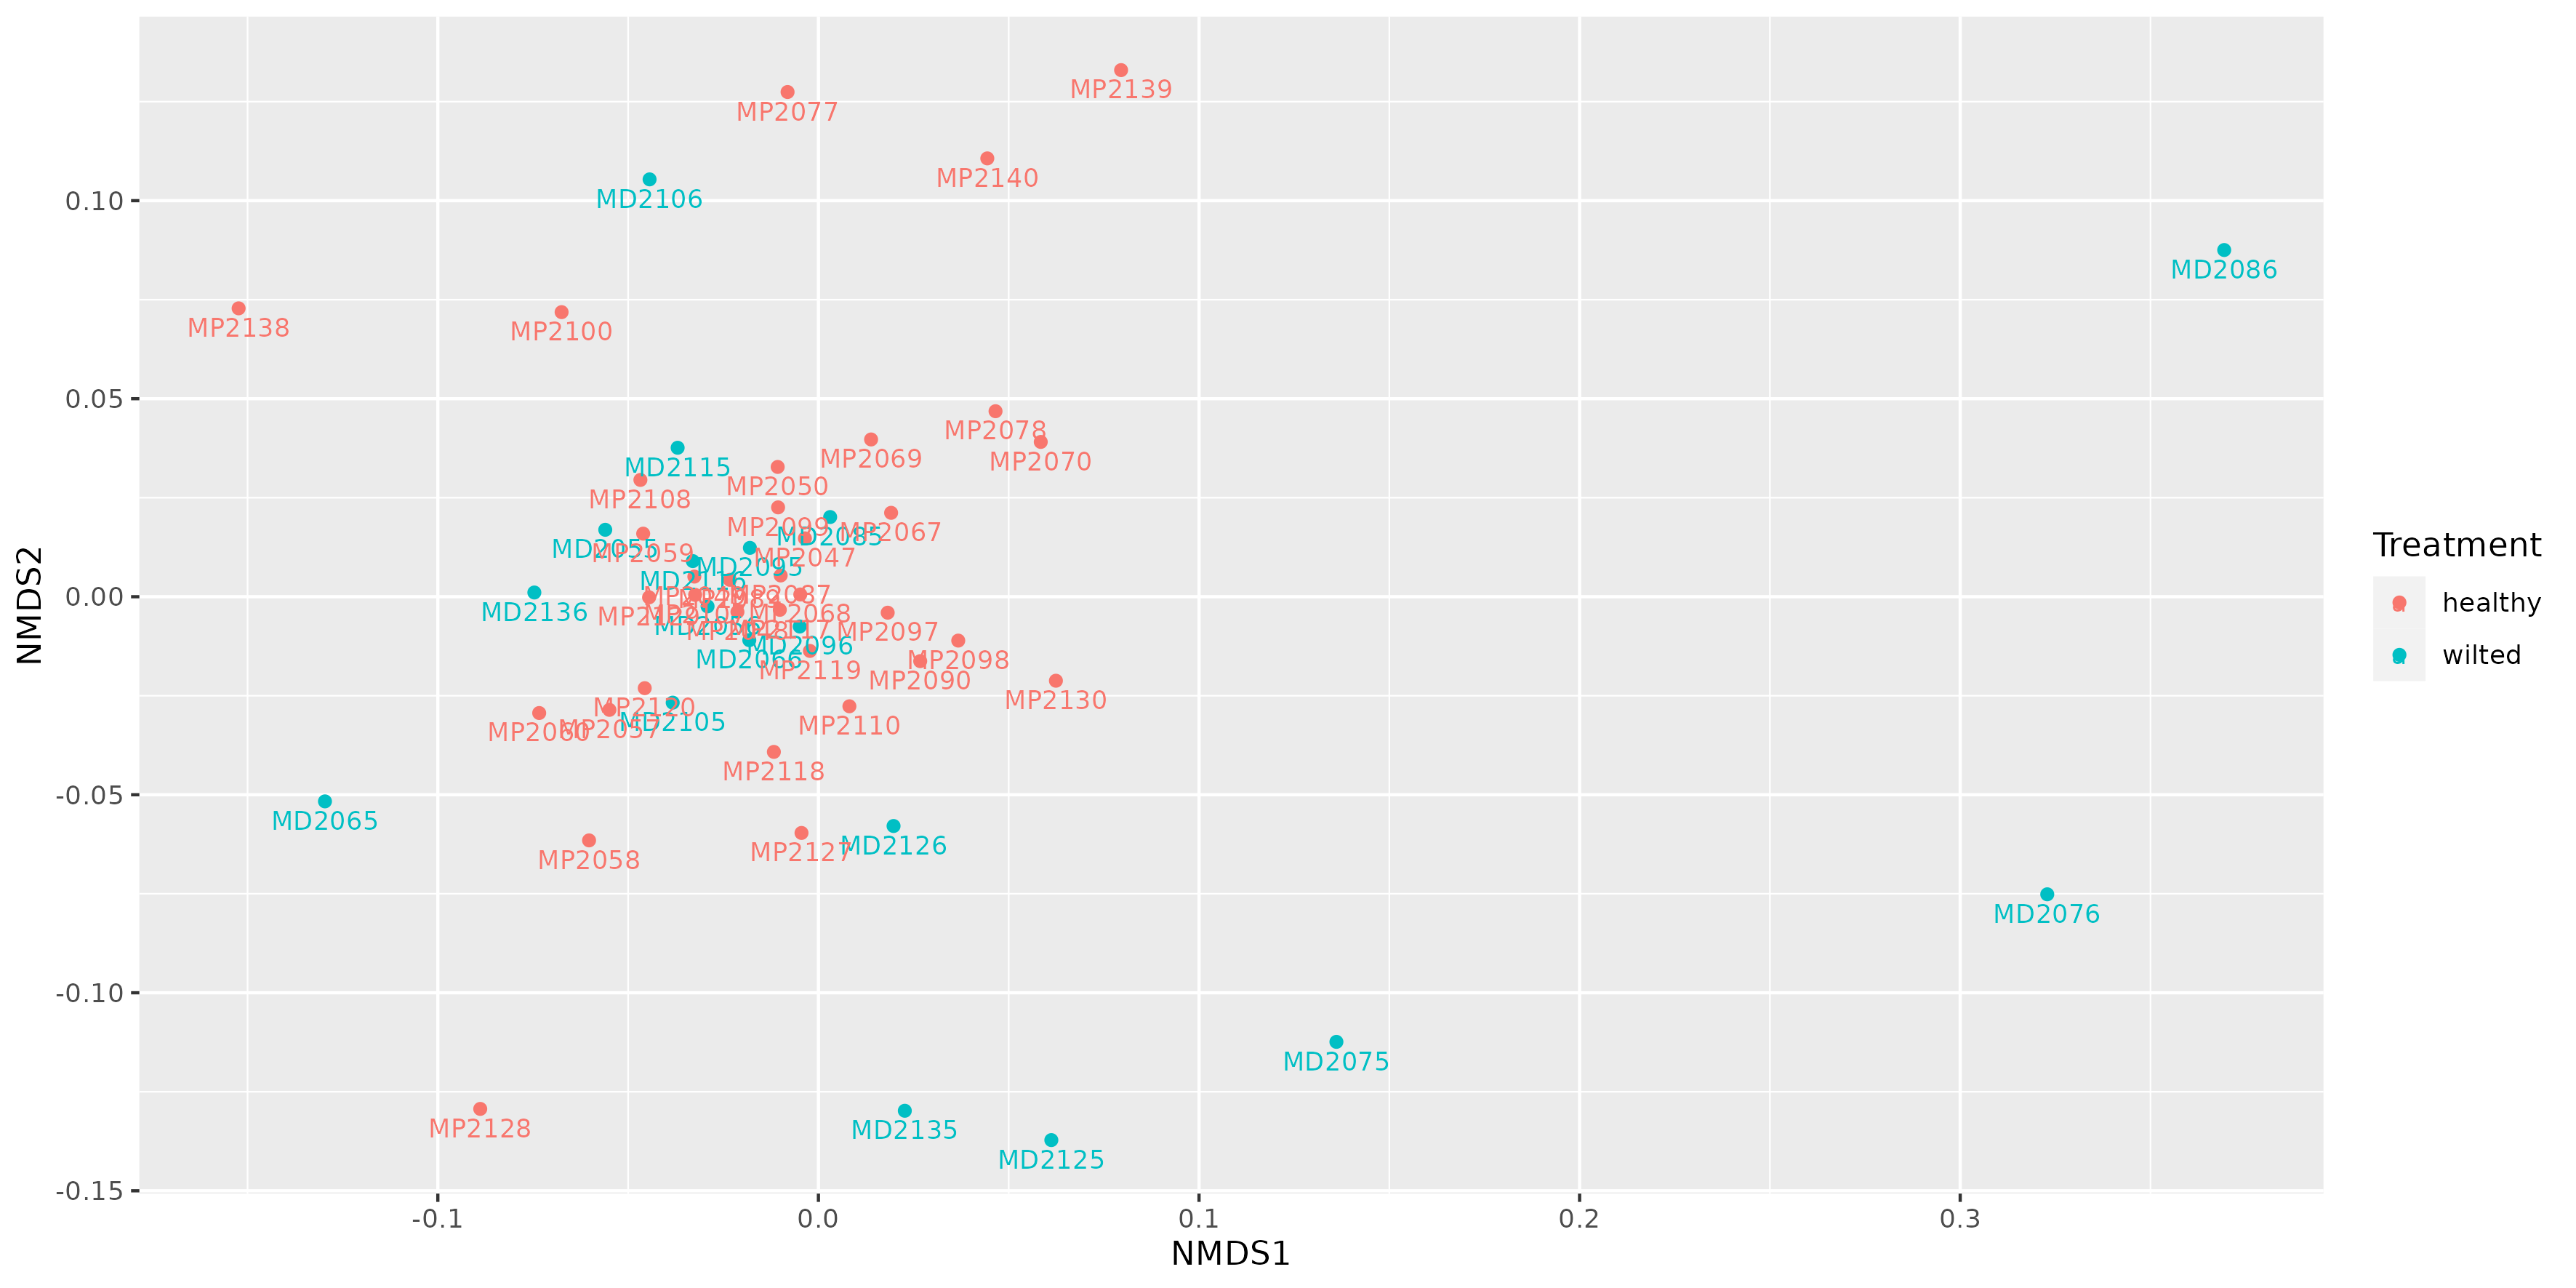
\includegraphics[width=\textwidth]{Img/cap2/DiversidadBetaFresaKraken_fil_jaccard.png}
\caption{Diversidad Beta, distancia de Jaccard, \href{https://github.com/CamilaSilva1995/Tesis_Maestria/blob/main/Analisis_Comparativo/Fresa_Solena/01_Exploracion.Rmd}{(Exploracion.Rmd)}}
\end{figure}

Tomando los datos con filtro de calidad y utilizando la distancia de Jaccard, la cual es la más comúnmente utilizada en este tipo de estudios, se observa que las muestras, tanto sanas como enfermas, están bastante mezcladas. Ante esta observación, se procede a realizar pruebas con distintas distancias para explorar si alguna otra métrica puede proporcionar una separación más clara o revelar patrones específicos en la composición de especies entre las muestras.\\

La distancia \textbf{Euclideana}es comúnmente utilizada en el análisis de datos numéricos y se fundamenta en la diferencia de las abundancias o proporciones de diferentes especies en distintas muestras. Esta distancia mide la separación entre dos muestras como la raíz cuadrada de la suma de las diferencias cuadráticas entre las proporciones de cada especie en ambas muestras.

La fórmula para la distancia Euclidiana entre dos muestras $A$ y $B$ es la siguiente:
$$d_{euclidean} (A,B) = \sqrt{\sum(A_i - B_i)^2}$$
Donde $A_i$ y $B_i$ son las abundancias o proporciones de la especie $i$ en las muestras $A$ y $B$, respectivamente.\\

La distancia Euclidiana es simétrica y cumple con la desigualdad del triángulo, lo que significa que satisface las propiedades de una verdadera distancia. Esta métrica es especialmente adecuada para comparar muestras en términos de diferencias numéricas en las abundancias de las especies.\\

\begin{figure}[!]
\centering
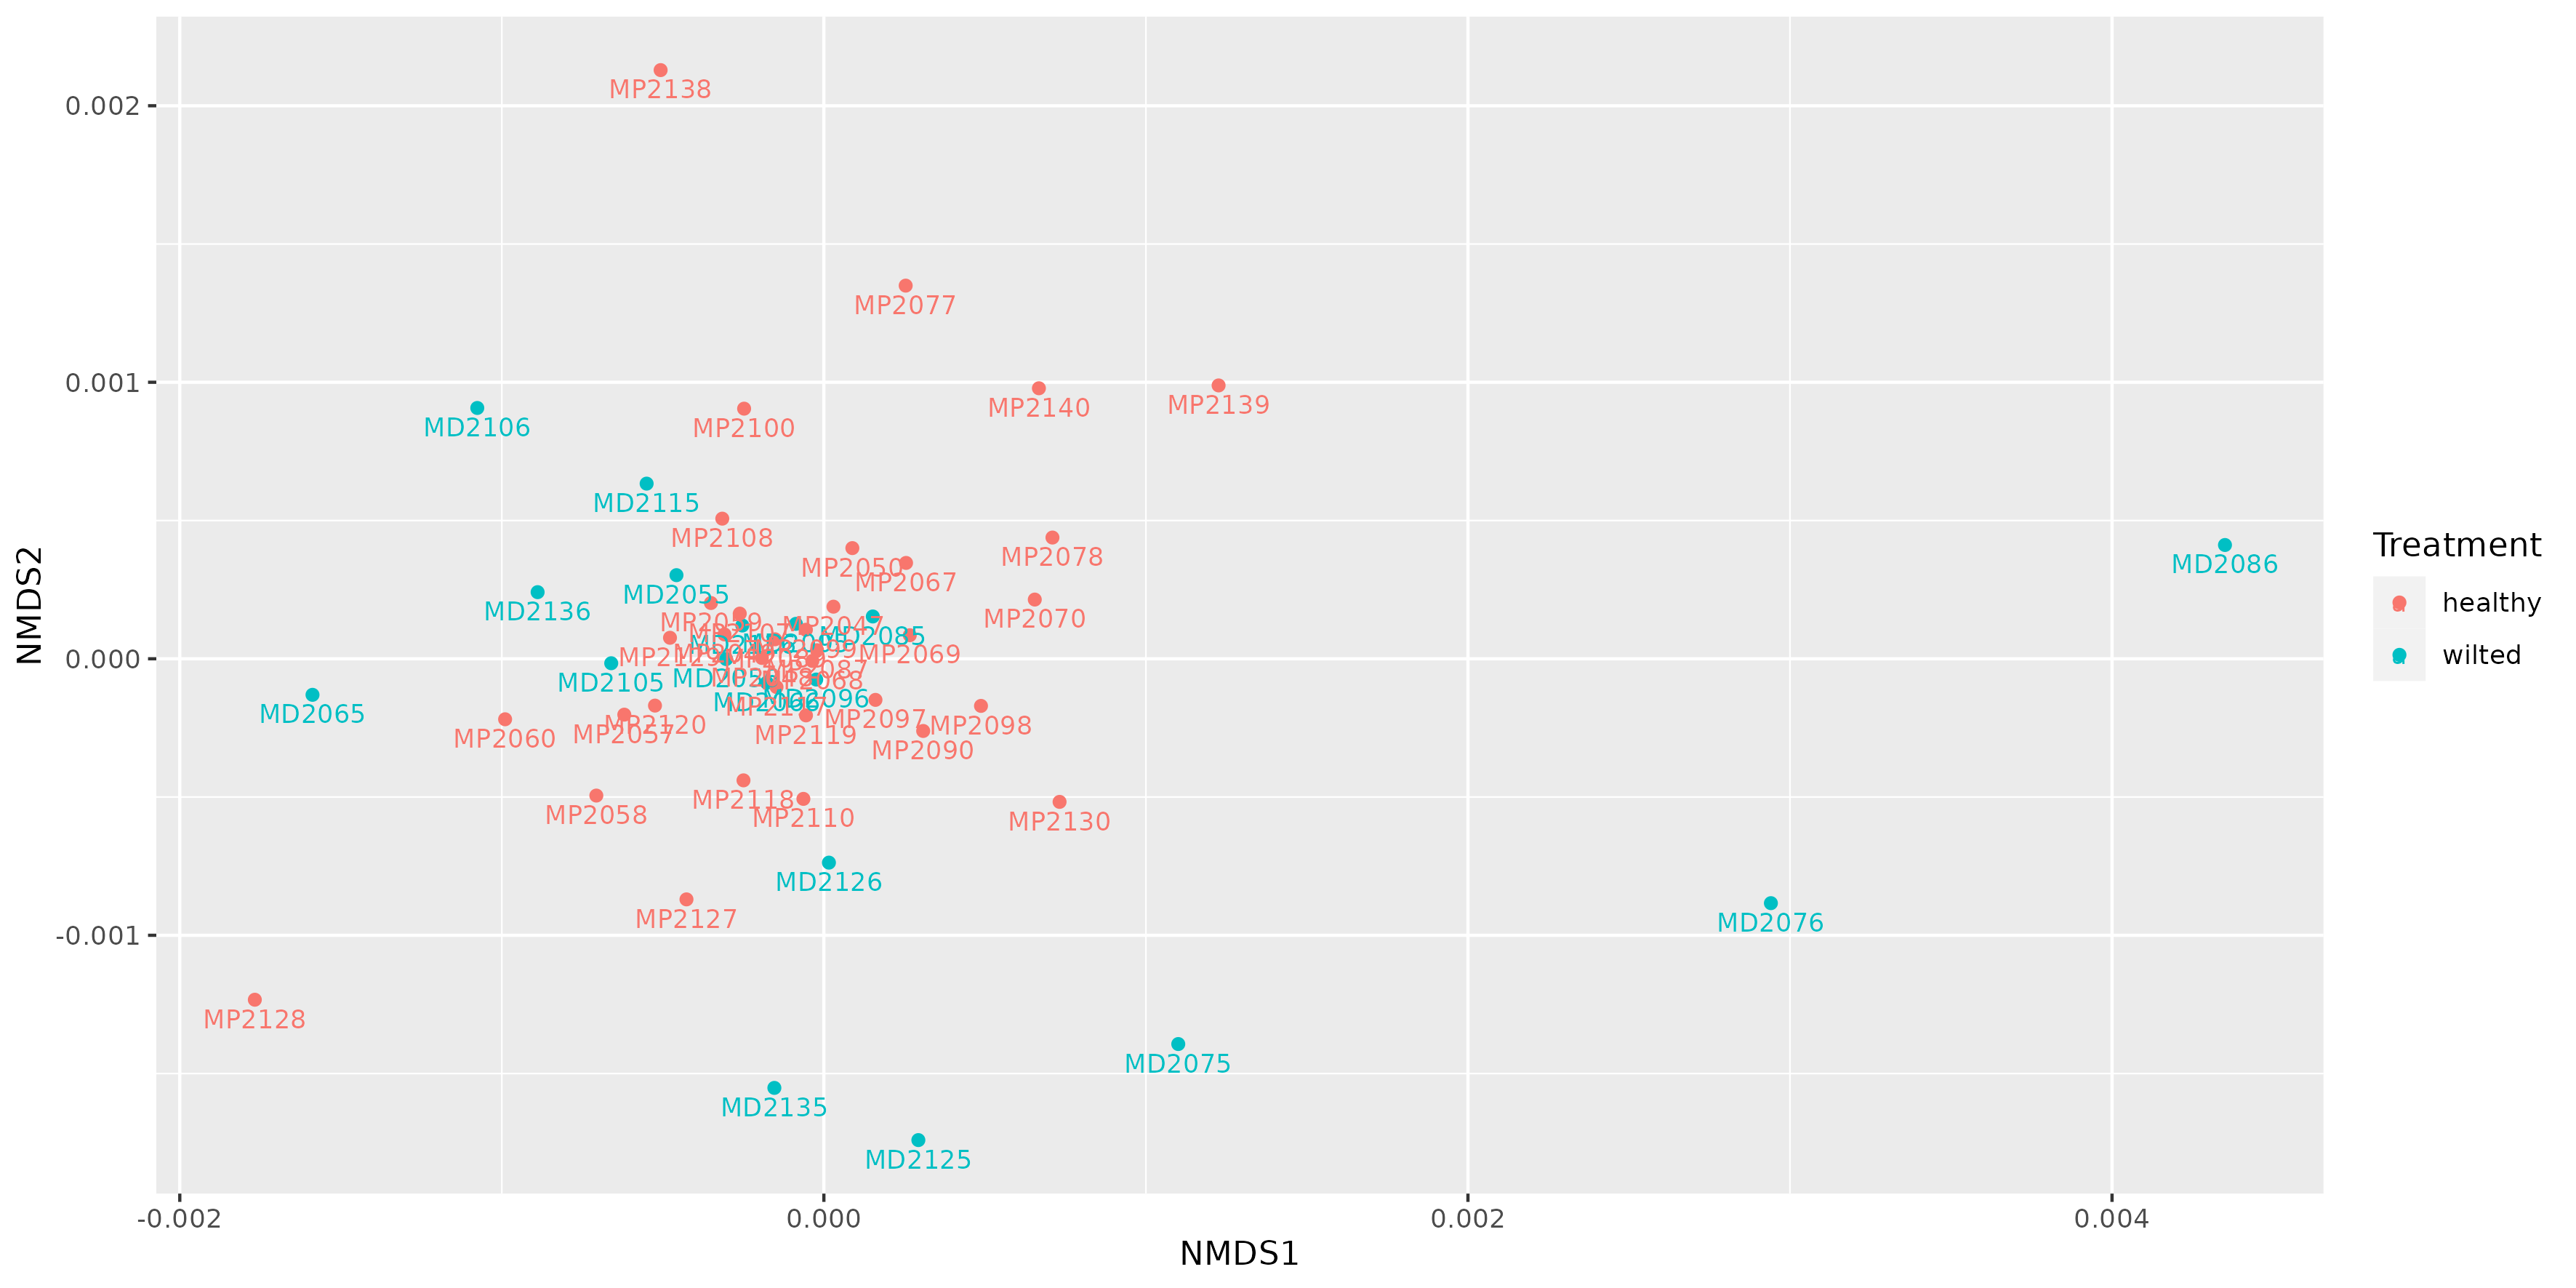
\includegraphics[width=\textwidth]{Img/cap2/DiversidadBetaFresaKraken_fil_euclidean.png}
\caption{Diversidad Beta, distancia Euclidiana, \href{https://github.com/CamilaSilva1995/Tesis_Maestria/blob/main/Analisis_Comparativo/Fresa_Solena/01_Exploracion.Rmd}{(Exploracion.Rmd)}}
\end{figure}

La distancia \textbf{Manhattan} también se emplea en el análisis de datos numéricos y se basa en la diferencia de las abundancias o proporciones de diferentes especies en distintas muestras. En este caso, la distancia de Manhattan entre dos muestras se define como la suma de las diferencias absolutas entre las proporciones de cada especie en ambas muestras.

La fórmula de la distancia de Manhattan entre dos muestras $A$ y $B$ se calcula como:
$$d_{Manhattan}(A, B) = \sum{|A_i - B_i|}$$
Donde $A_i$ y $B_i$ son las abundancias o proporciones de la especie $i$ en las muestras $A$ y $B$, respectivamente. \\

Al igual que la distancia Euclidiana, la distancia de Manhattan es simétrica y satisface la desigualdad del triángulo. Esta métrica es adecuada para comparar muestras en términos de las diferencias absolutas en las abundancias de las especies.\\

\begin{figure}[!]
\centering
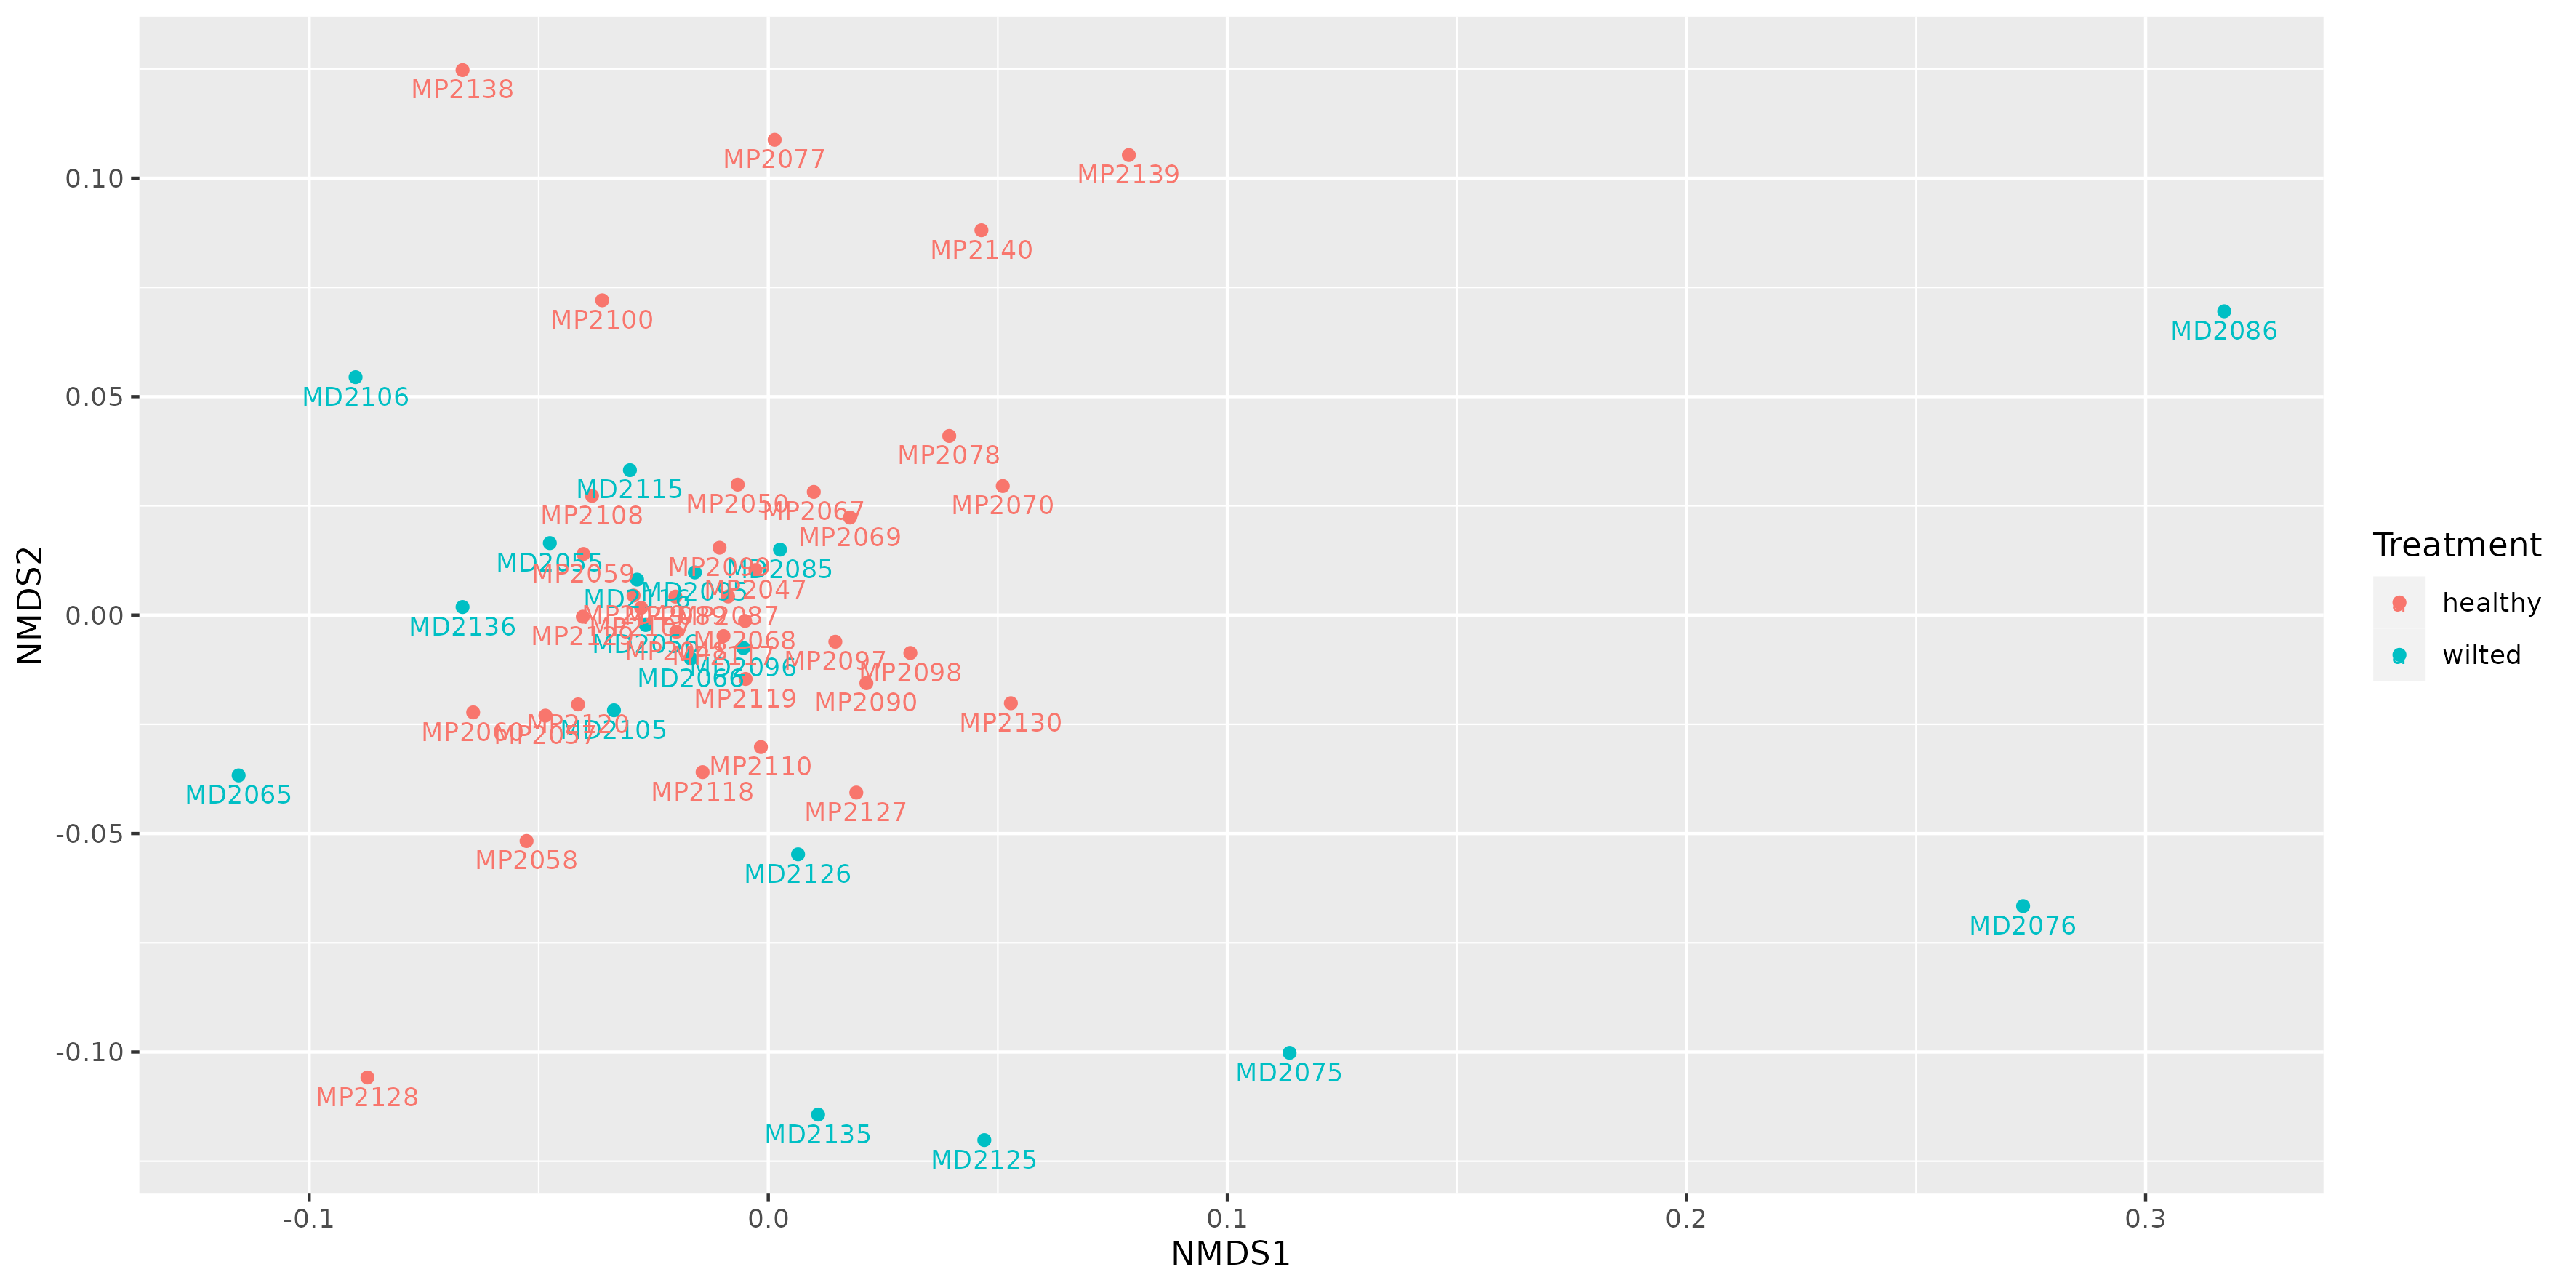
\includegraphics[width=\textwidth]{Img/cap2/DiversidadBetaFresaKraken_fil_manhattan.png}
\caption{Diversidad Beta, distancia Manhattan,  \href{https://github.com/CamilaSilva1995/Tesis_Maestria/blob/main/Analisis_Comparativo/Fresa_Solena/01_Exploracion.Rmd}{(Exploracion.Rmd)}}
\end{figure}

La \textbf{Divergencia de Jensen-Shannon (JSD)} se utiliza para comparar la similitud entre dos distribuciones de probabilidad. En el contexto del análisis de datos de diversidad, estas distribuciones de probabilidad pueden representar la proporción de diferentes especies en distintas muestras. La distancia de JSD entre dos distribuciones de probabilidad se calcula como la raíz cuadrada de la divergencia de Kullback-Leibler entre las dos distribuciones, dividida por dos. 

La fórmula de la distancia de JSD entre dos distribuciones de probabilidad $P$ y $Q$ es la siguiente:
$$d_{JSD}(P, Q) = \frac{\sqrt{(D_{KL}(P, M) + D_{KL}(Q, M))}}{2}$$
Donde $D_{KL}(P, M)$ y $D_{KL}(Q, M)$ son las divergencias de Kullback-Leibler entre las distribuciones $P$ y $Q$ y la media $M$ de ambas distribuciones, respectivamente. \\

Al igual que las distancias anteriores, la distancia de JSD es simétrica y satisface la desigualdad del triángulo. Esta métrica es especialmente útil cuando se quiere evaluar la similitud entre las proporciones de especies en diferentes muestras.\\

\begin{figure}[!]
\centering
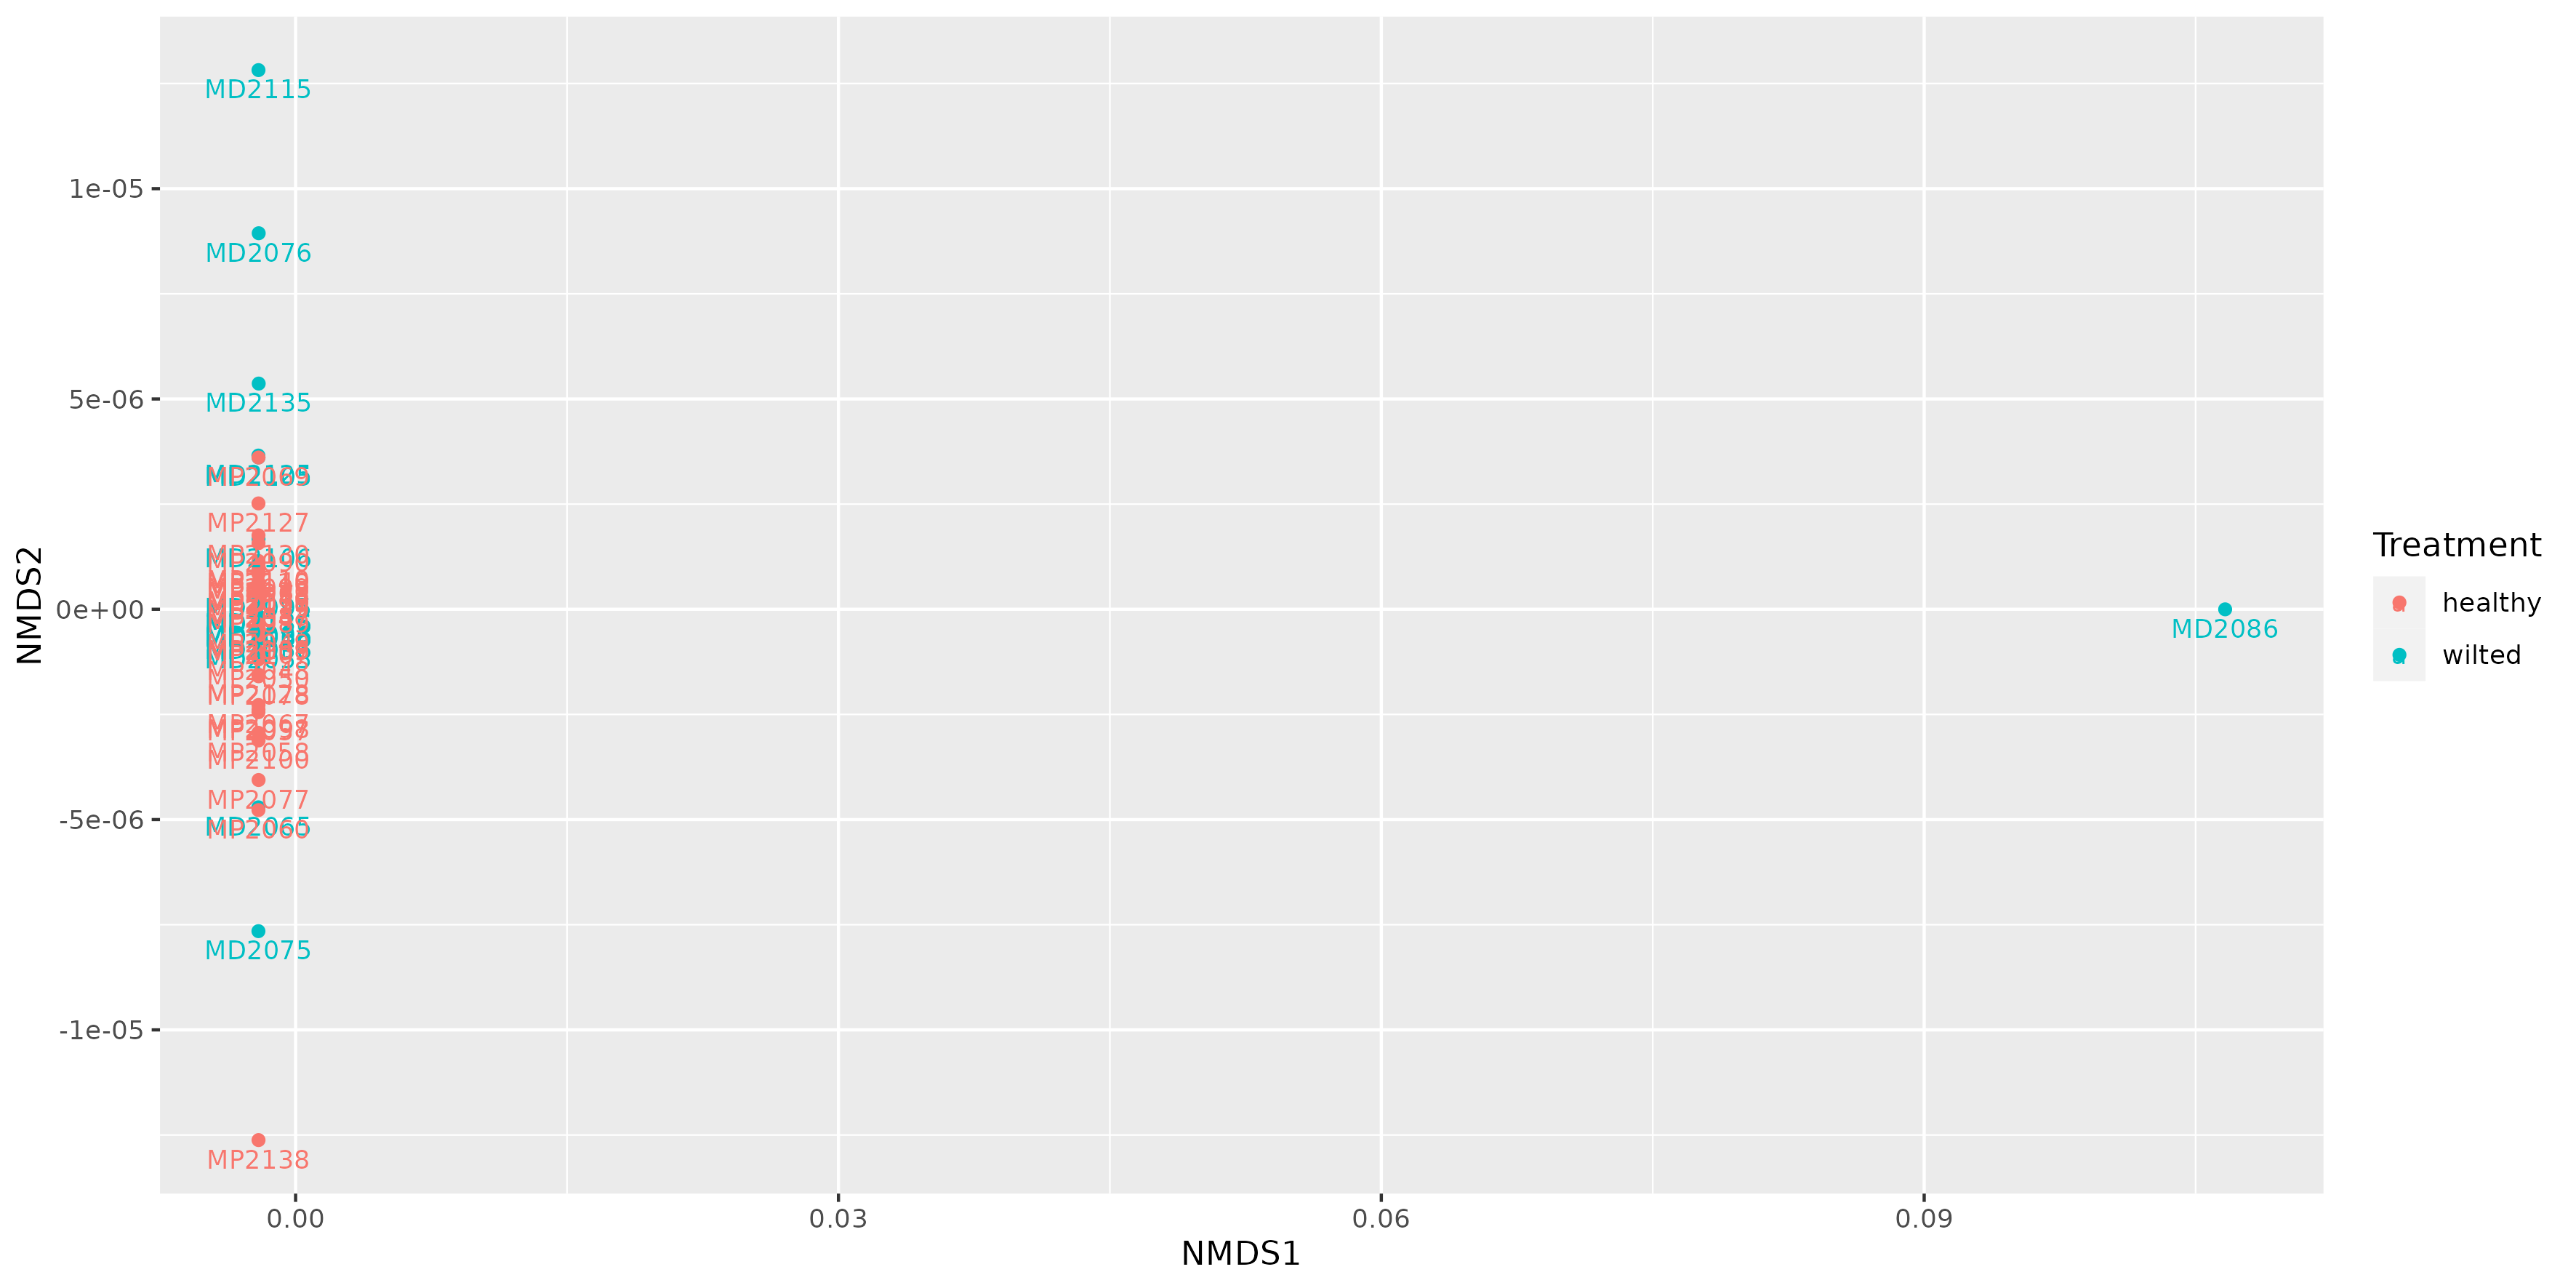
\includegraphics[width=\textwidth]{Img/cap2/DiversidadBetaFresaKraken_fil_jsd.png}
\caption{Diversidad Beta, divergencia de Jensen-Shannon,  \href{https://github.com/CamilaSilva1995/Tesis_Maestria/blob/main/Analisis_Comparativo/Fresa_Solena/01_Exploracion.Rmd}{(Exploracion.Rmd)}}
\end{figure}

La metrica de \textbf{UniFrac} es un índice de disimilitud que se basa en la filogenia de las especies presentes en diferentes sitios. Su objetivo es comparar la similitud entre dos sitios en términos de la diversidad filogenética de las especies, teniendo en cuenta la contribución relativa de cada rama en el árbol filogenético. Esta métrica resulta valiosa para evaluar la similitud en la evolución de las especies en diferentes comunidades o para comparar la estructura filogenética de distintas comunidades.\\

La fórmula del índice de disimilitud de UniFrac es más compleja en comparación con las de Bray-Curtis y Jaccard, ya que se basa en un análisis de la distribución de ramas filogenéticas únicas o compartidas entre los sitios. Este enfoque permite capturar la información sobre las relaciones evolutivas entre las especies, proporcionando una medida más completa de la similitud o disimilitud entre las comunidades estudiadas. \\

Estas métricas ofrecen diferentes perspectivas sobre la similitud o disimilitud entre muestras, permitiendo seleccionar la más apropiada según el contexto del estudio y los objetivos específicos del análisis de diversidad beta.\\

Luego de no ver una clara separacion de los datos, Dado que no se observa una clara separación de los datos, se decide proceder con un análisis en conjuntos más pequeños. Este enfoque puede ayudar a identificar patrones más específicos o diferencias significativas en la composición de especies entre subconjuntos de muestras, lo que contribuirá a una comprensión más detallada de la diversidad microbiana en el contexto particular del estudio.\\

\section{Exploración a distintos niveles taxonómicos}
Podemos visualizar las barras de abundancia absolutas y relativas de nuestros datos representando las muestras en el eje x y las abundancias en el eje y, diferenciando entre muestras sanas y enfermas.\\
\begin{figure}[h]
\centering
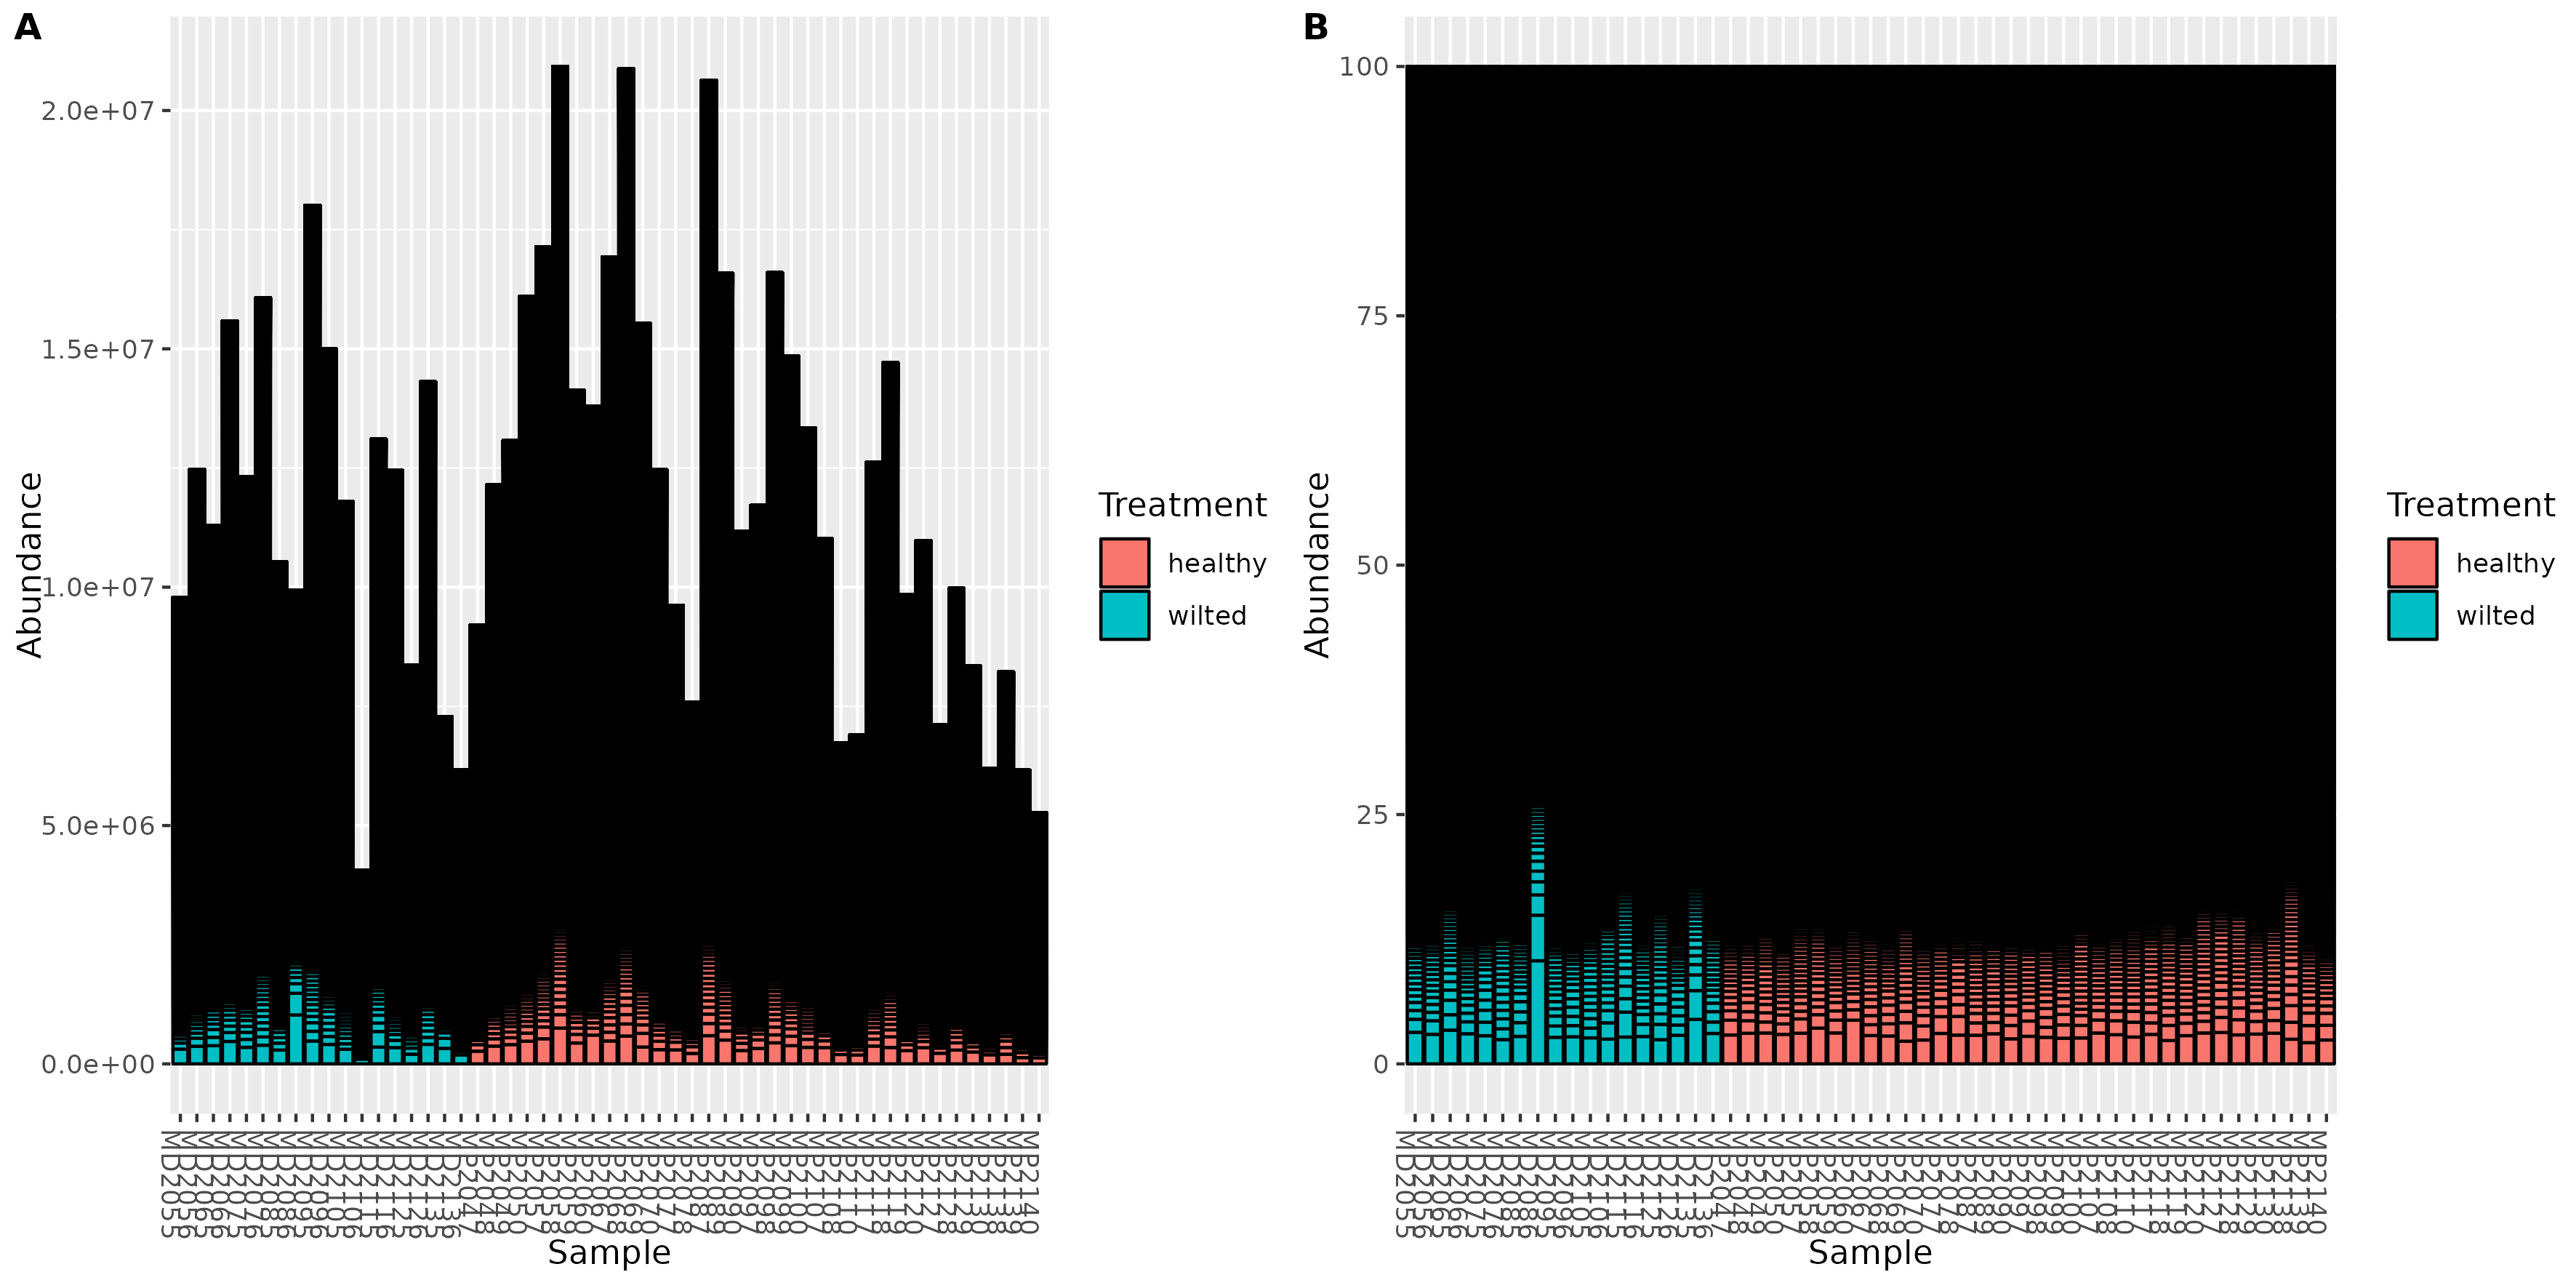
\includegraphics[width=\textwidth]{Img/cap2/Barras.png}
\caption{A) Barras de abundancias absolutas y B) Relativas}
\end{figure}
Debido a la gran cantidad de datos, resulta difícil discernir diferencias entre las muestras. Por lo tanto, se han creado subconjuntos dividiendo por reino y estableciendo subdivisiones en diferentes niveles taxonómicos.\\

A nivel de filo, ya podemos apreciar una mayor diversidad en nuestras muestras, siendo la mayoría de los filos pertenecientes a bacterias.\\
\begin{figure}[h]
\centering
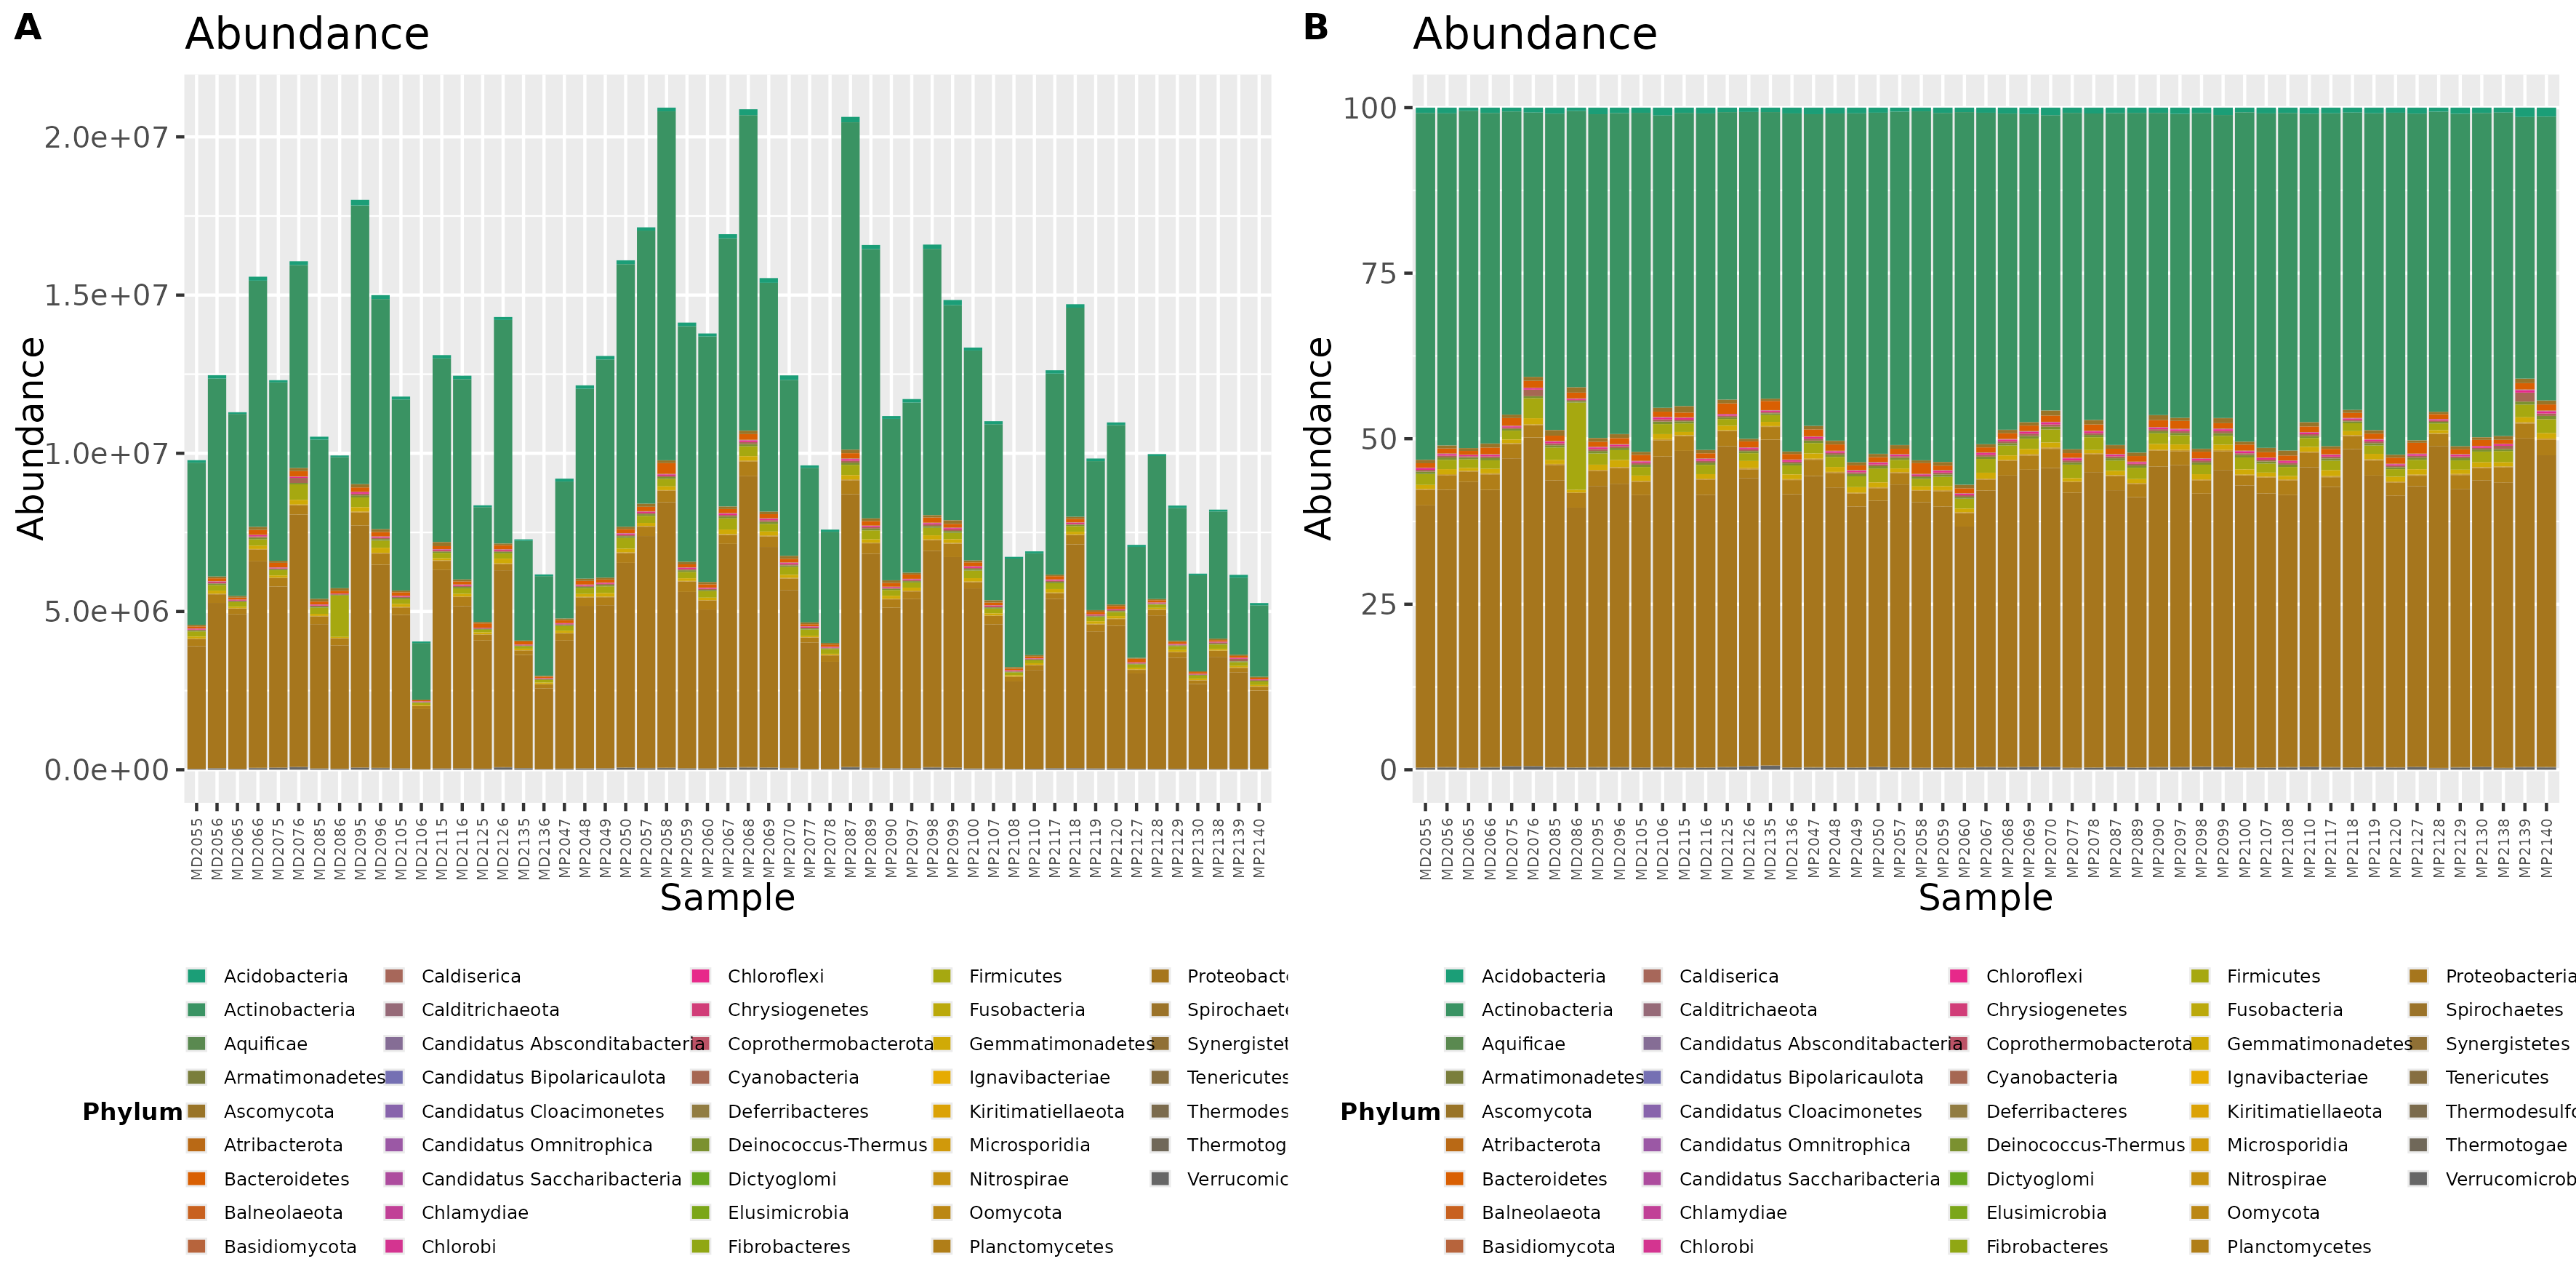
\includegraphics[width=\textwidth]{Img/cap2/filo_plot.png}
\caption{A)Barras de abundancias absolutas y B) relativas a nivel de filo}
\end{figure}
Podemos notar algunas diferencias entre los diferentes filos; sin embargo, la gran cantidad de taxones dificulta distinguir adecuadamente el color de cada uno, a menos que tengan una abundancia muy significativa. Dado que nuestro objetivo es diferenciar entre muestras sanas y enfermas, agregaremos una distinción adicional utilizando la variable 'Tratamiento': representaremos las muestras sanas en color blanco y las muestras enfermas en color negro.\\
\begin{figure}[h]
\centering
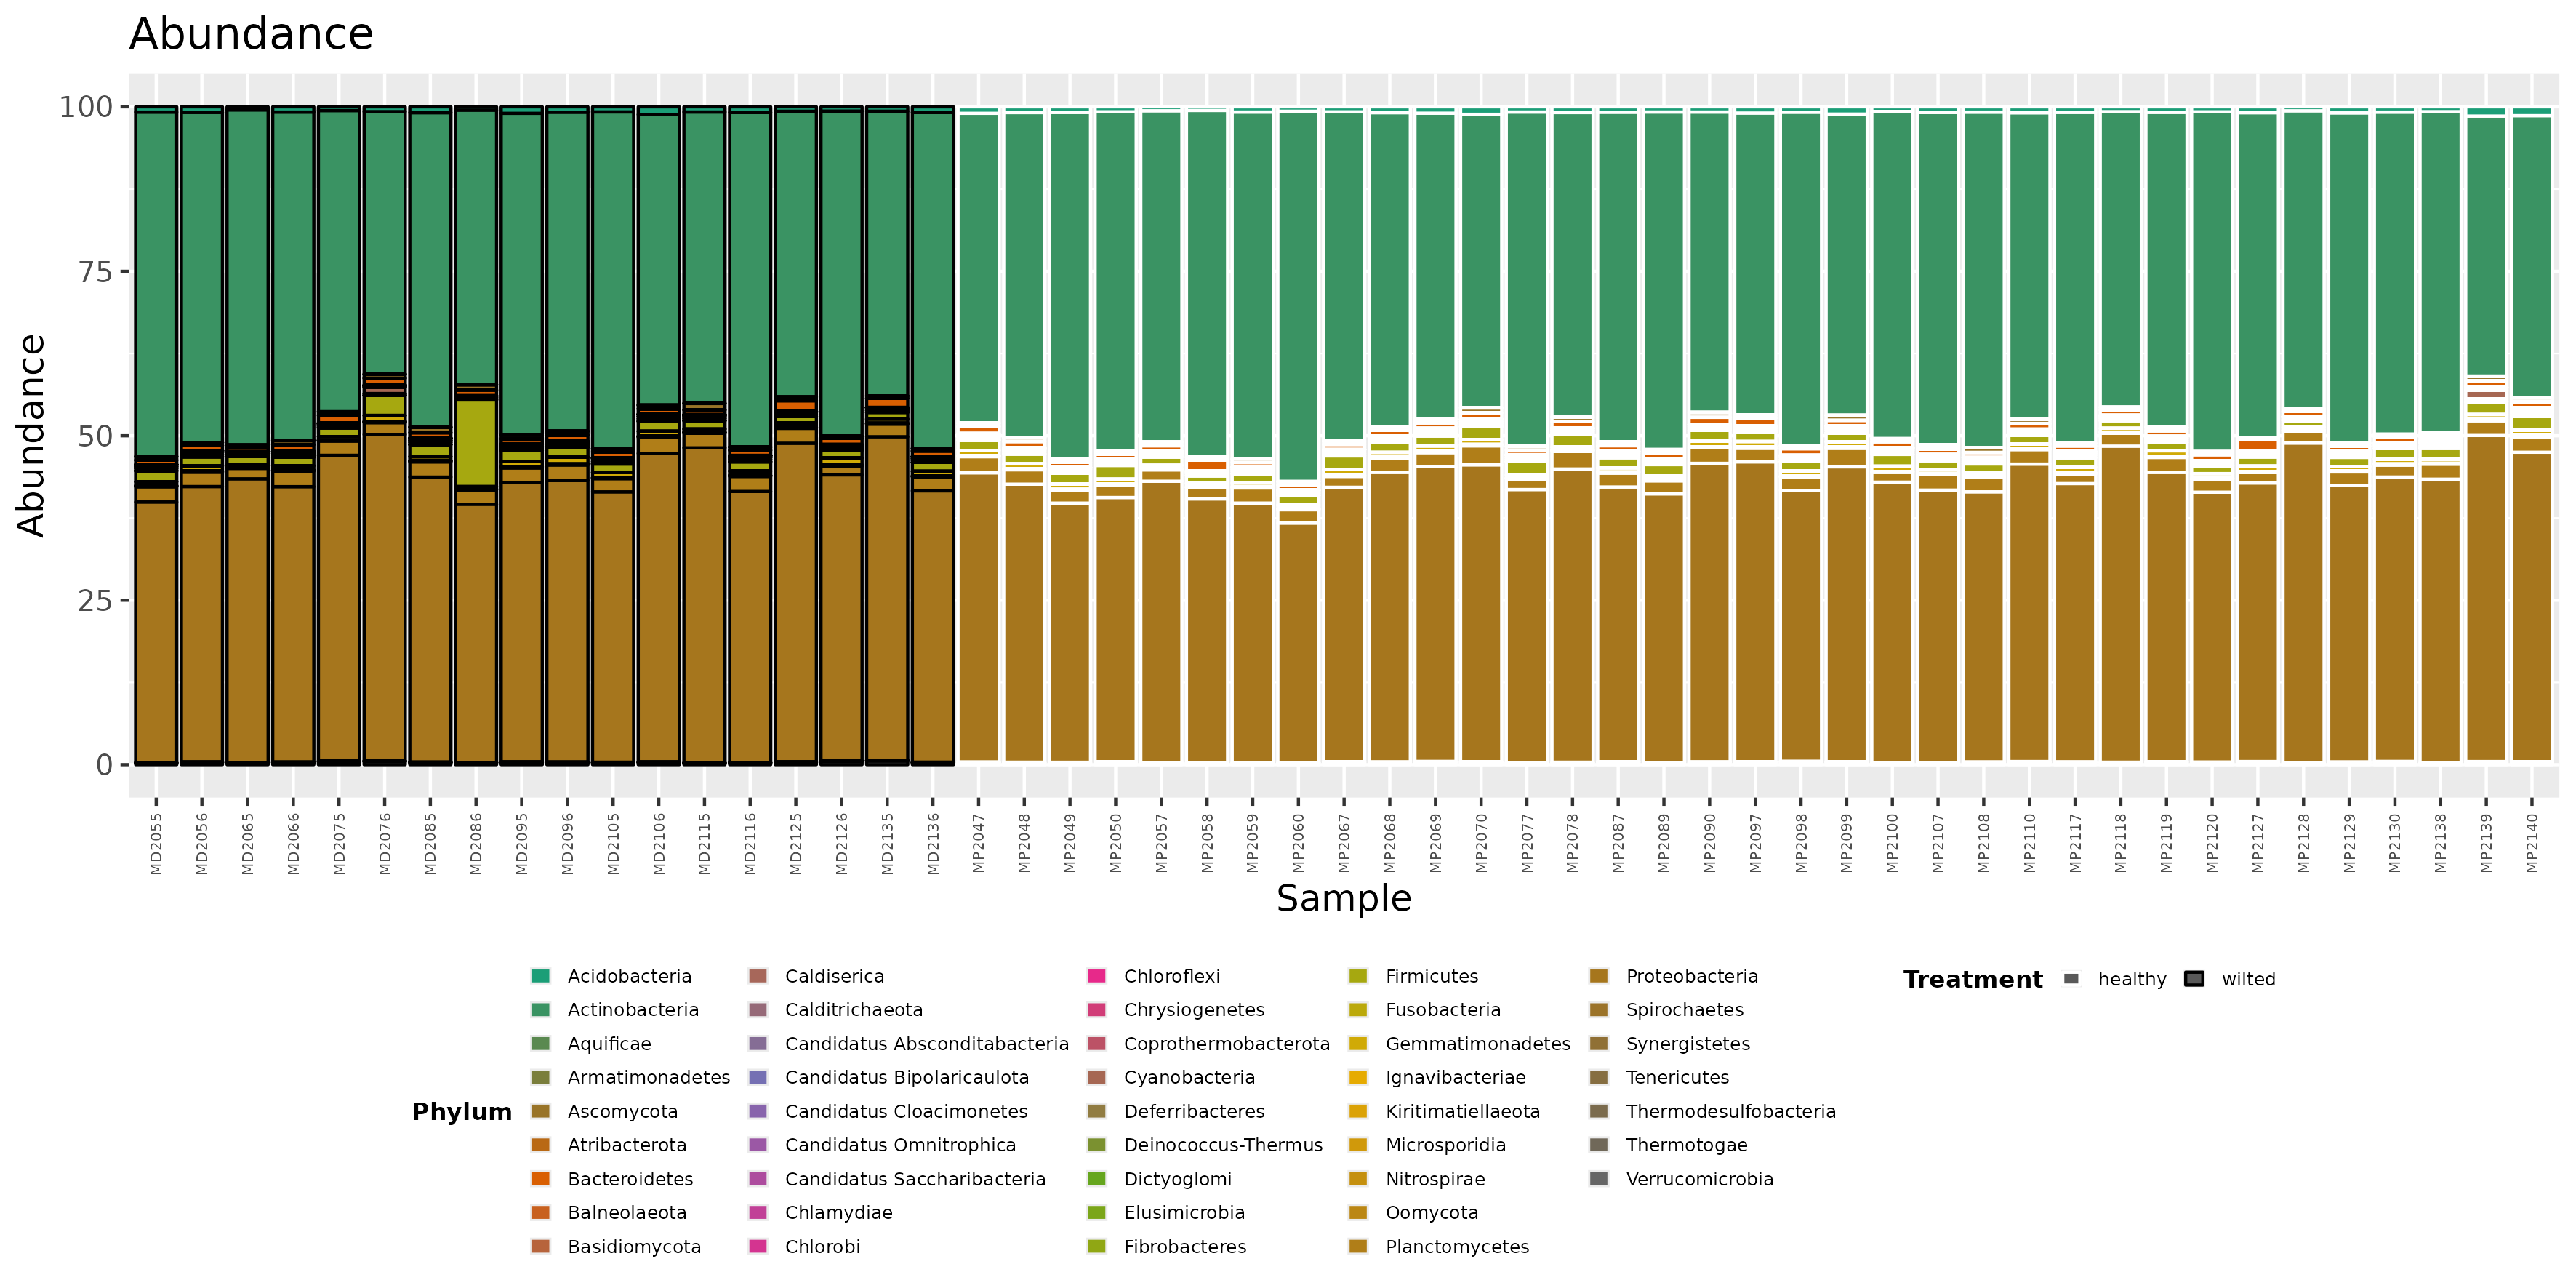
\includegraphics[width=\textwidth]{Img/cap2/filo_plot_blackandwhite.png}
\caption{Barras de abundancias relativas separando entre sanas y enfermas}
\end{figure}
De igual manera, la cantidad de taxones dificulta la distinción entre las muestras. Por ello, hemos creado subconjuntos más pequeños para facilitar una observación más clara de nuestros datos.\\

En el análisis de diversos grupos taxonómicos, comenzamos examinando gráficos de barras de abundancias como primer paso para seleccionar conjuntos específicos de interés. Al representar las muestras en el eje x y las abundancias en el eje y, obtenemos una visualización clara de las abundancias absolutas y relativas en cada muestra. Este enfoque nos facilita identificar de manera eficiente conjuntos particulares que pueden ser fundamentales para un análisis más detallado y específico.\\

Basándonos en los resultados y medidas anteriores, procedemos a explorar las muestras a diferentes niveles taxonómicos específicos, comenzando con los subconjuntos a nivel de reino, en este caso, Bacteria y Eucariota.\\

Podemos ver cuantos “Eukaryota” tenemos en “Kingdom”.
\begin{lstlisting}[basicstyle=\small] 
sum(fresa_kraken_fil@tax_table@.Data[,"Kingdom"]=="Eukaryota")
## [1] 181
\end{lstlisting}
\begin{lstlisting}[basicstyle=\small] 
sum(fresa_kraken_fil@tax_table@.Data[,"Kingdom"]=="Bacteria")
## [1] 8822
\end{lstlisting}

Al verificar lo observado anteriormente con la agrupación de subconjuntos, confirmamos que hay una mayor cantidad de muestras clasificadas como bacterias en comparación con las clasificadas como eucariotas.\\

A partir de estos dos subconjuntos, llevamos a cabo una agrupación adicional por filo, familia, género y especie. La elección de estos niveles taxonómicos se basa en diferentes propósitos: el filo se selecciona como el siguiente nivel después del reino para proporcionar una visualización panorámica de los datos; mientras que la familia, el género y la especie se seleccionan para obtener una visualización más detallada y poder identificar diferencias significativas entre los grupos de datos.\\

\textbf{GLOM10\%}
Se realiza una aglomeracion al diez por ciento (10\%)  para tener una mejor visibilidad y podernos enfocar en las muestras con menor (mayor) abundancia. \\

\begin{figure}[h]
\centering
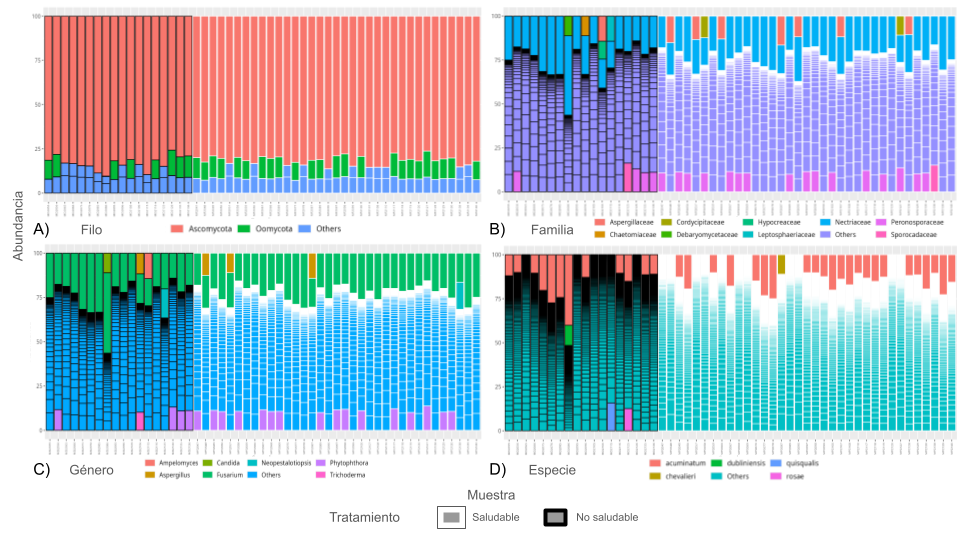
\includegraphics[width=\textwidth]{Img/cap2/Barras_Eukarya10.png}
\caption{Barras de abundancia para eucariota a nivel A) Filo, B) Familia, C) Genero, D) Especie,  \href{https://github.com/CamilaSilva1995/Tesis_Maestria/blob/main/Analisis_Comparativo/Fresa_Solena/20230227_Funciones&Graficas.R}{(FuncionesGraficas.R)}}
\end{figure}

\begin{figure}[h]
\centering
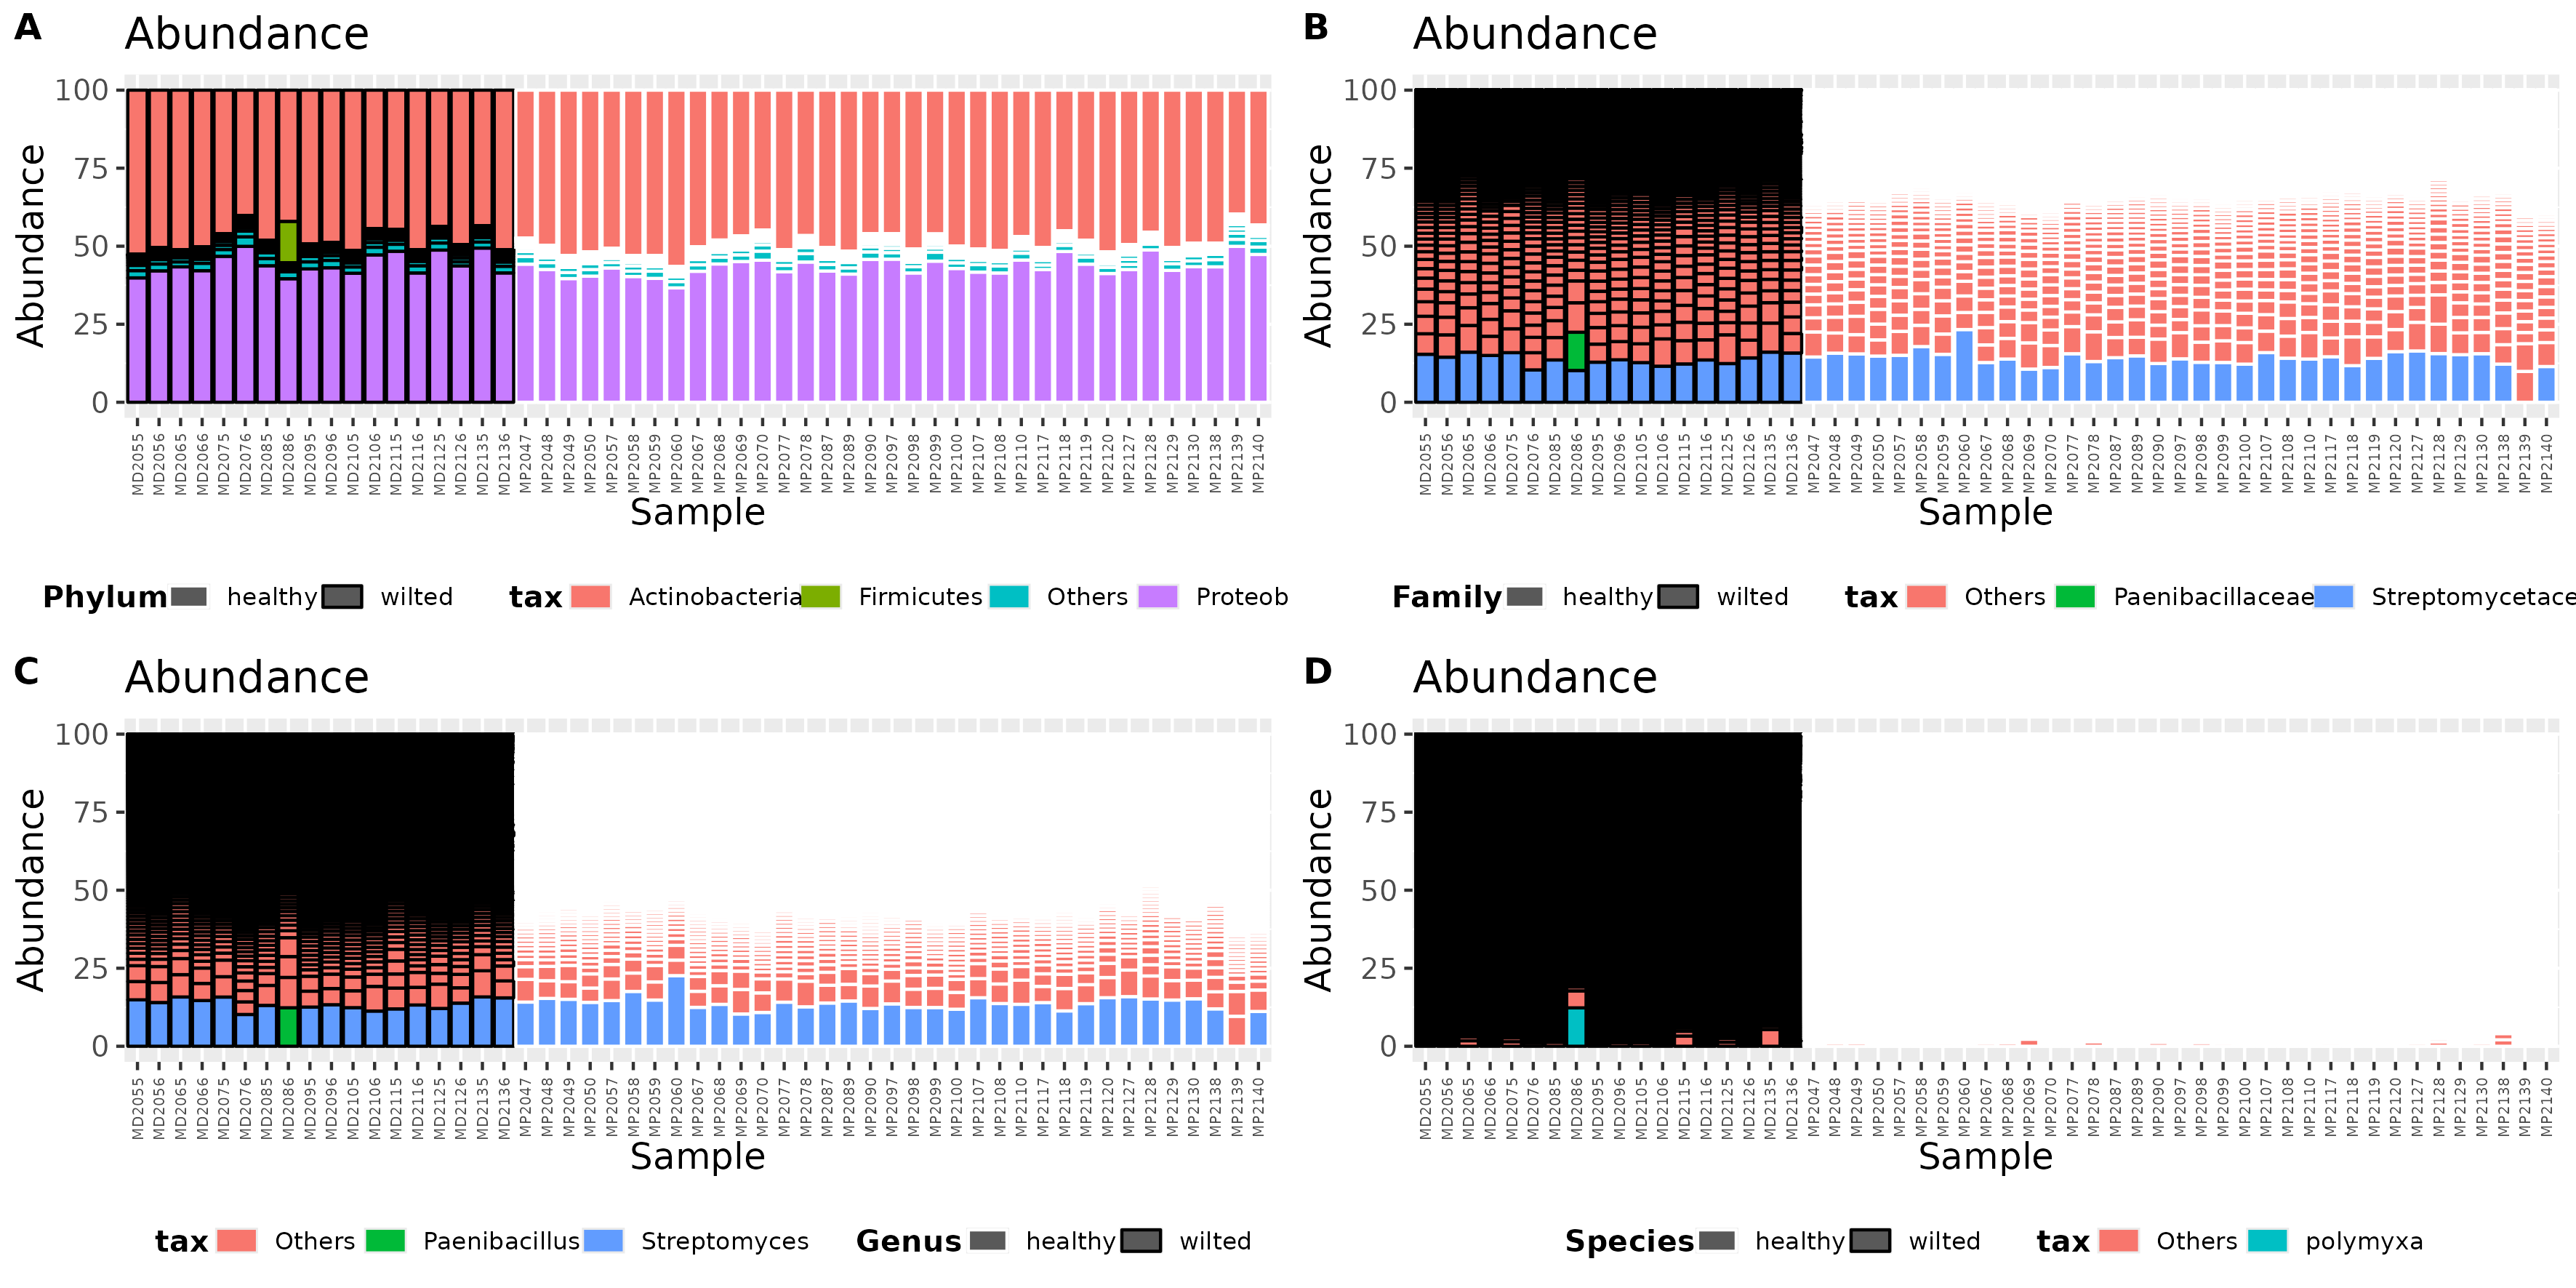
\includegraphics[width=\textwidth]{Img/cap2/Barras_Bacteria10.png}
\caption{Barras de abundancia para bacteria a nivel A) Filo, B) Familia, C) Genero, D) Especie, \href{https://github.com/CamilaSilva1995/Tesis_Maestria/blob/main/Analisis_Comparativo/Fresa_Solena/20230227_Funciones&Graficas.R}{(FuncionesGraficas.R)}}
\end{figure}

En esta representación a nivel de filo, podemos destacar la disminución notable de \textit{Oomycota} en las muestras enfermas en comparación con las muestras sanas. Al profundizar a nivel de familia, observamos una disminución específica de \textit{Peronosporaceae} en las muestras enfermas en comparación con las muestras sanas.\\

\textbf{Diversidad alfa para los niveles taxonomicos}

\begin{figure}[h]
\centering
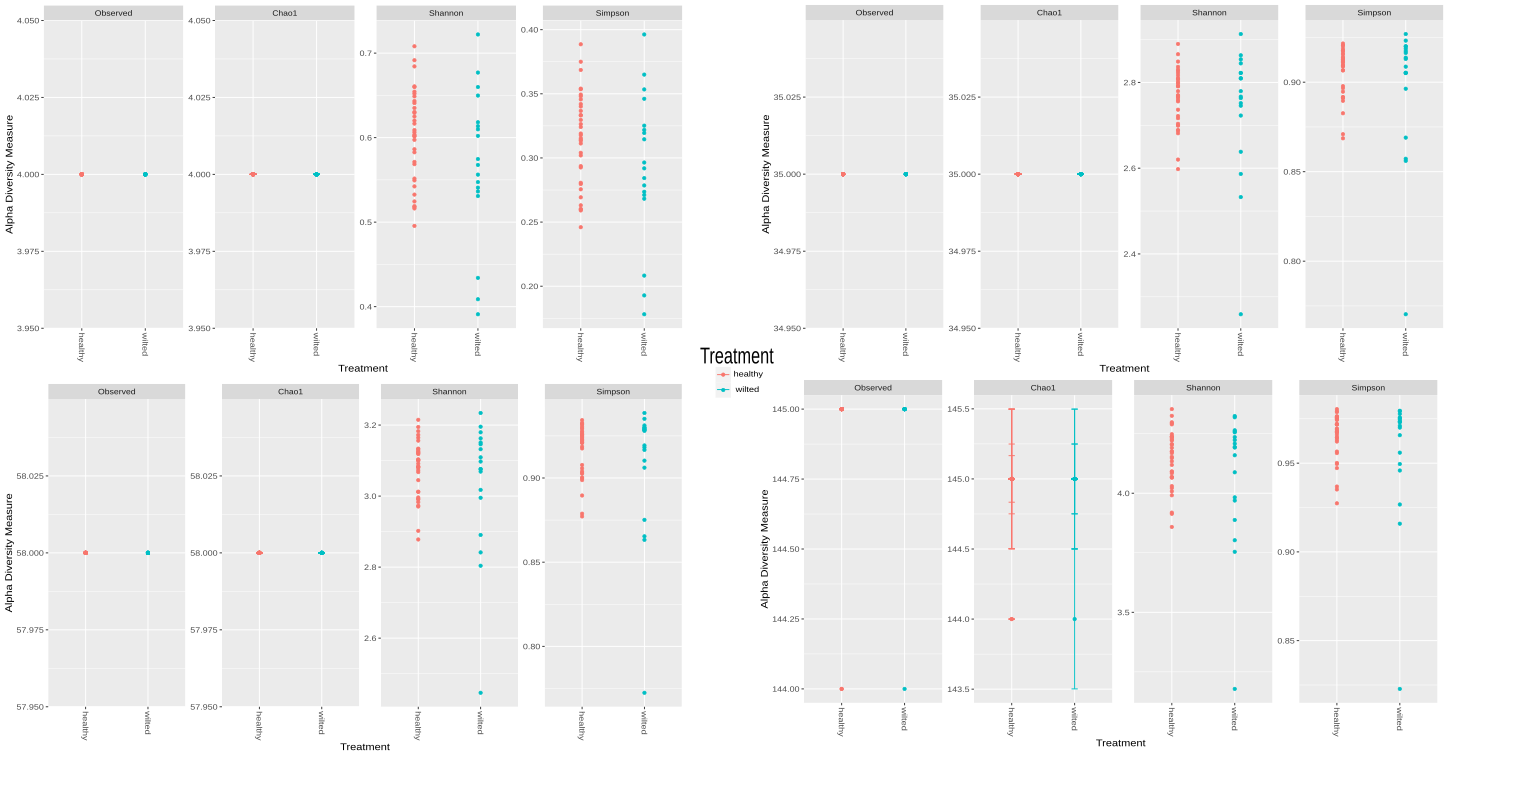
\includegraphics[width=\textwidth]{Img/cap2/Alpha_Eukarya.png}
\caption{Diversidad alpha para eucariota a nivel de A) Filo, B) Familia, C) Genero, D) Especie \href{https://github.com/CamilaSilva1995/Tesis_Maestria/blob/main/Analisis_Comparativo/Fresa_Solena/20230227_Funciones&Graficas.R}{(FuncionesGraficas.R)}}
\end{figure}
En esta imagen, podemos ver que con la diversidad Chao1 a nivel de especie se genera una diferencia considerable de diversidades entre muestras sanas y enfermas, lo cual se detallara mas adelante con una prueba de hipótesis. Tambien ...
\begin{figure}[h]
\centering
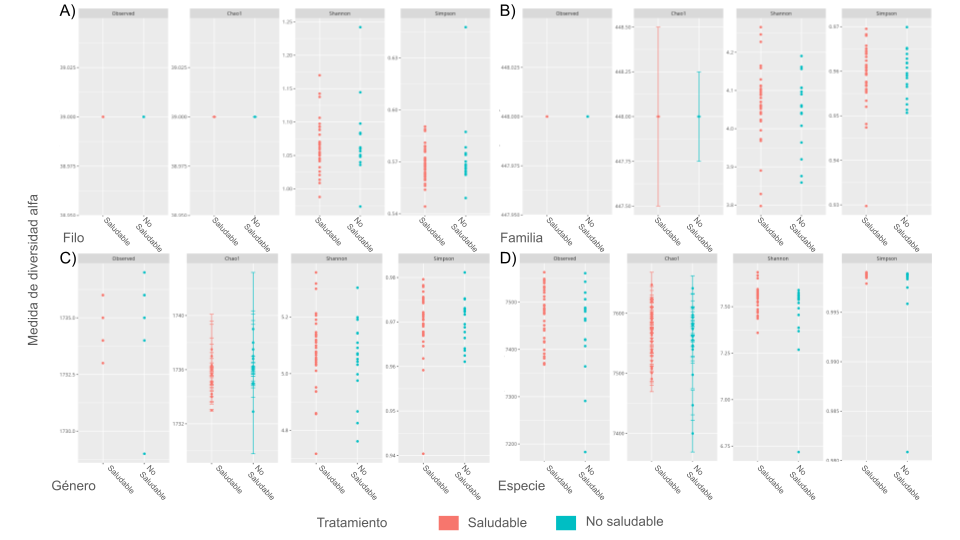
\includegraphics[width=\textwidth]{Img/cap2/Alpha_Bacteria.png}
\caption{Diversidad alpha para bacteria a nivel de A) Filo, B) Familia, C) Genero, D) Especie \href{https://github.com/CamilaSilva1995/Tesis_Maestria/blob/main/Analisis_Comparativo/Fresa_Solena/20230227_Funciones&Graficas.R}{(FuncionesGraficas.R)}}
\end{figure}
En esta imagen, podemos ver que con la diversidad Chao1 a nivel de género se evidencia una diferencia considerable de diversidades entre muestras sanas y enfermas, lo cual se detallara mas adelante con una prueba de hipótesis. Tambien ...

\textbf{Diversidad beta para los niveles taxonomicos}

\begin{figure}[h]
\centering
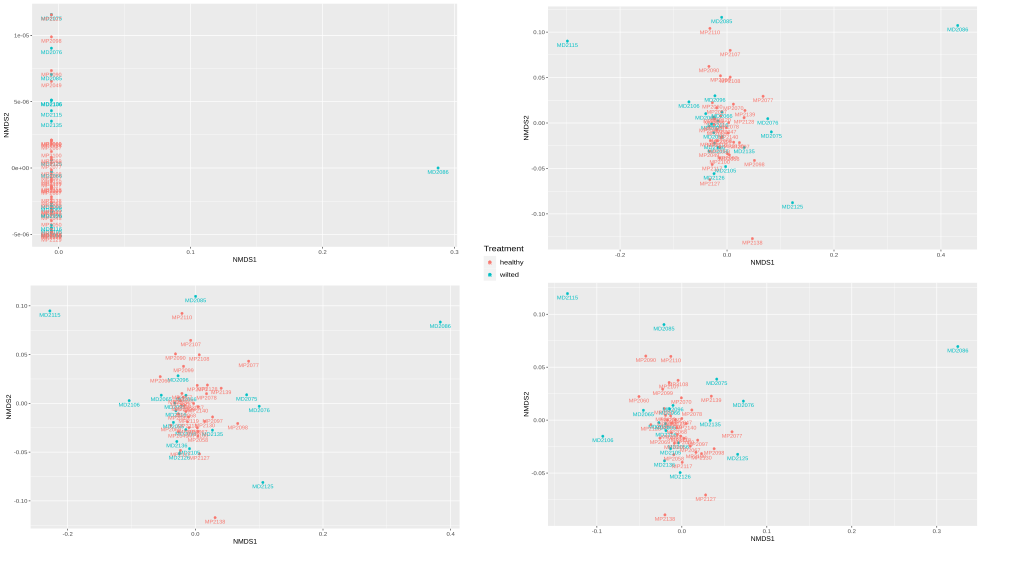
\includegraphics[width=\textwidth]{Img/cap2/Beta_Eukarya.png}
\caption{Diversidad beta para eucariota a nivel de A) Filo, B) Familia, C) Genero, D) Especie \href{https://github.com/CamilaSilva1995/Tesis_Maestria/blob/main/Analisis_Comparativo/Fresa_Solena/20230227_Funciones&Graficas.R}{(FuncionesGraficas.R)}}
\end{figure}

\begin{figure}[h]
\centering
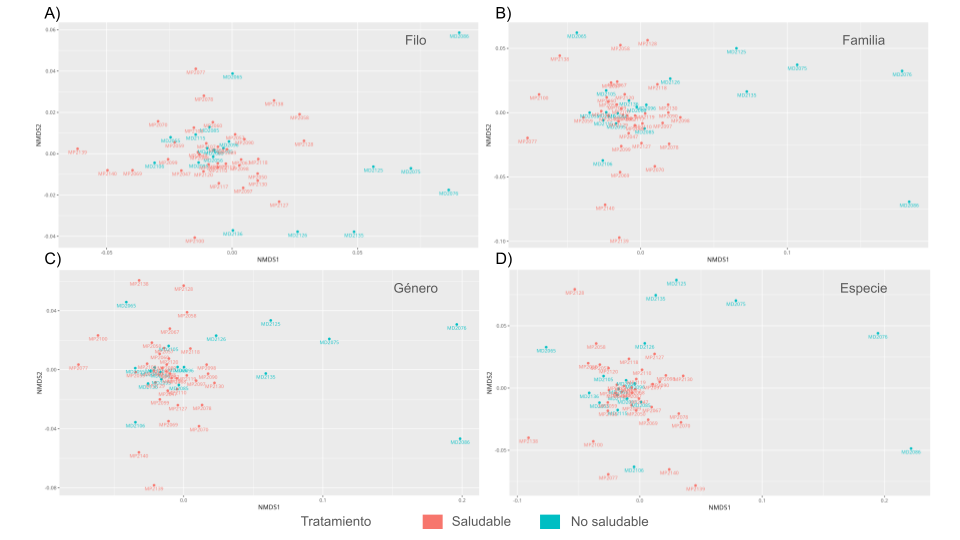
\includegraphics[width=\textwidth]{Img/cap2/Beta_Bacteria.png}
\caption{Diversidad beta para bacteria a nivel de A) Filo, B) Familia, C) Genero, D) Especie \href{https://github.com/CamilaSilva1995/Tesis_Maestria/blob/main/Analisis_Comparativo/Fresa_Solena/20230227_Funciones&Graficas.R}{(FuncionesGraficas.R)}}
\end{figure}


\section{Prueba de Hipótesis}
La hipótesis es una suposición sobre los datos, la cual puede resultar verdadera o falsa..\\

Las pruebas de hipótesis son herramientas valiosas en diversos campos, ya que permiten contrastar una teoría con la evidencia empírica. Este procedimiento riguroso nos ayuda a evaluar la veracidad de una afirmación científica de manera objetiva y fundamentada. En esencia, una prueba de hipótesis se define como un método estadístico que se emplea para tomar decisiones sobre una población en base a los datos obtenidos de una muestra representativa. Es una técnica de inferencia estadística que nos permite tomar decisiones sobre suposiciones acerca de una población, basadas en la observación.\\

El propósito de una prueba estadística es examinar una hipótesis con respecto a los valores de uno o más parámetros poblacionales. Los componentes de una prueba estadística incluyen: la hipótesis nula, la hipótesis alternativa, el estadístico de prueba, la región de rechazo y el valor p. \\
\textbf{Hipótesis nula ($H_0$):} Es la idea inicial, la suposición que se pone a prueba. Representa la creencia de que no hay diferencia o efecto significativo.\\
\textbf{Hipótesis alternativa ($H_1$): }Es la contrapropuesta, lo que se espera encontrar si la $H_0$ es falsa. Representa la alternativa que se busca demostrar.\\
\textbf{Estadístico de prueba: }Es la herramienta matemática (funcionde las mediciones muestrales) que utilizamos para analizar los datos y determinar si apoyan o no la $H_1$. Cada prueba estadística tiene su propio estadístico específico.\\
\textbf{Región de rechazo: }Es una zona predefinida como territorio prohibido para la $H_0$. Si el valor del estadístico de prueba cae en esta región, la $H_0$ se rechaza por considerarse poco probable. ($x$ es el valor critico observado, el cual define la region de rechazo)\\
\textbf{ P-valor:} Es la probabilidad de obtener un valor del estadístico de prueba tan extremo o más extremo que el observado, suponiendo que la $H_0$ sea verdadera. Un valor de p bajo (menor que el nivel de significancia $\alpha $  el cual se fija previamente  ) indica que es poco probable que el resultado se deba al azar, lo que lleva al rechazo de la $H_0$.\\

En donde el objetivo principal de esta prueba es rechazar la hipótesis nula.\\

\begin{figure}[h]
\centering
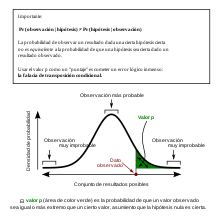
\includegraphics[width=\textwidth]{Img/cap2/pvalor.png}
\caption{imagen de ejemplo p-valor}
\end{figure}

El p\-valor se considera como una medida de la probabilidad de éxito (obtener un resultado específico) en un estudio estadístico con los datos observados. El cálculo de este valor depende de la prueba estadística utilizada y de las suposiciones realizadas sobre la distribución de los datos. En general, un valor pequeño del p-valor sugiere que los datos observados son poco probables bajo la hipótesis nula.\\
%Rice, J. A. (2006). Mathematical Statistics and Data Analysis (3rd ed.)
%Wasserman, L. (2004). All of Statistics: A Concise Course in Statistical Inference.
A continuación, se realizan las siguientes pruebas de hipótesis, todas basadas en esta premisa, pero aplicadas a diferentes medidas de los datos. \\
	

\subsection{Pruebas con muestras pequeñas para comparar dos medias poblacionales}

Suponemos dos poblaciones independientes con distibuciones normales con 

$$\sigma_{1}^{2} = \sigma_{2}^{2}$$

y queremos probar (tenemos como hipotesis nula)

$$H_{0} : \mu_{1} = \mu _{2}$$

respecto a la hipotesis alternativa

$$H_{a} : \mu_{1} \neq \mu _{2}$$

tomando como estadistico de prueba:

$$ T = \frac{\bar{Y_{1}} - \bar{Y_{2}}}{S_{p}\sqrt{\frac{1}{n_{1}} + \frac{1}{n_{2}}}}$$

donde  

$$ S_{p} = \sqrt{\frac{(n_{1}-1)S_{1}^{2} + (n_{2}-1)S_{2}^{2}}{n_{1} + n_{2} - 2}}$$

\begin{figure}[!]
\centering
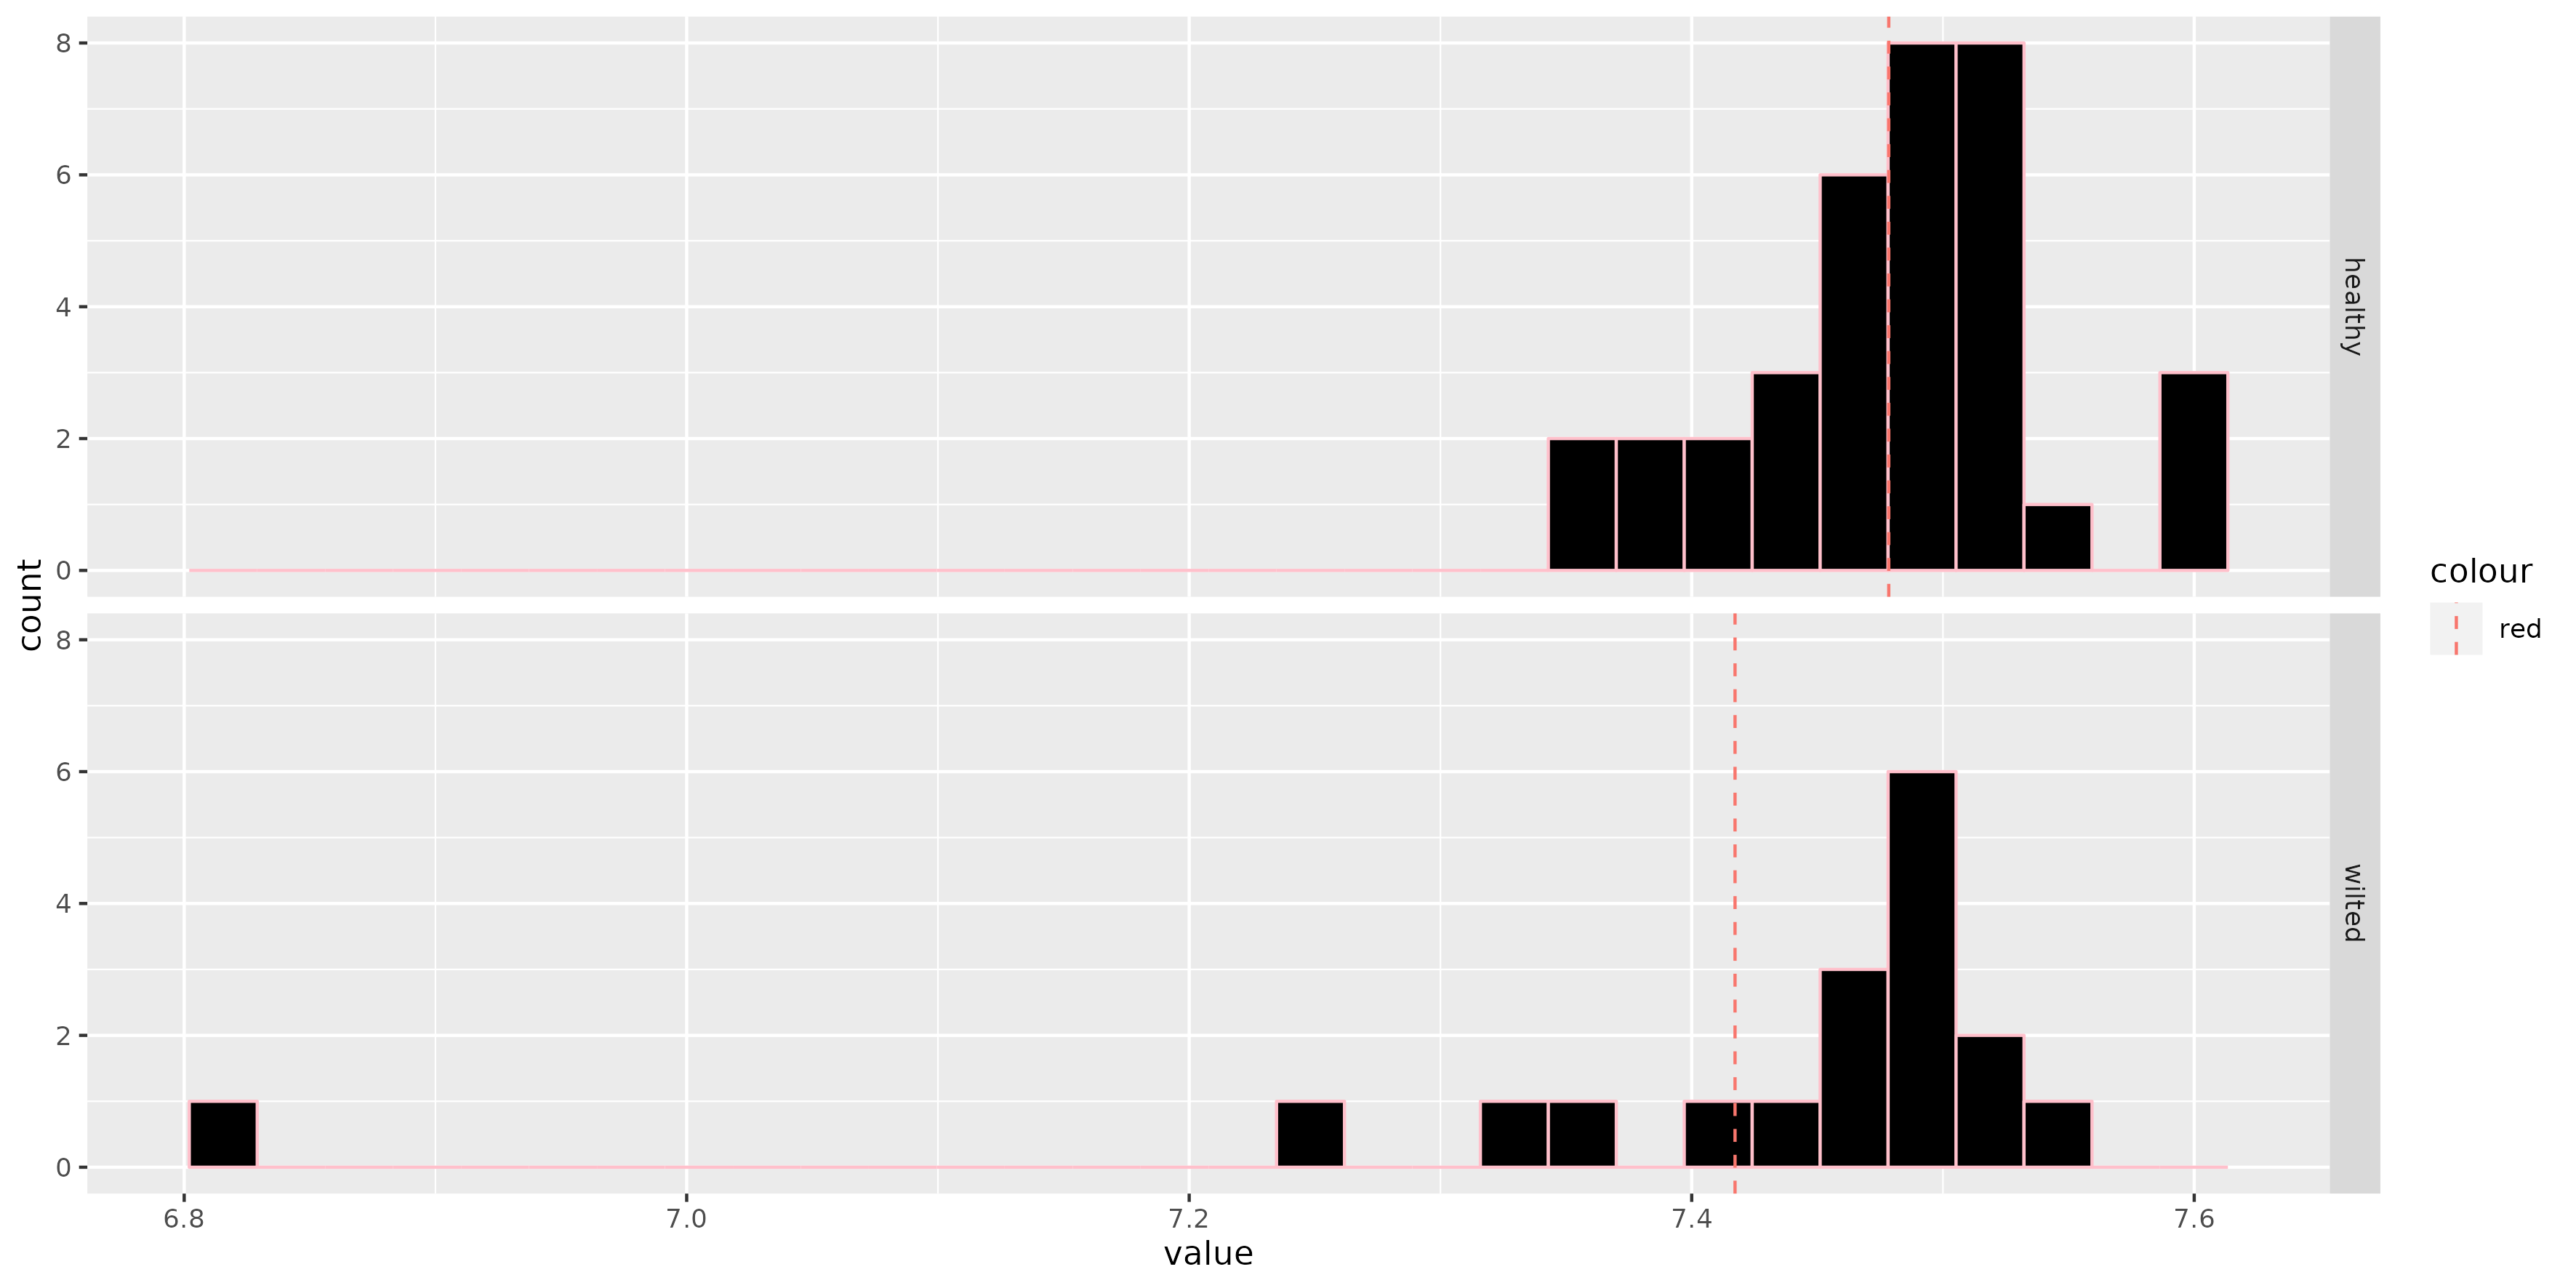
\includegraphics[width=\textwidth]{Img/cap2/medias_Shannon.png}
\caption{}
\end{figure}

\begin{figure}[!]
\centering
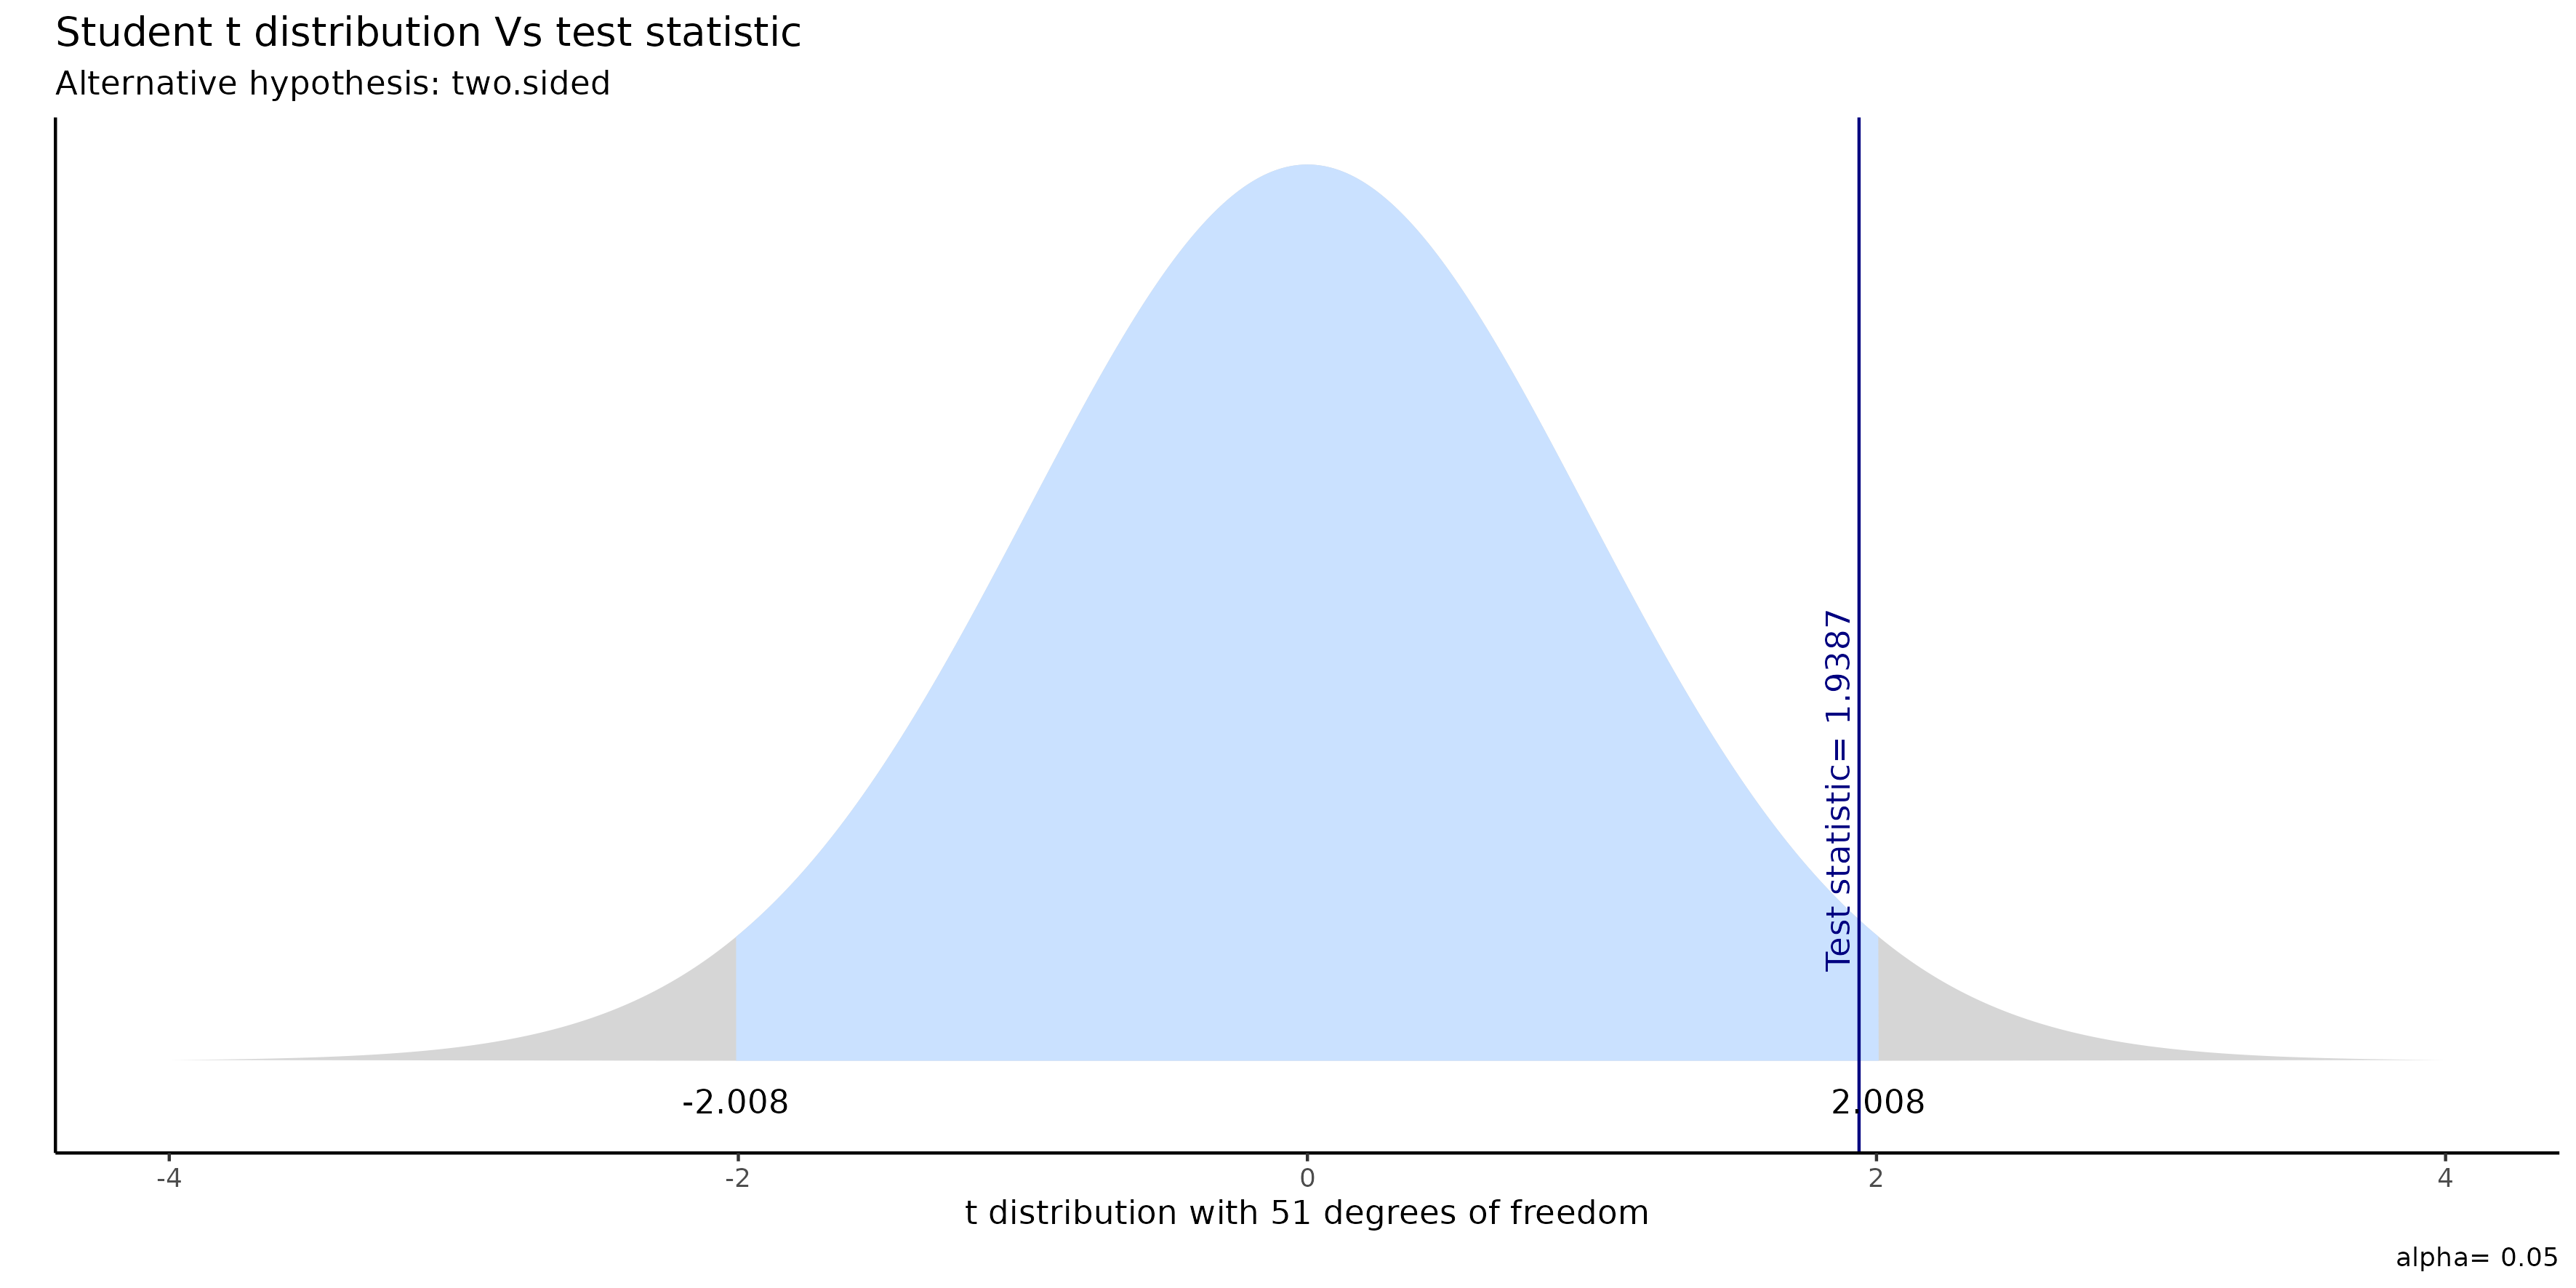
\includegraphics[width=\textwidth]{Img/cap2/pruebat_varianzasiguales_Shannon.png}
\caption{}
\end{figure}

\begin{figure}[!]
\centering
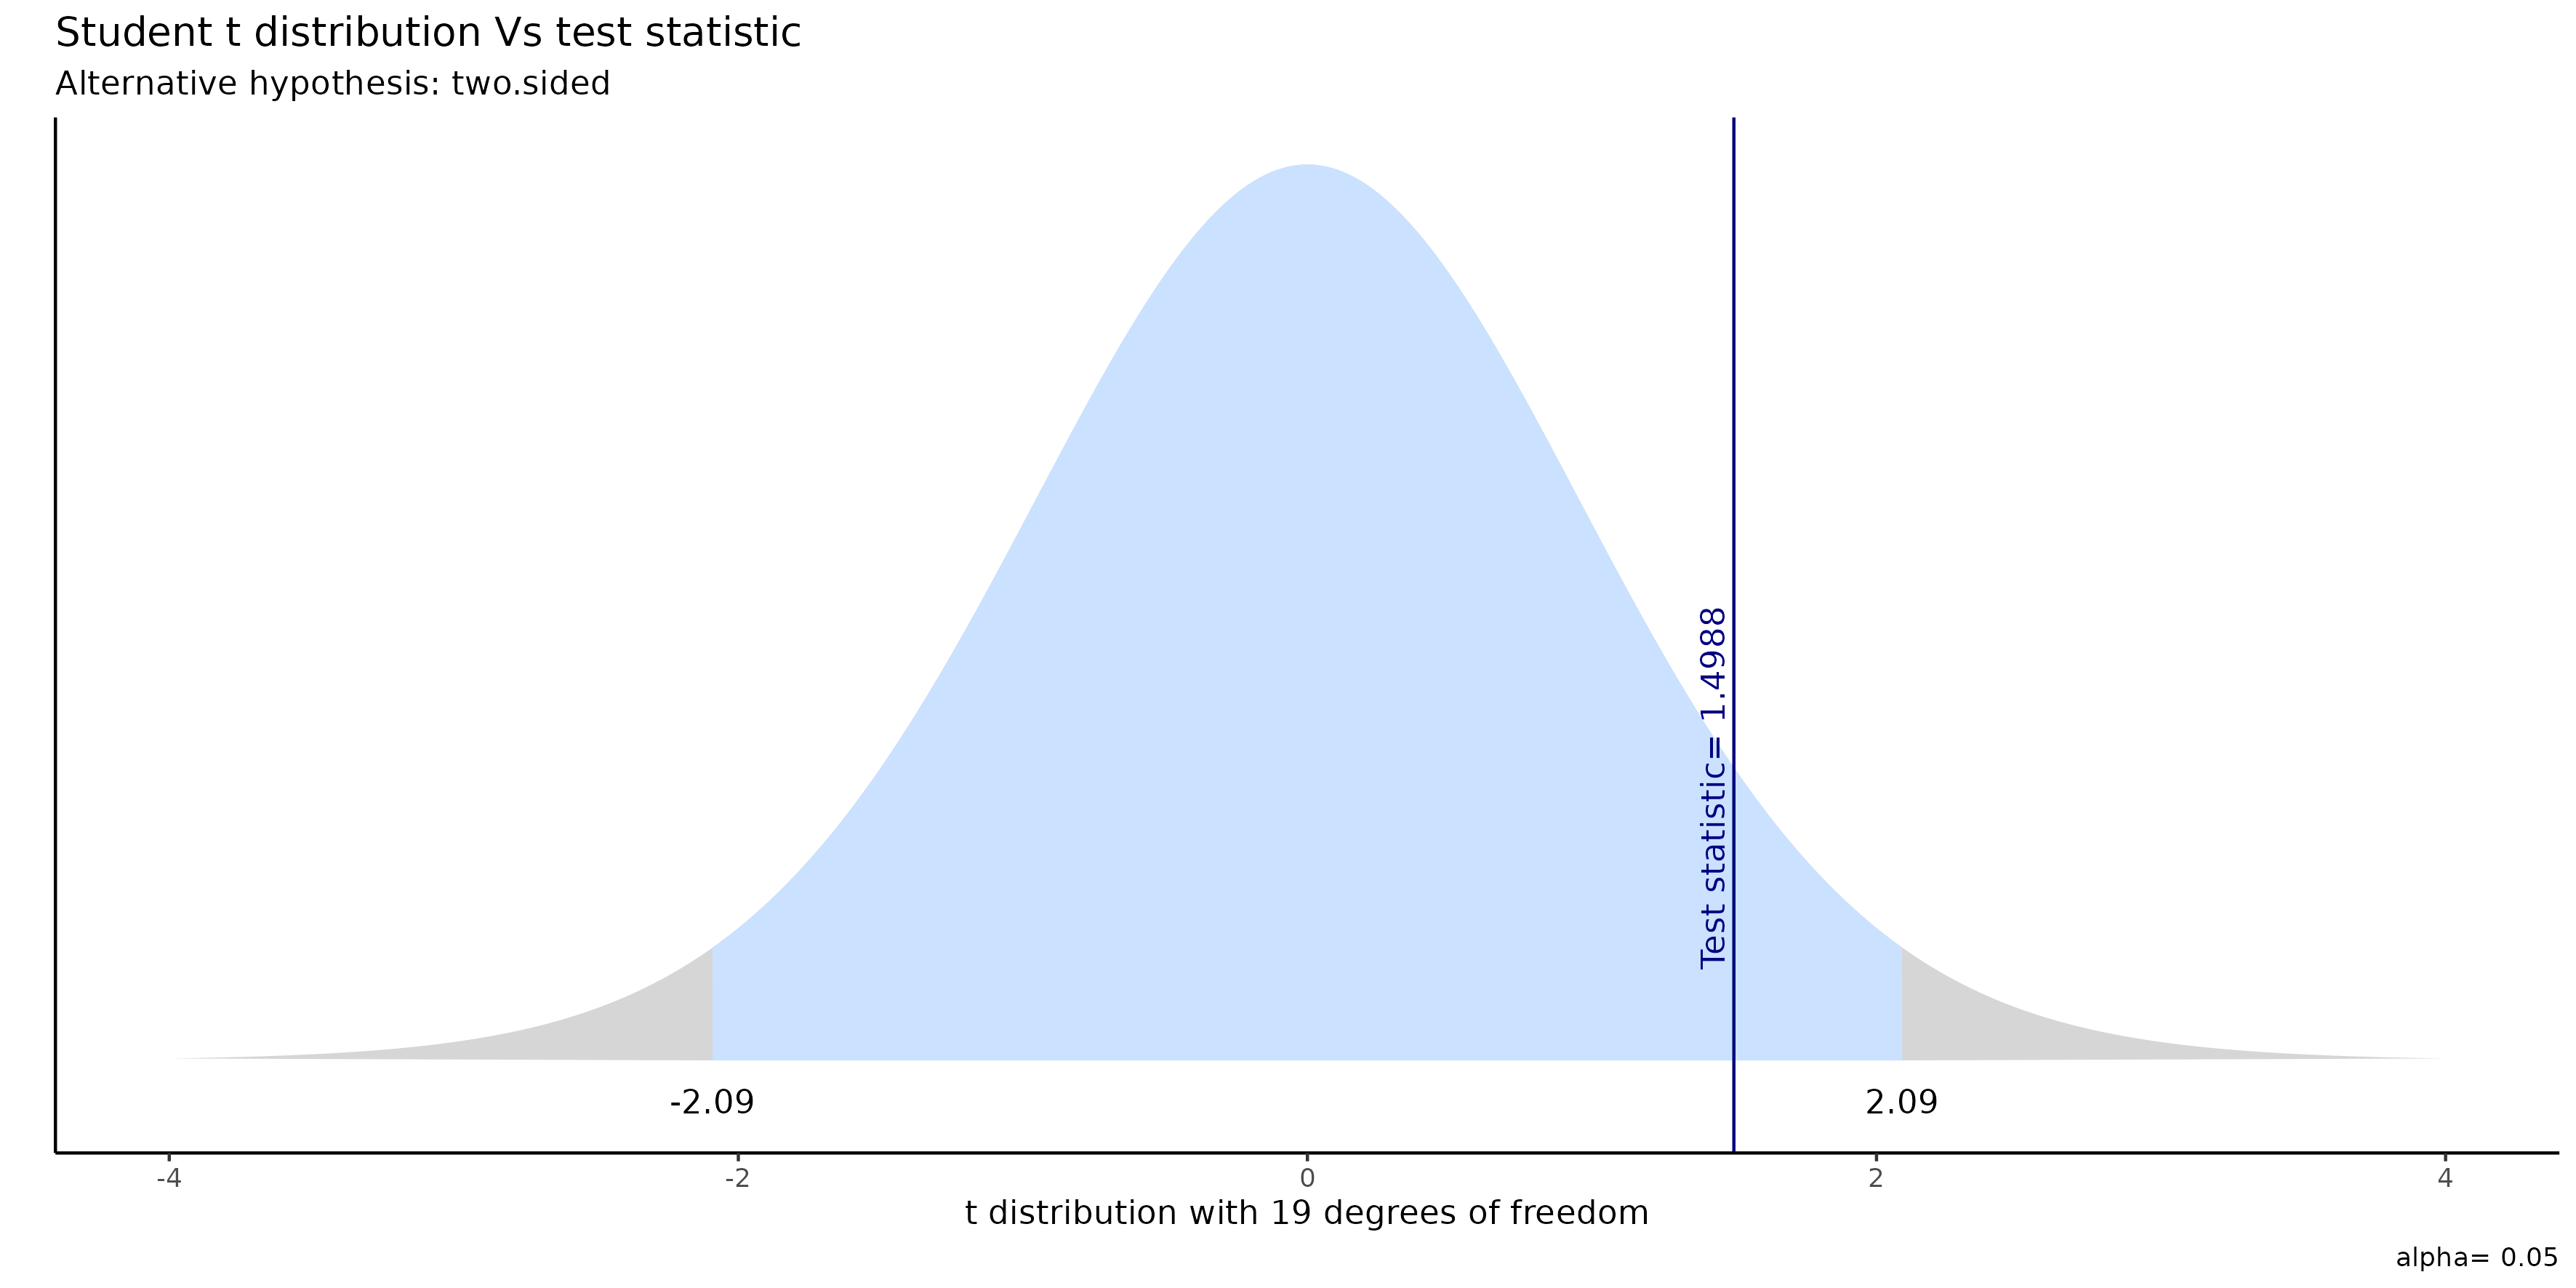
\includegraphics[width=\textwidth]{Img/cap2/pruebat_varianzasdiferentes_Shannon.png}
\caption{}
\end{figure}


\begin{figure}[!]
\centering
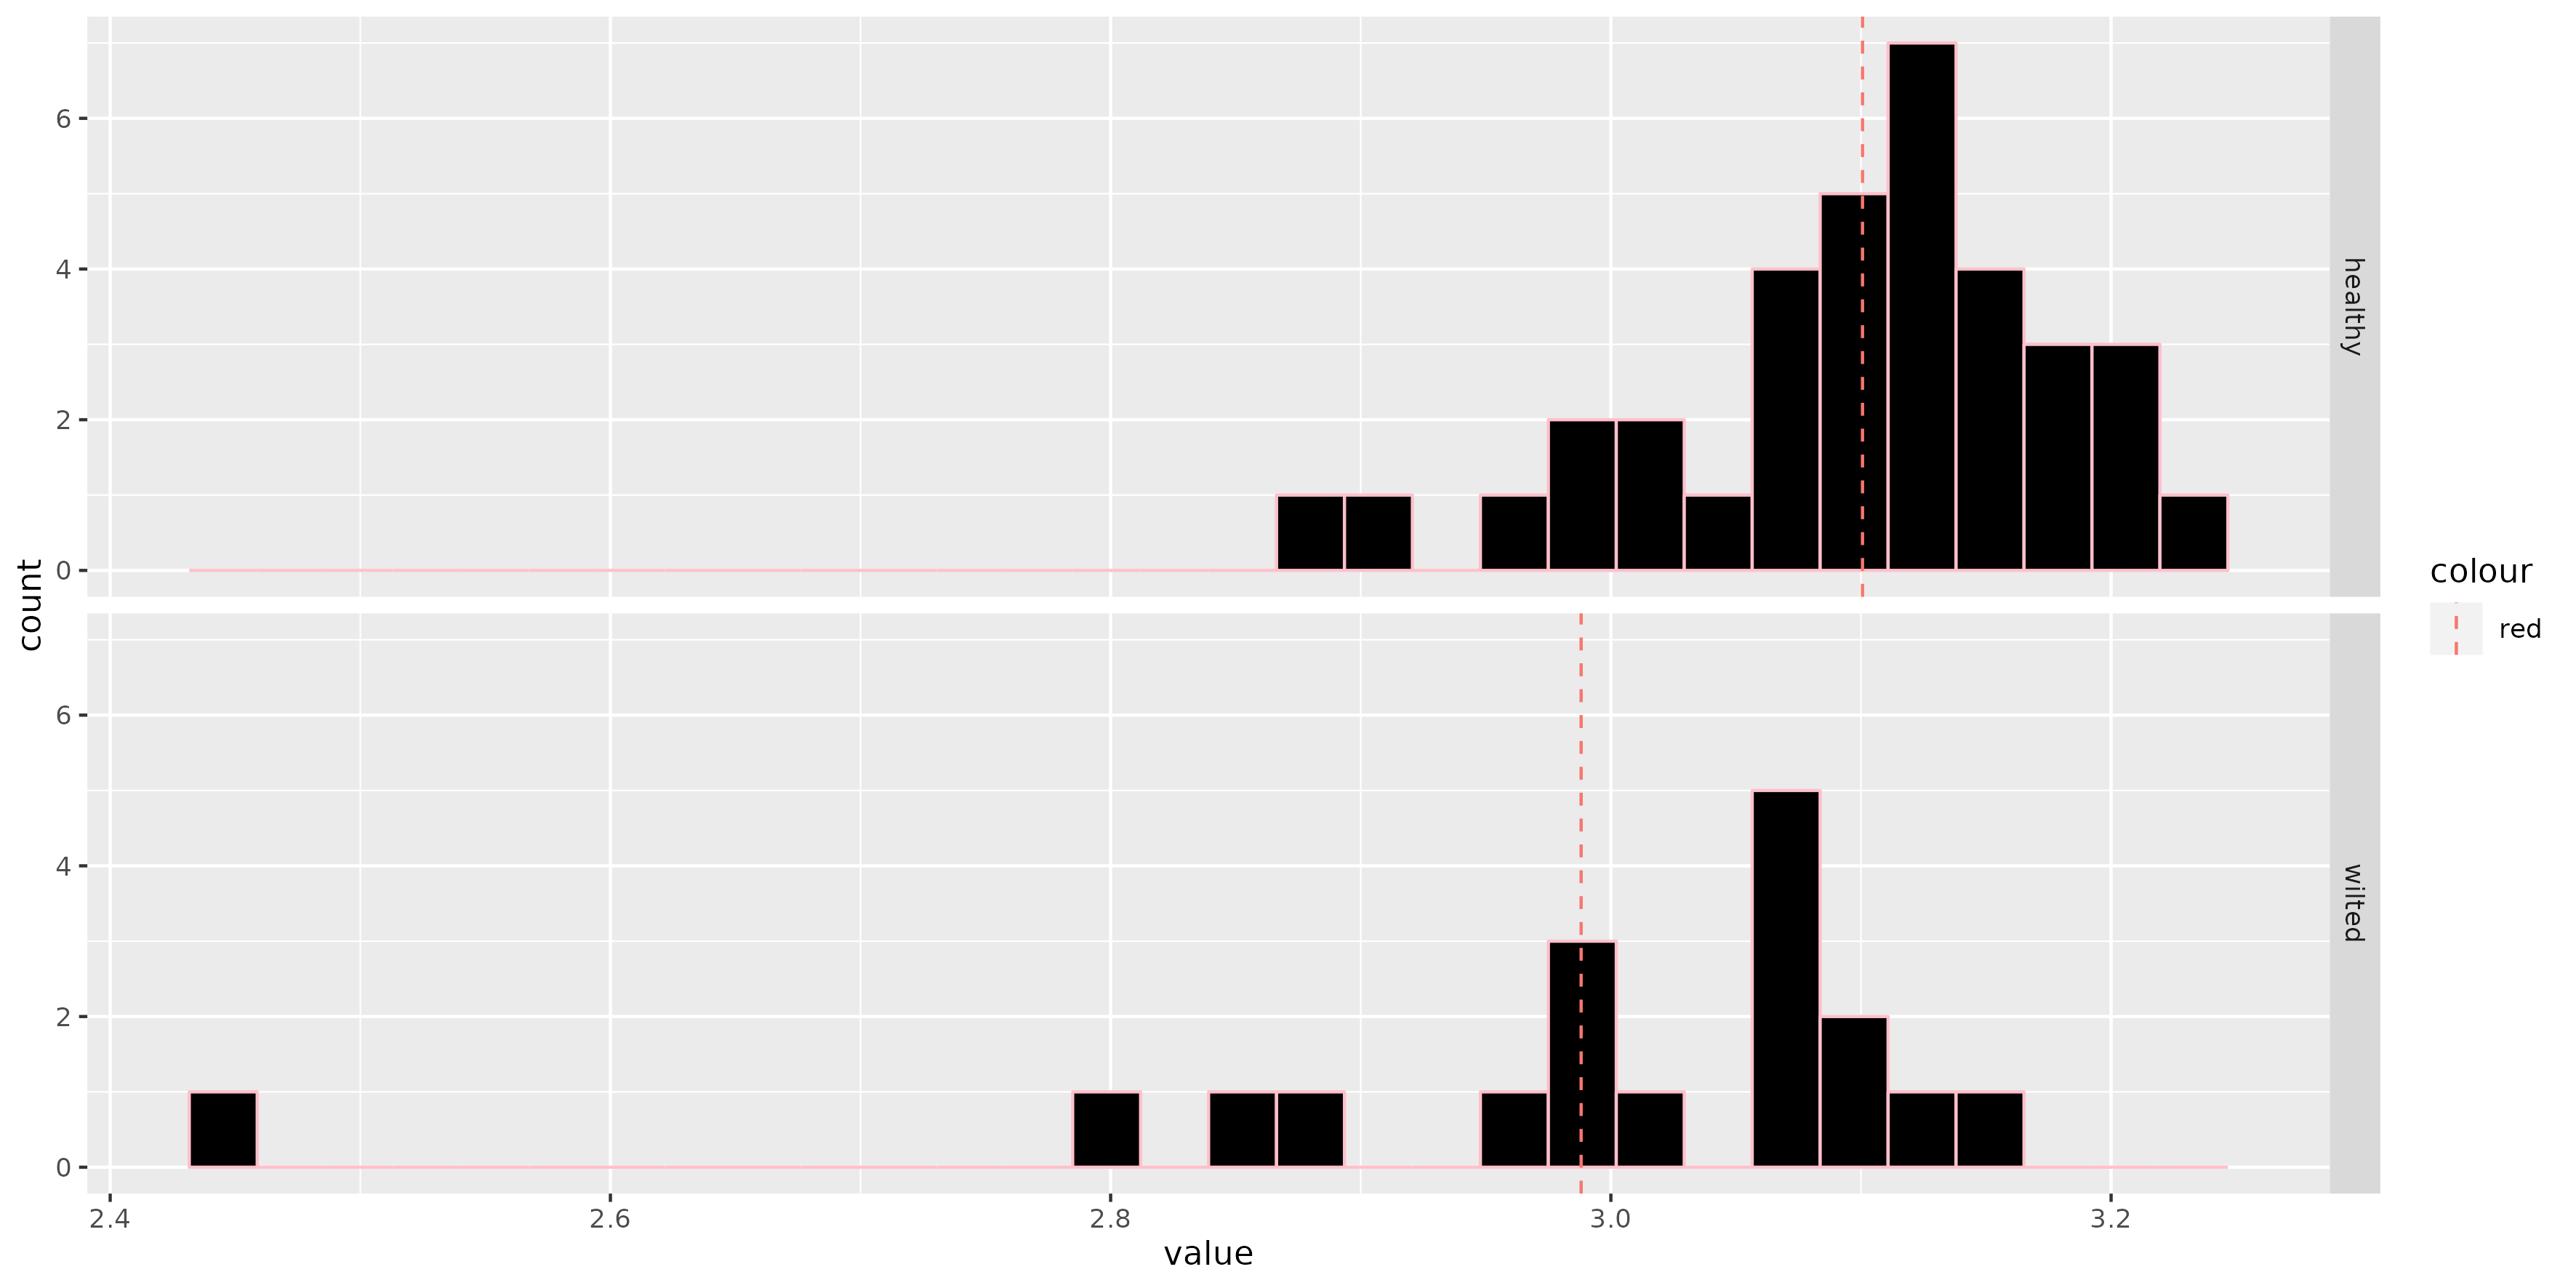
\includegraphics[width=\textwidth]{Img/cap2/mediasFusarium_Shannon.png}
\caption{}
\end{figure}

\begin{figure}[!]
\centering
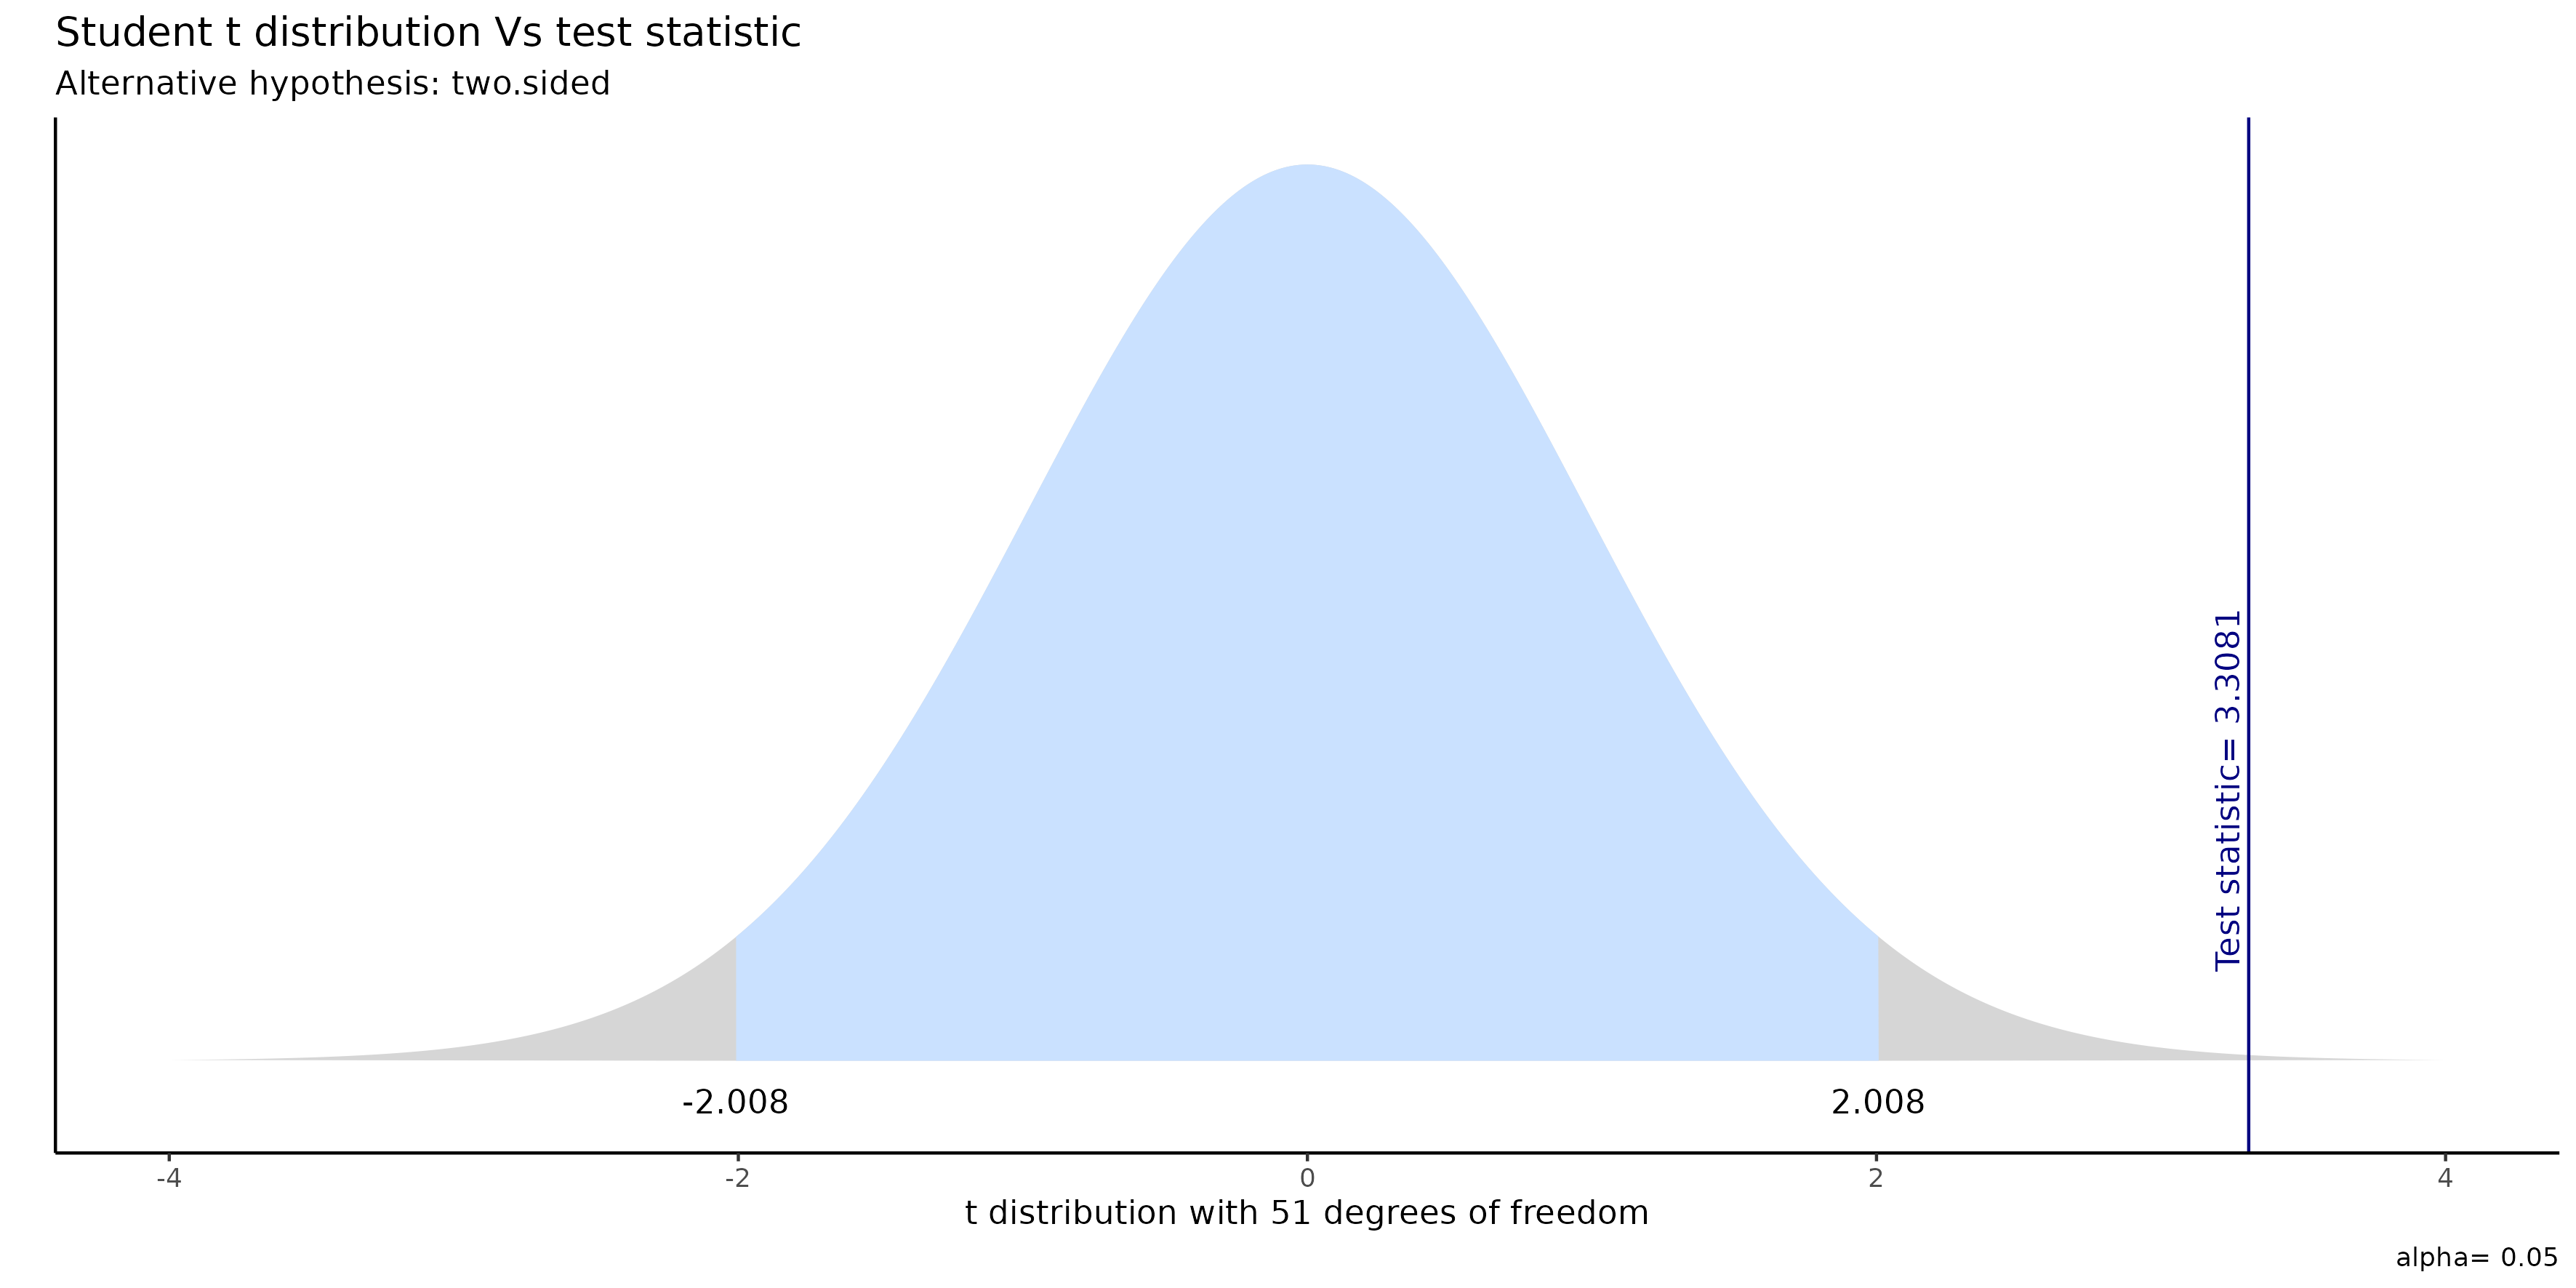
\includegraphics[width=\textwidth]{Img/cap2/pruebat_varianzasigualesFusarium_Shannon.png}
\caption{}
\end{figure}

\begin{figure}[!]
\centering
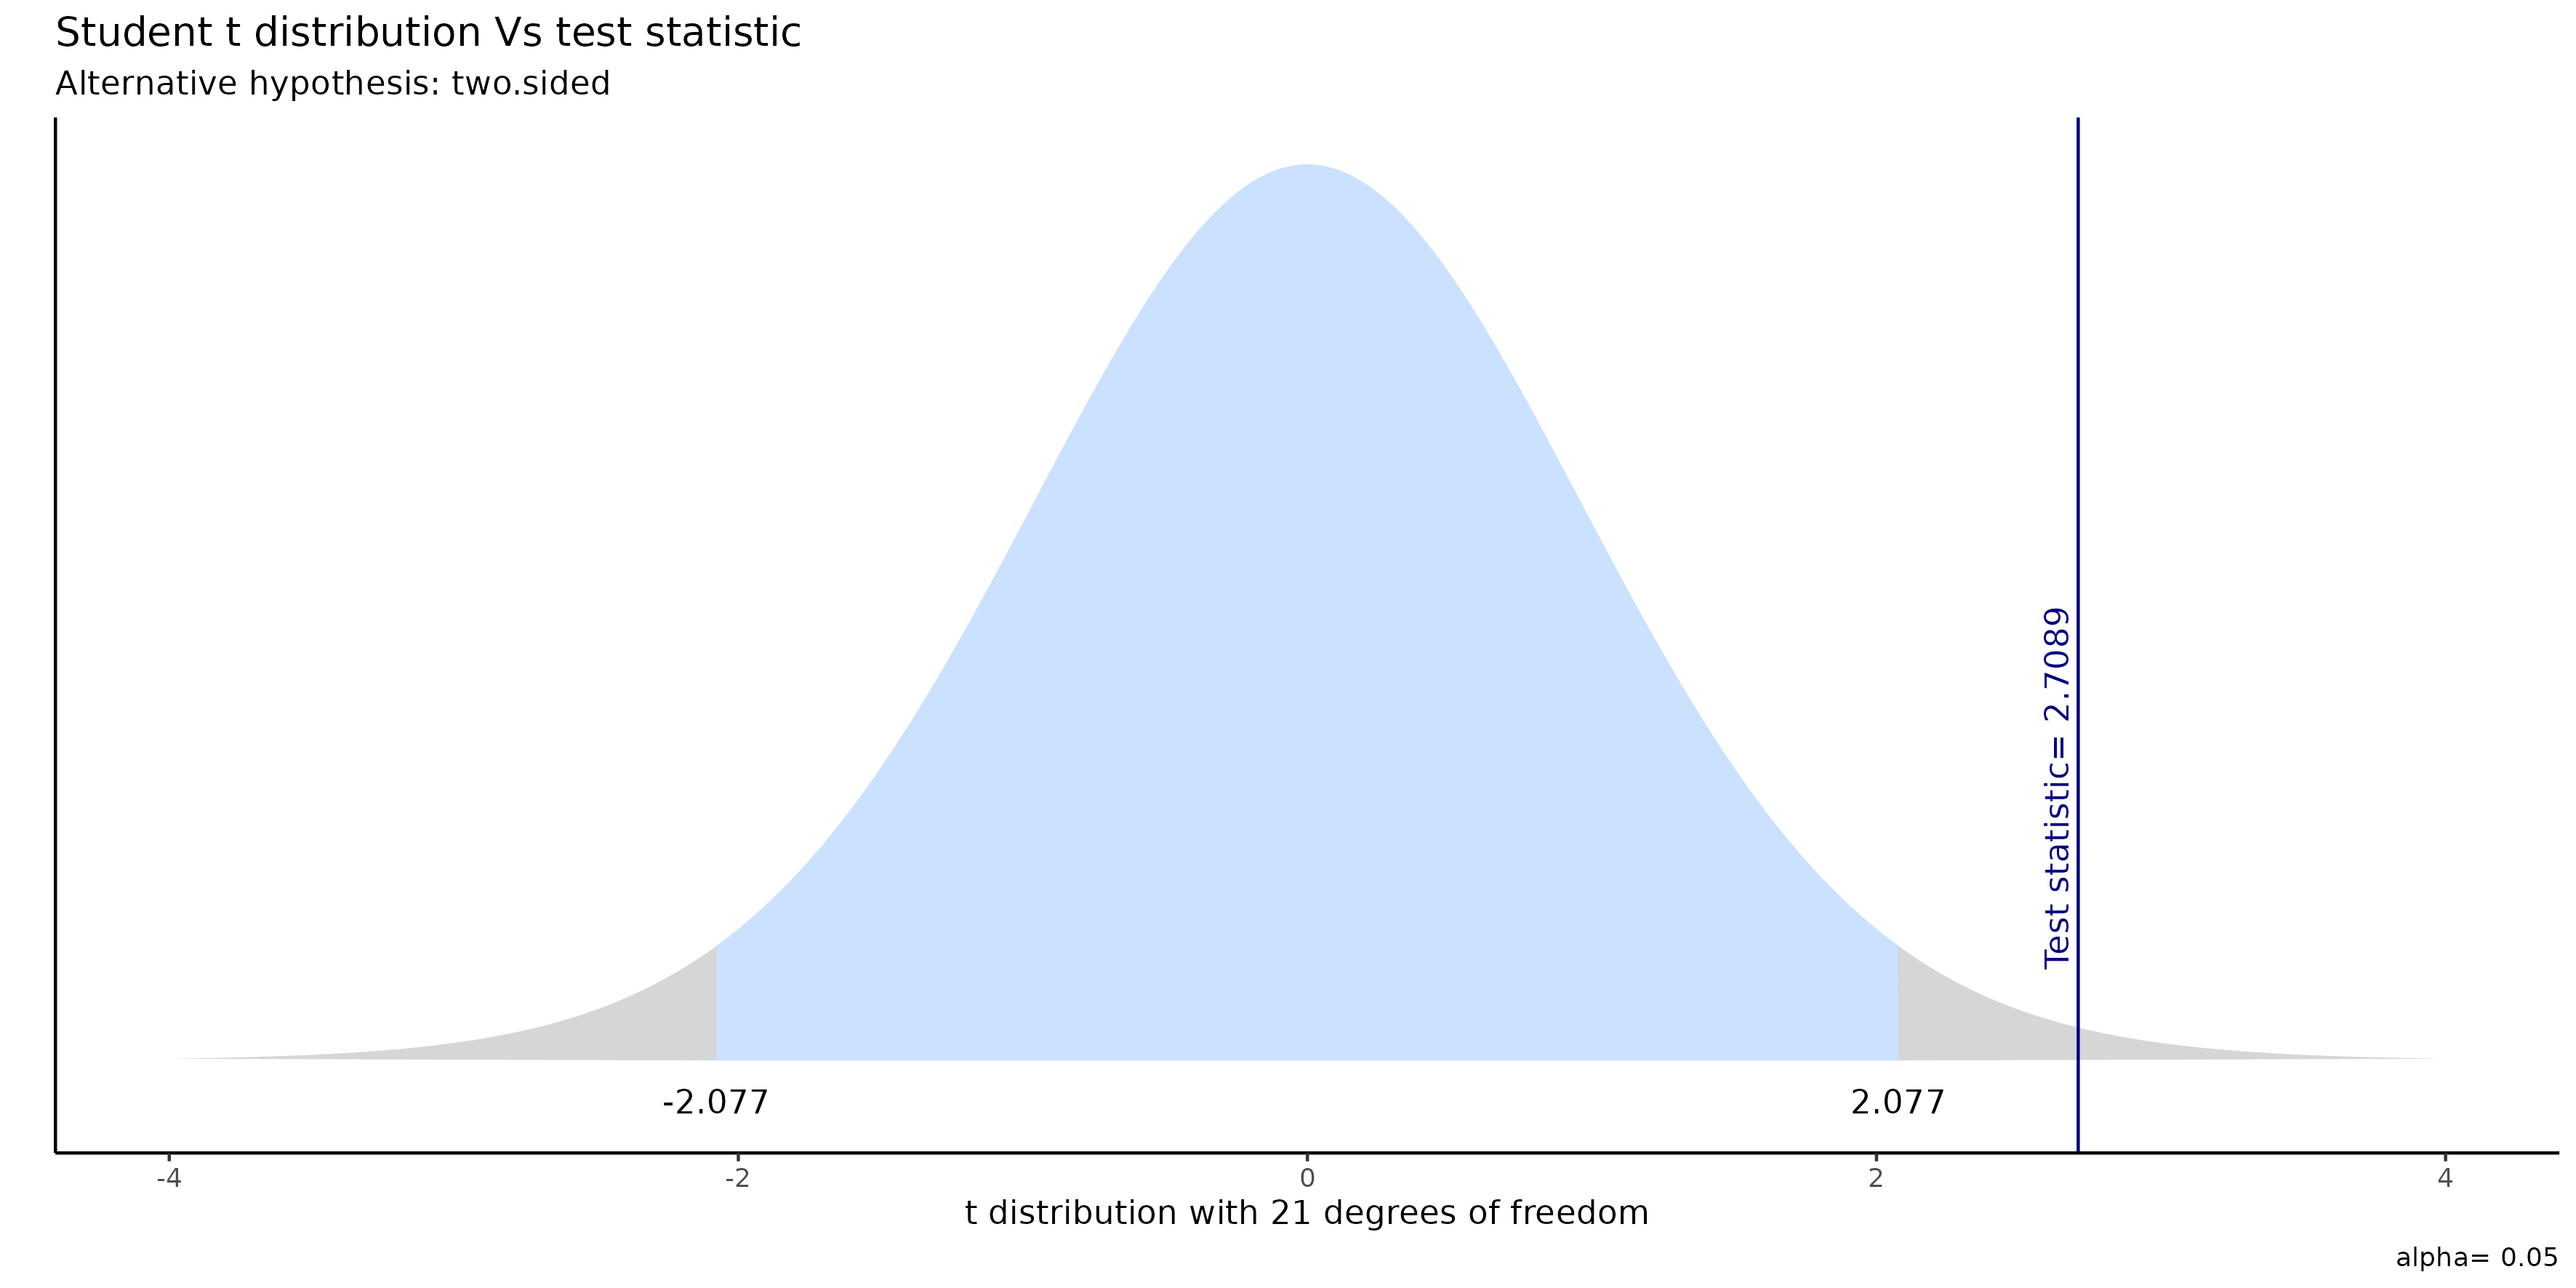
\includegraphics[width=\textwidth]{Img/cap2/pruebat_varianzasdiferentesFusarium_Shannon.png}
\caption{}
\end{figure}

\subsection{Prueba de Hipótesis sobre las varianzas de dos poblaciones pequeñas} 
Pon tu figura y describe tus resultados


Suponemos dos poblaciones independientes con distibuciones normales  

y queremos probar (tenemos como hipotesis nula)WilcoxonWilcoxon

$$H_{0} : \sigma_{1}^{2} = \sigma_{2}^{2}$$

respecto a la hipotesis alternativa

$$H_{a} : \sigma_{1}^{2} \neq \sigma_{2}^{2}$$

tomando como estadistico de prueba:

$$ F = \frac{S_{1}^{2}}{S_{2}^{2}}$$


\begin{figure}[!]
\centering
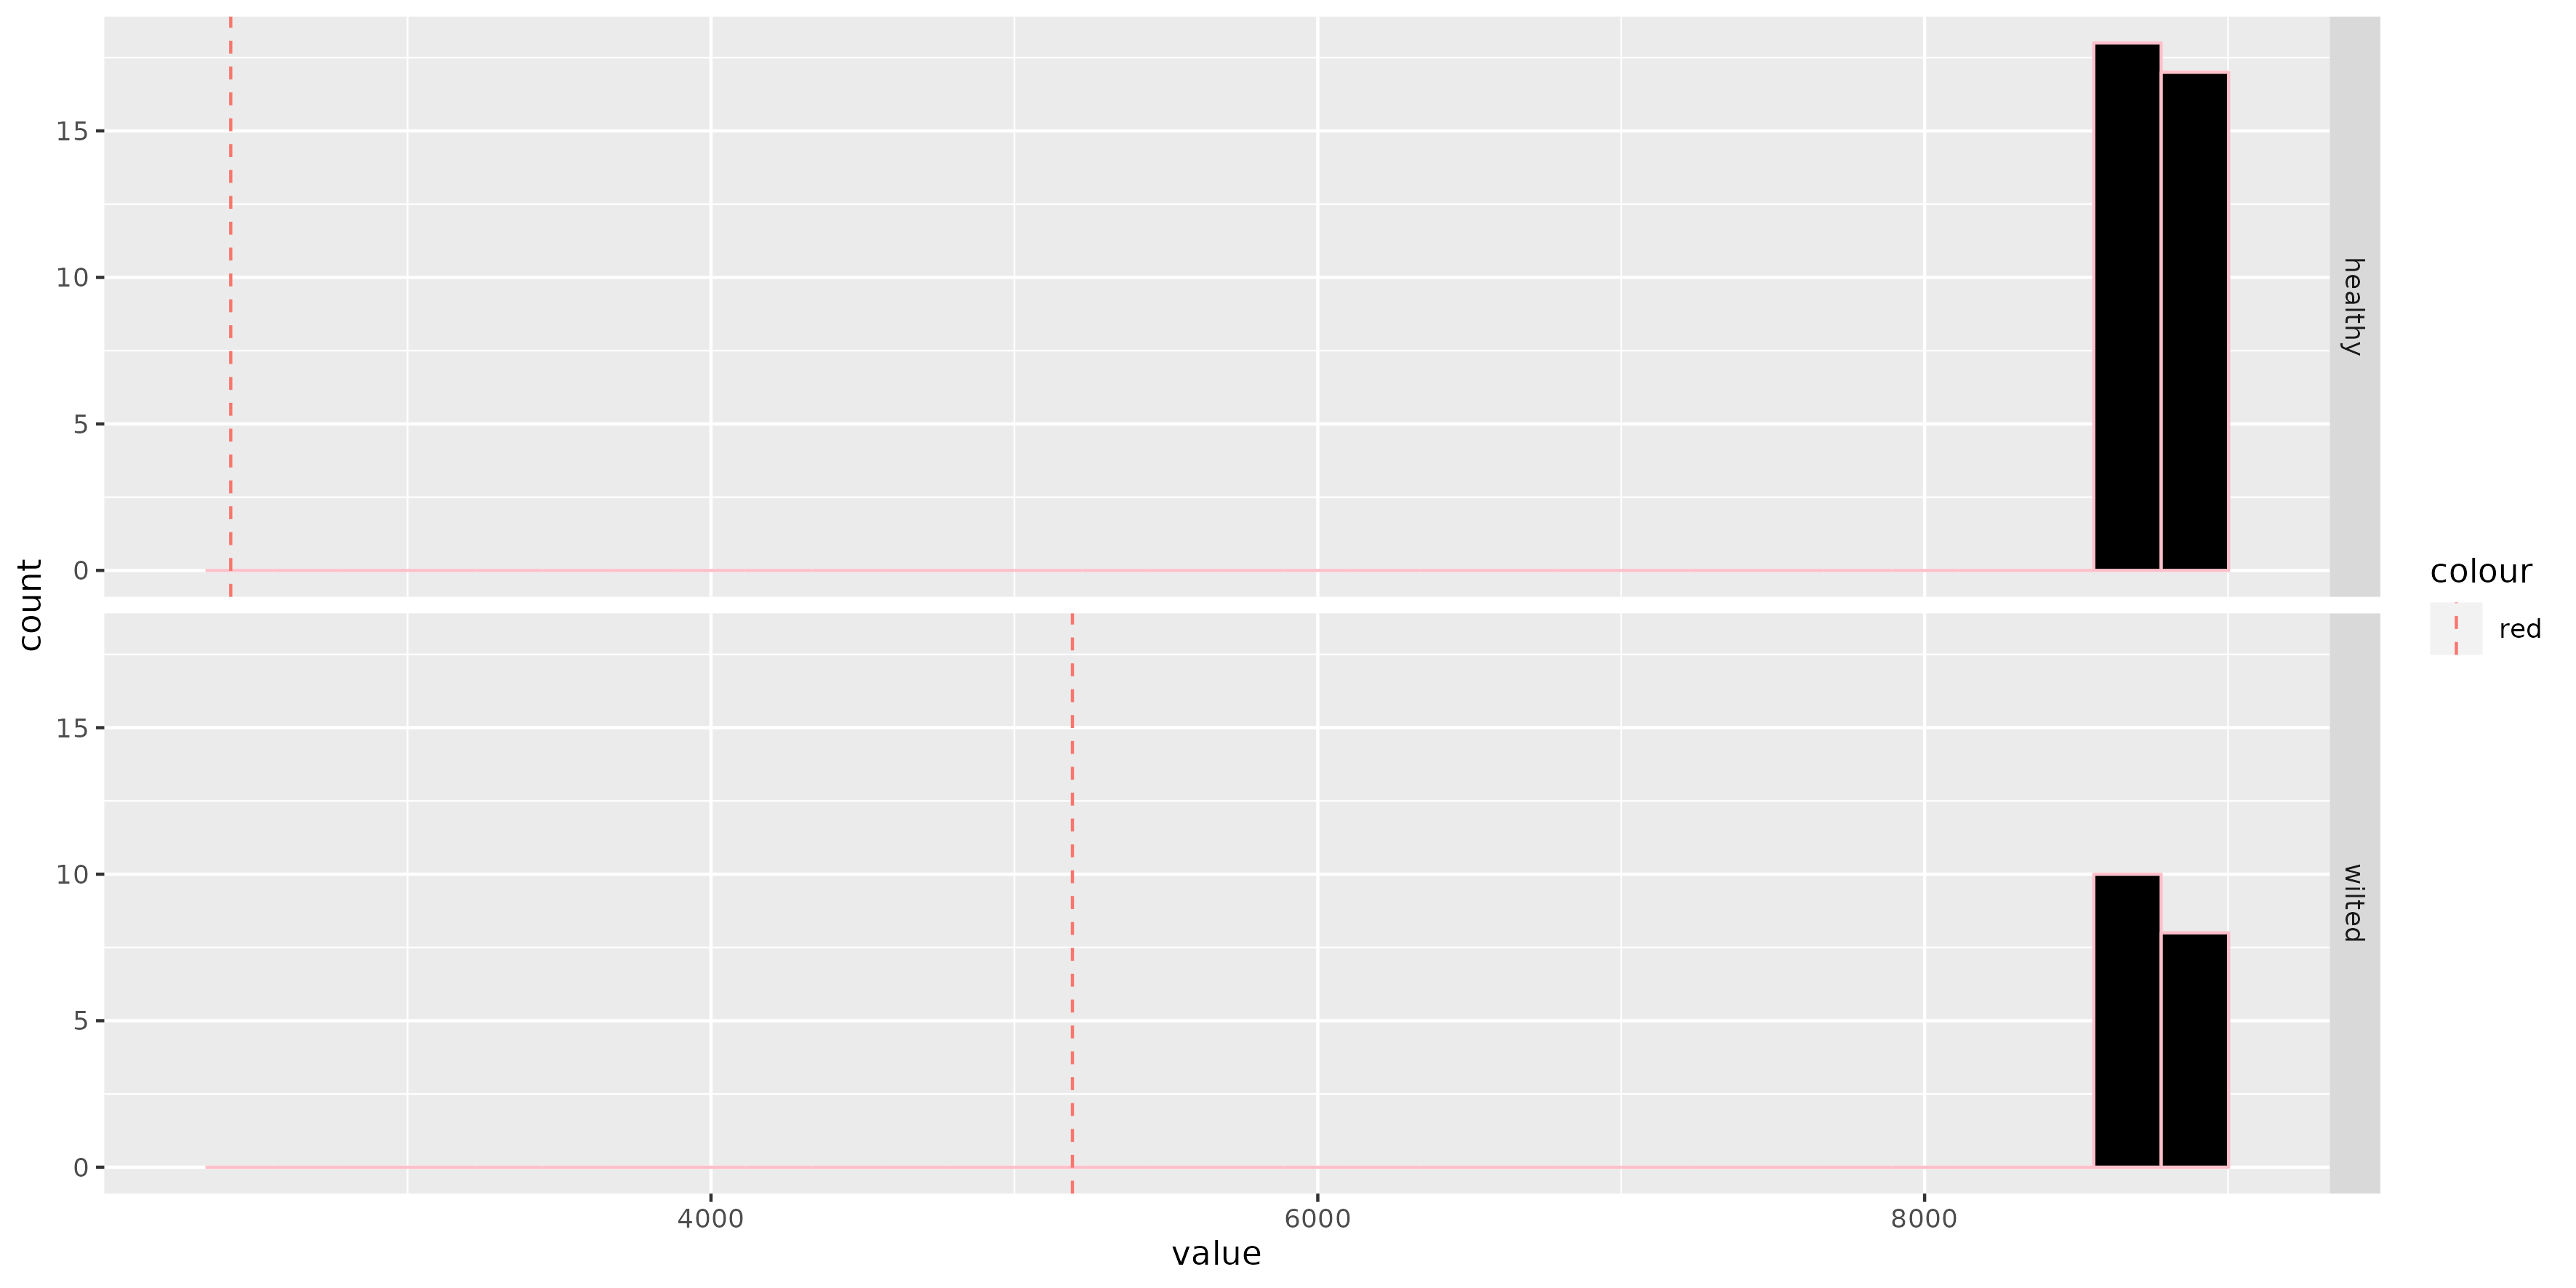
\includegraphics[width=\textwidth]{Img/cap2/varianzas_Chao1.png}
\caption{}
\end{figure}

\subsection{Prueba de los rangos con signos de Wilcolxon}

Esta es una prueba no parametrica para comparar el rango medio de dos muestras relacionadas y determinar si existen diferencias entre ellas. Se uso, ya que los datos no tienen una distribucion normal.

\begin{figure}[!]
\centering
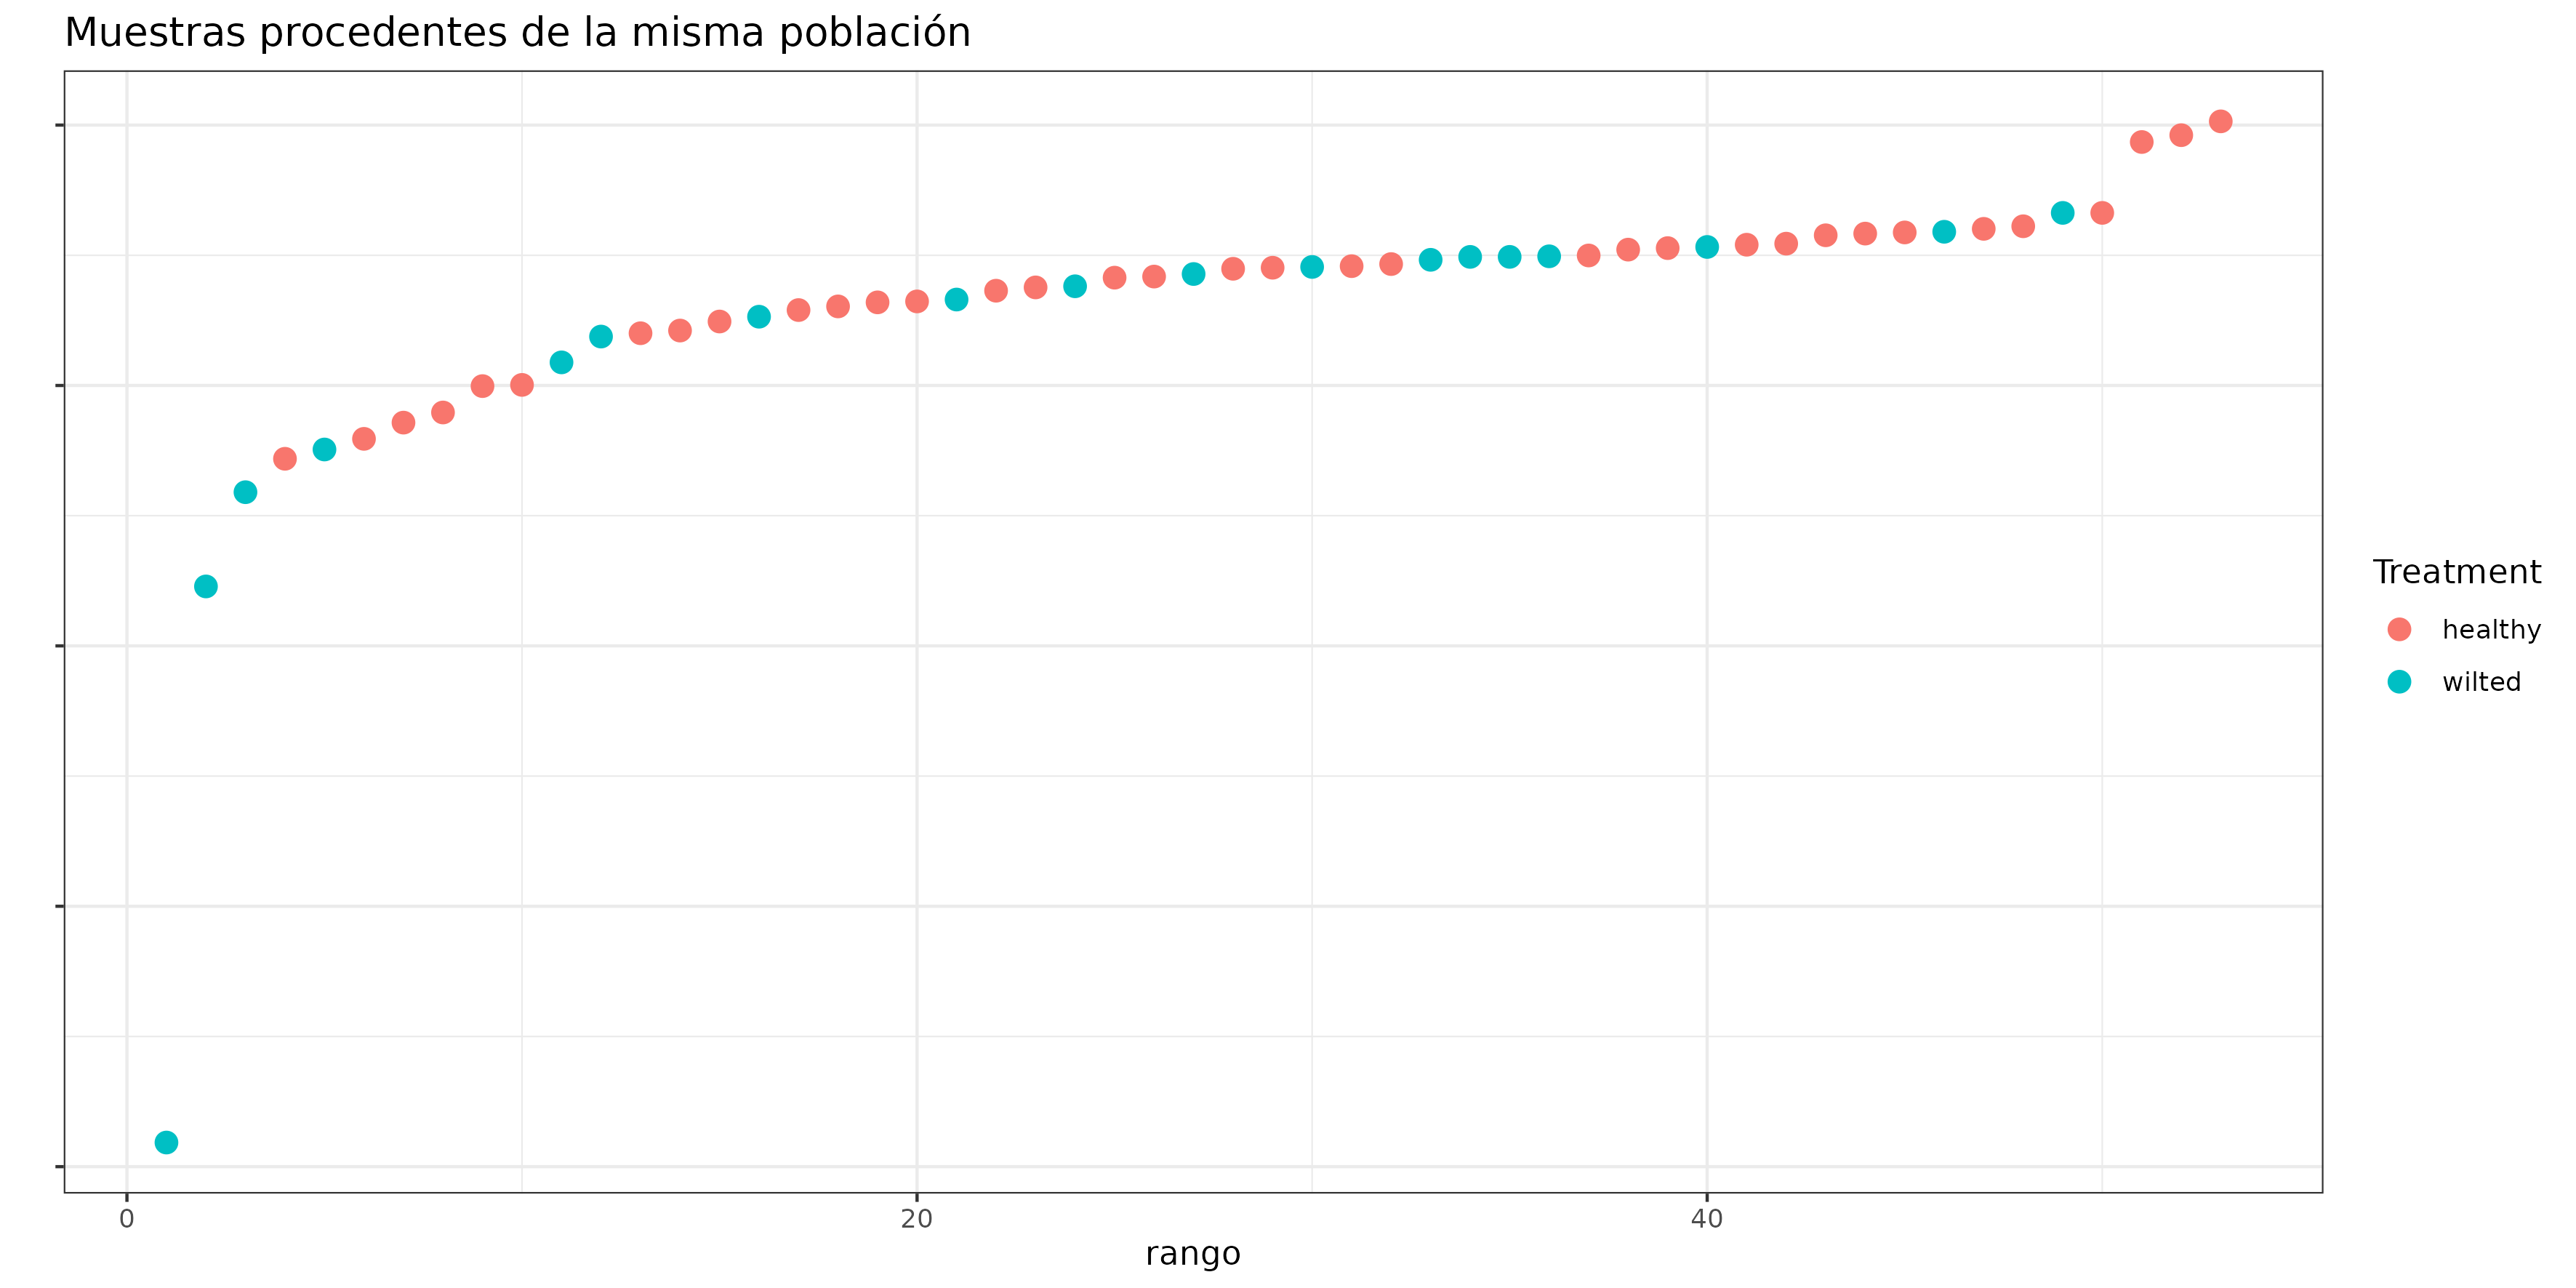
\includegraphics[width=\textwidth]{Img/cap2/Wilcoxon_Shannon.png}
\caption{Wilcoxon}
\end{figure}




Pon tu figura y describe tus resultados, y describe que es una prueba Wilcoxon


\subsection{Mann-Whitney}
La U de Mann-Whitney para comparar lasmedias dedos grupos independientes. 
Prueba no parametrica o libre de distribución, es el analogo no parametrico a la t de Student para lacomparacion de dos medias independientes; solo que esta no requiere parametros y se puede emplear sin ninguna condicion de aplicación.

\begin{figure}[!]
\centering
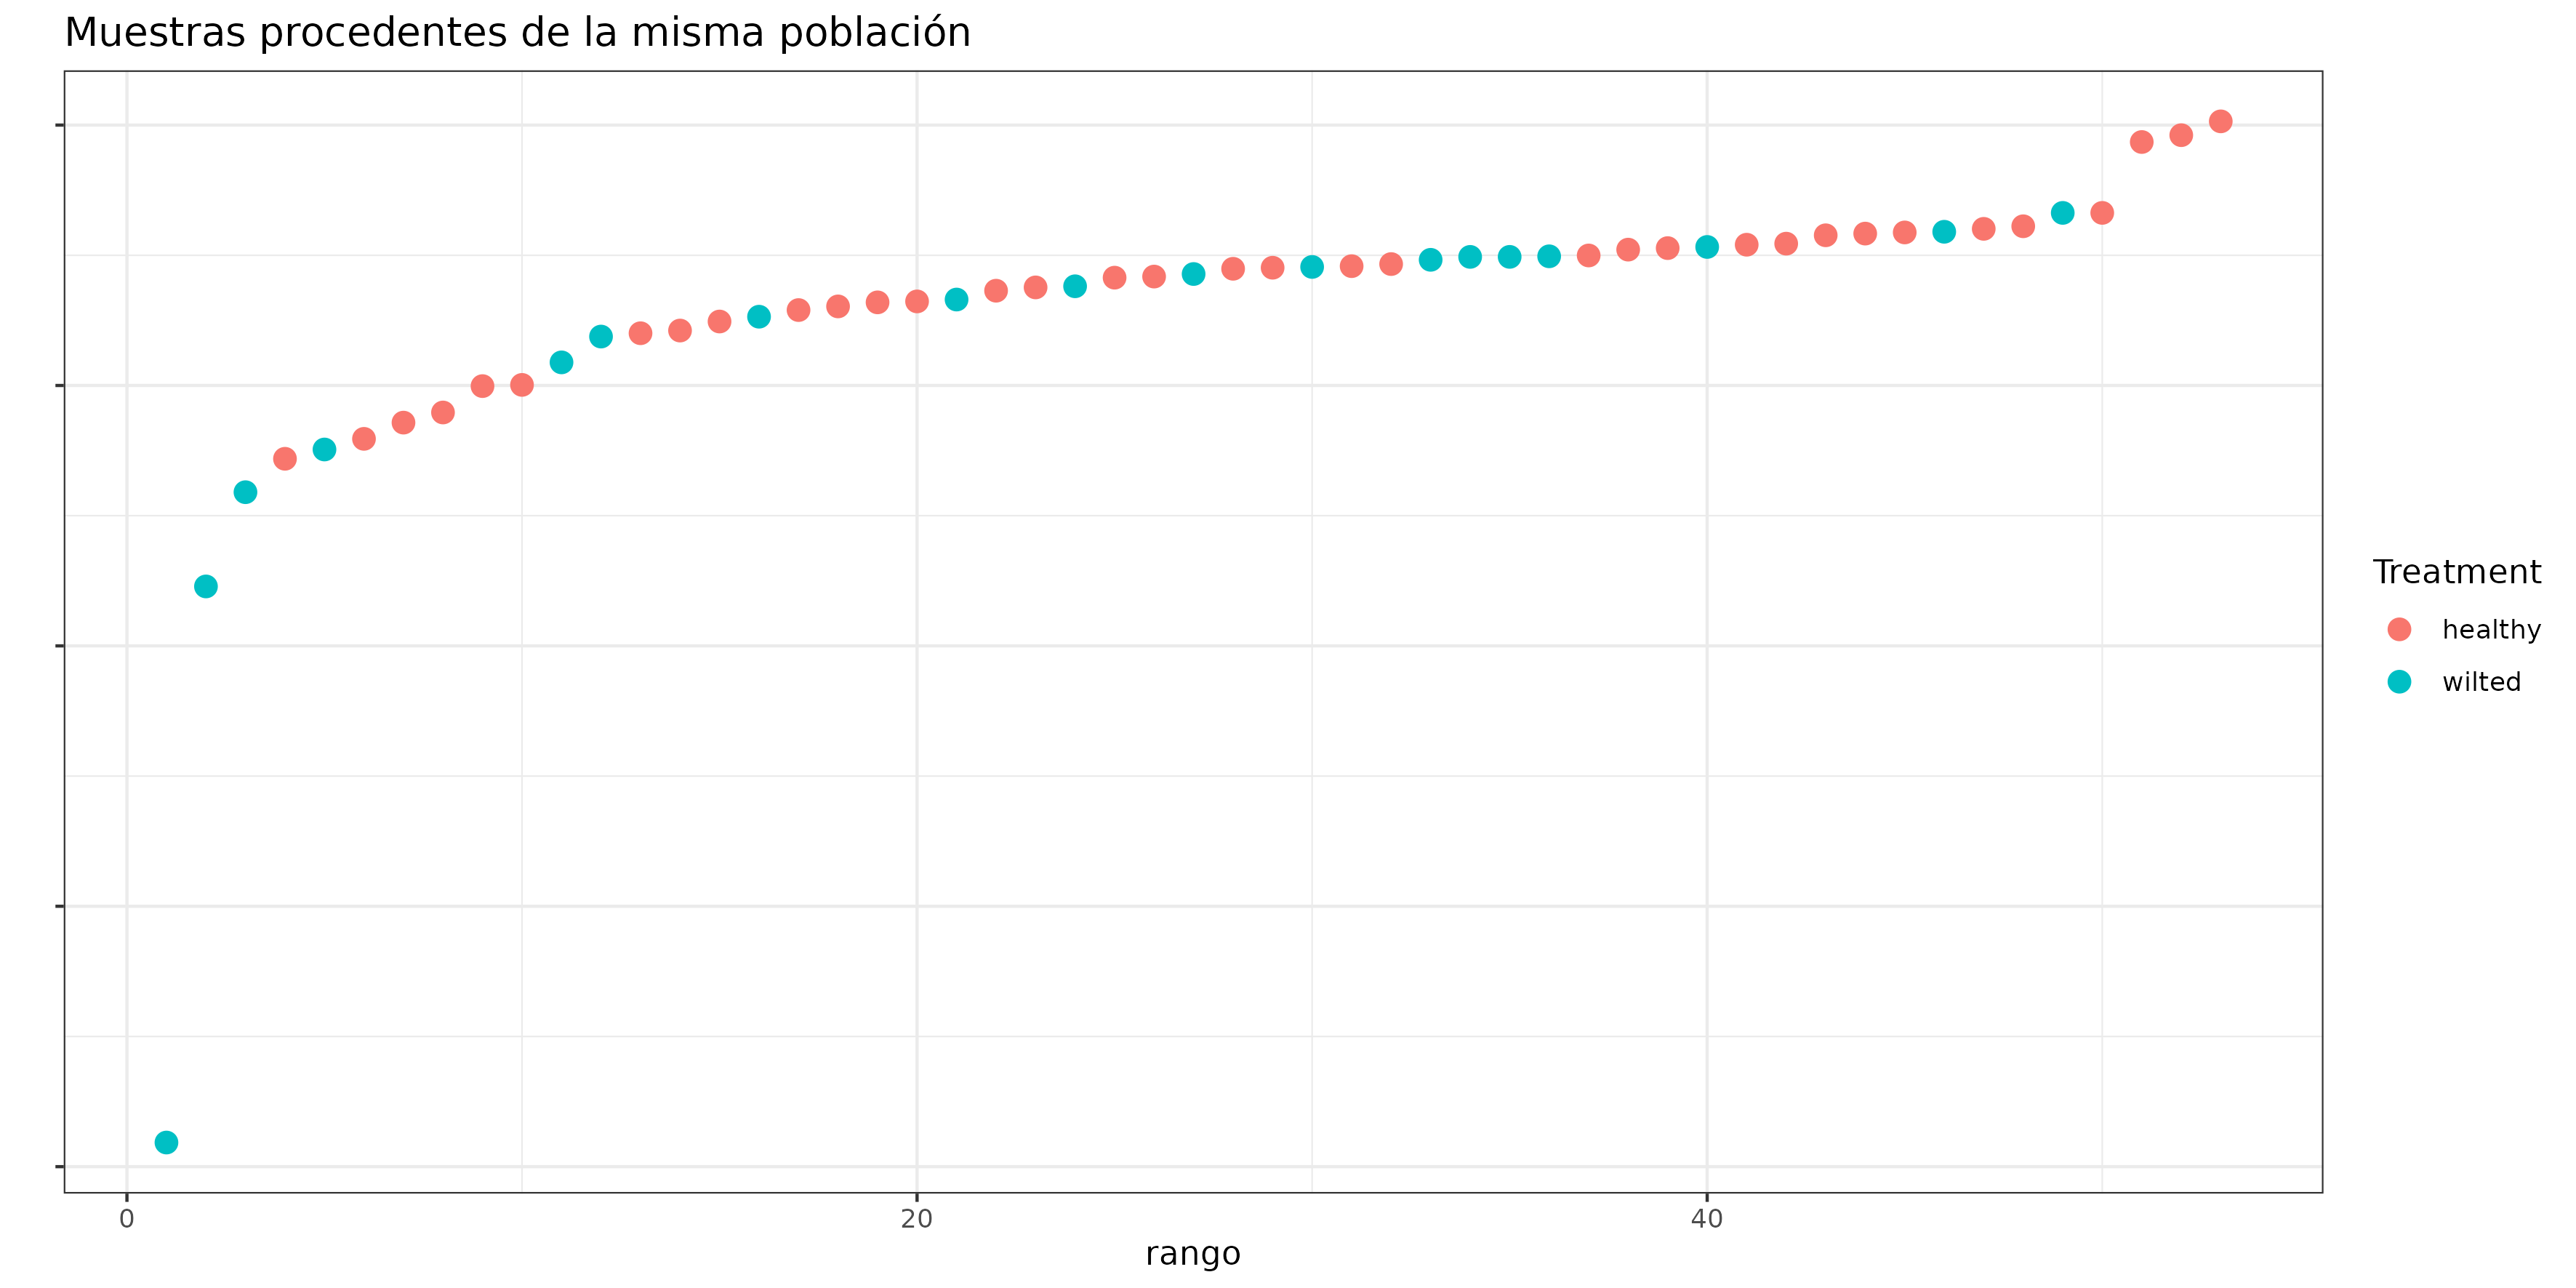
\includegraphics[width=\textwidth]{Img/cap2/Wilcoxon_Shannon.png}
\caption{Mann-Whitney}
\end{figure}



\section{Normalización}
\subsection{Normalización}

\begin{figure}[!]
\centering
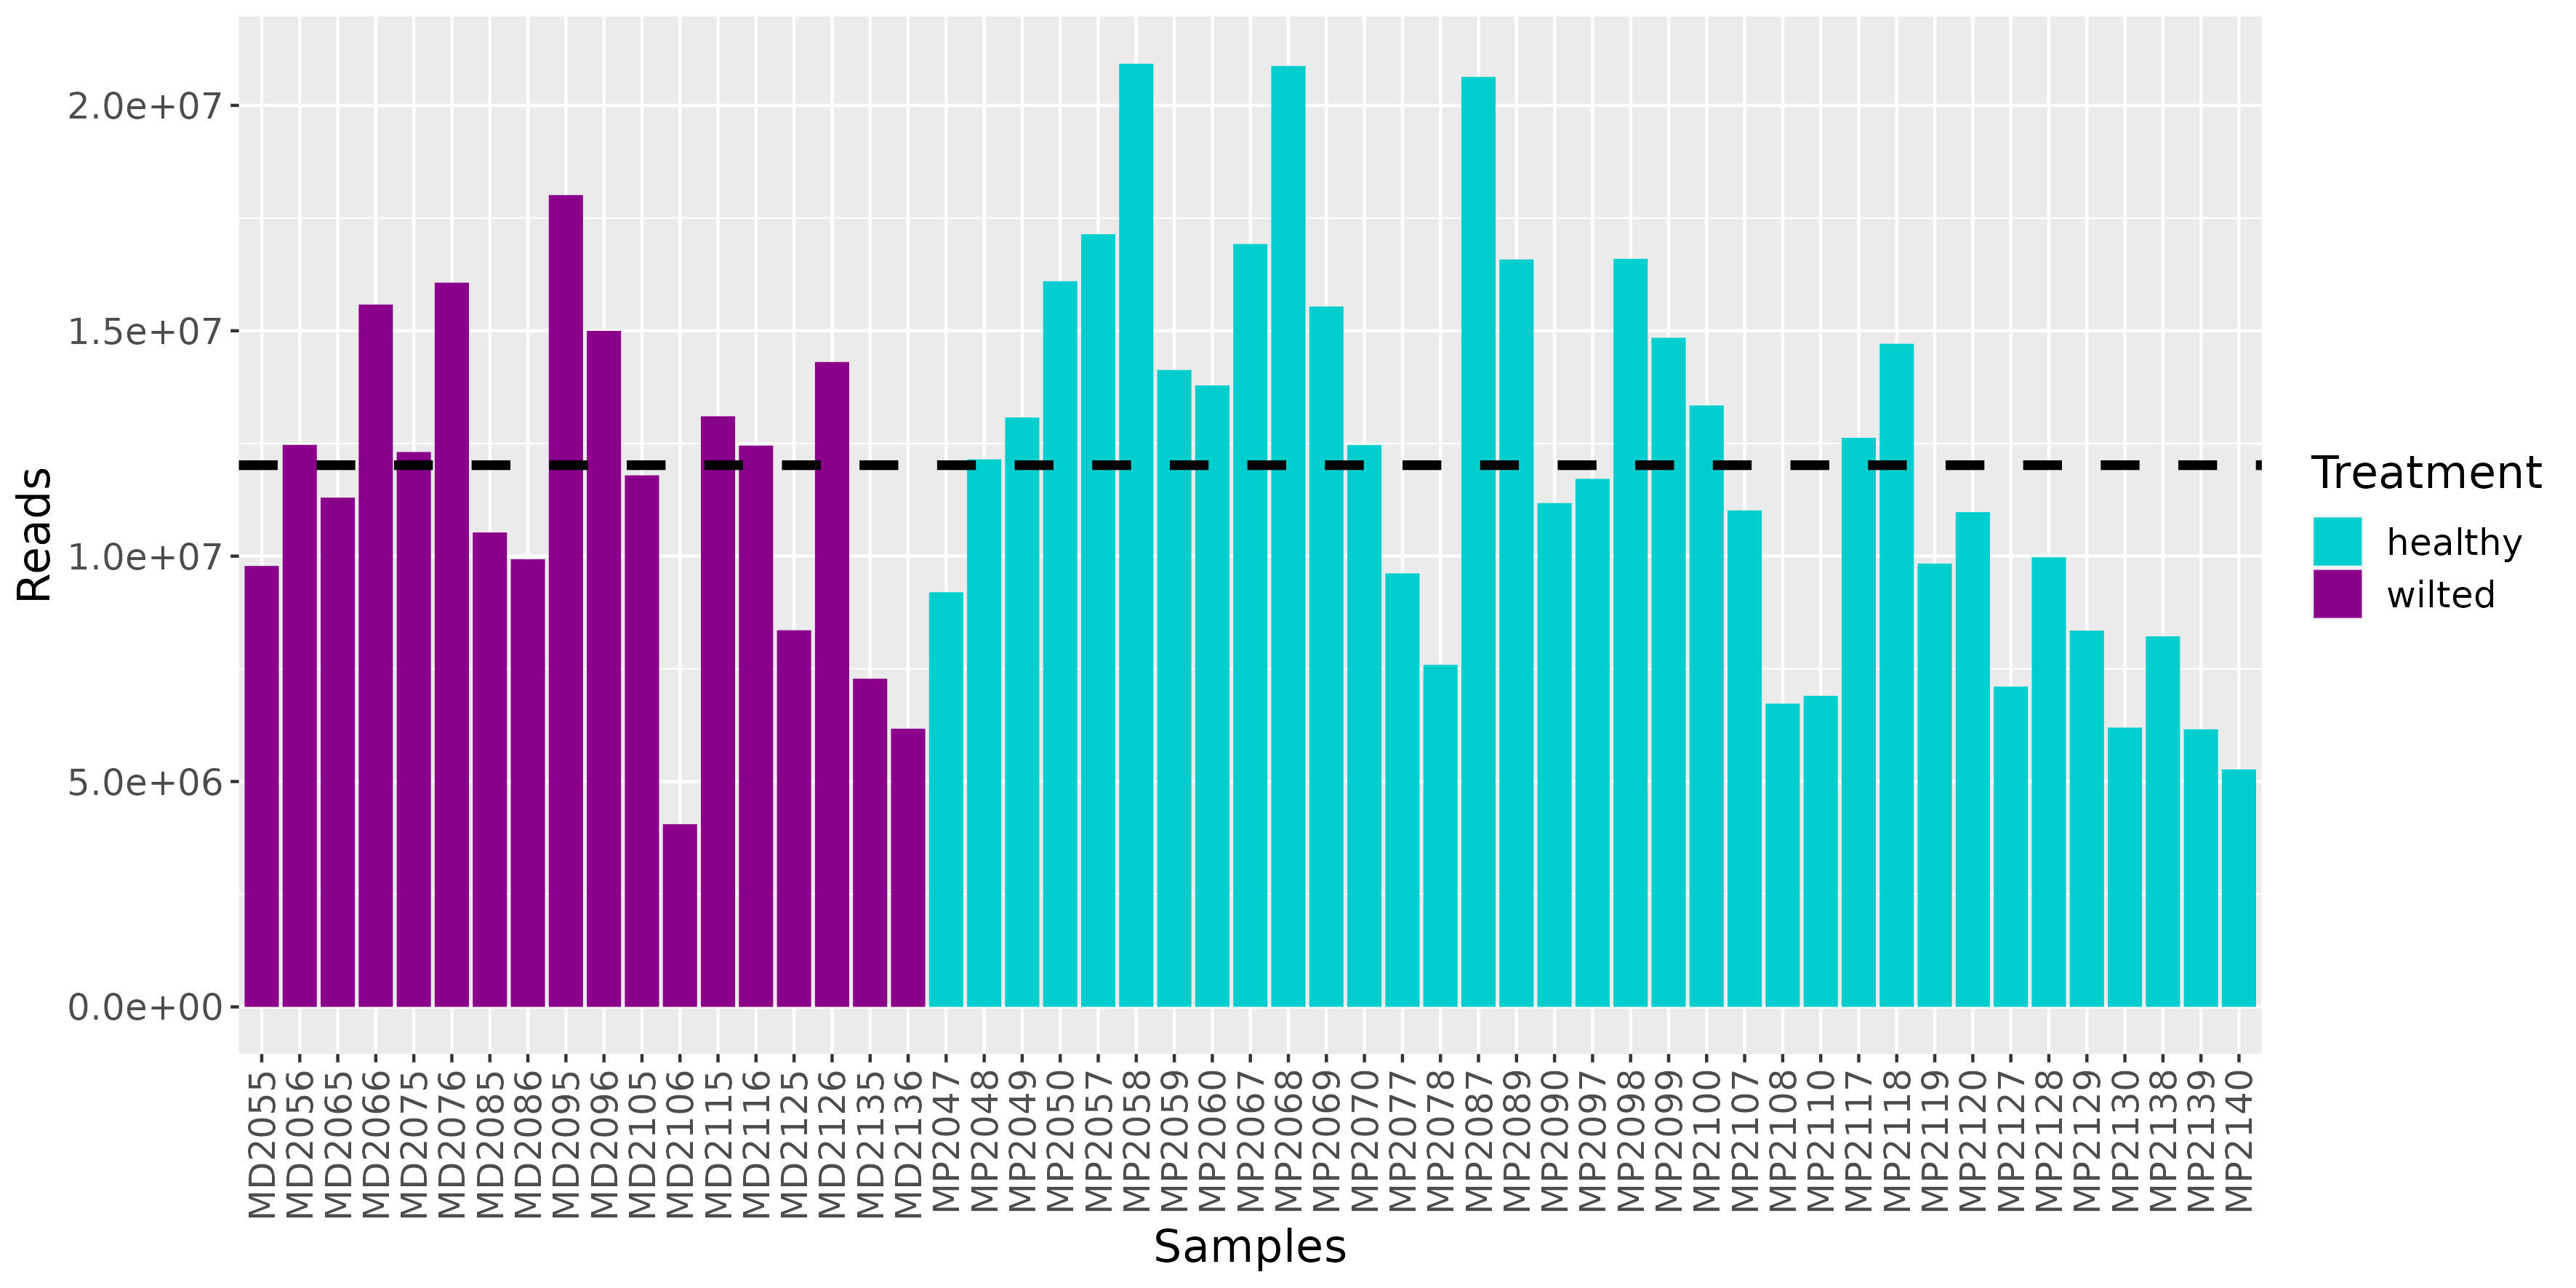
\includegraphics[width=\textwidth]{Img/cap2/Barras_Abundancia.png}
\caption{Barras de abundancia de los datos en crudo}
\end{figure}

La función edgeRnorm escala datos NGS normalizados utilizando la función de normalización provista en edgeR. Toma un objeto phyloseq y devuelve un objeto phyloseq cuya otu\_table se transforma.

\subsection{Rarefacción}
La rarefacción es una tecnica de normalización usada en el preprocesamiento de datos, para equilibrar el tamaño de las muestras en un conjunto de datos. Esta implica un submuestreo aleatorio de secuencias

Rarefy 

Se eliminaron 670 OTUs



\begin{figure}[!]
\centering
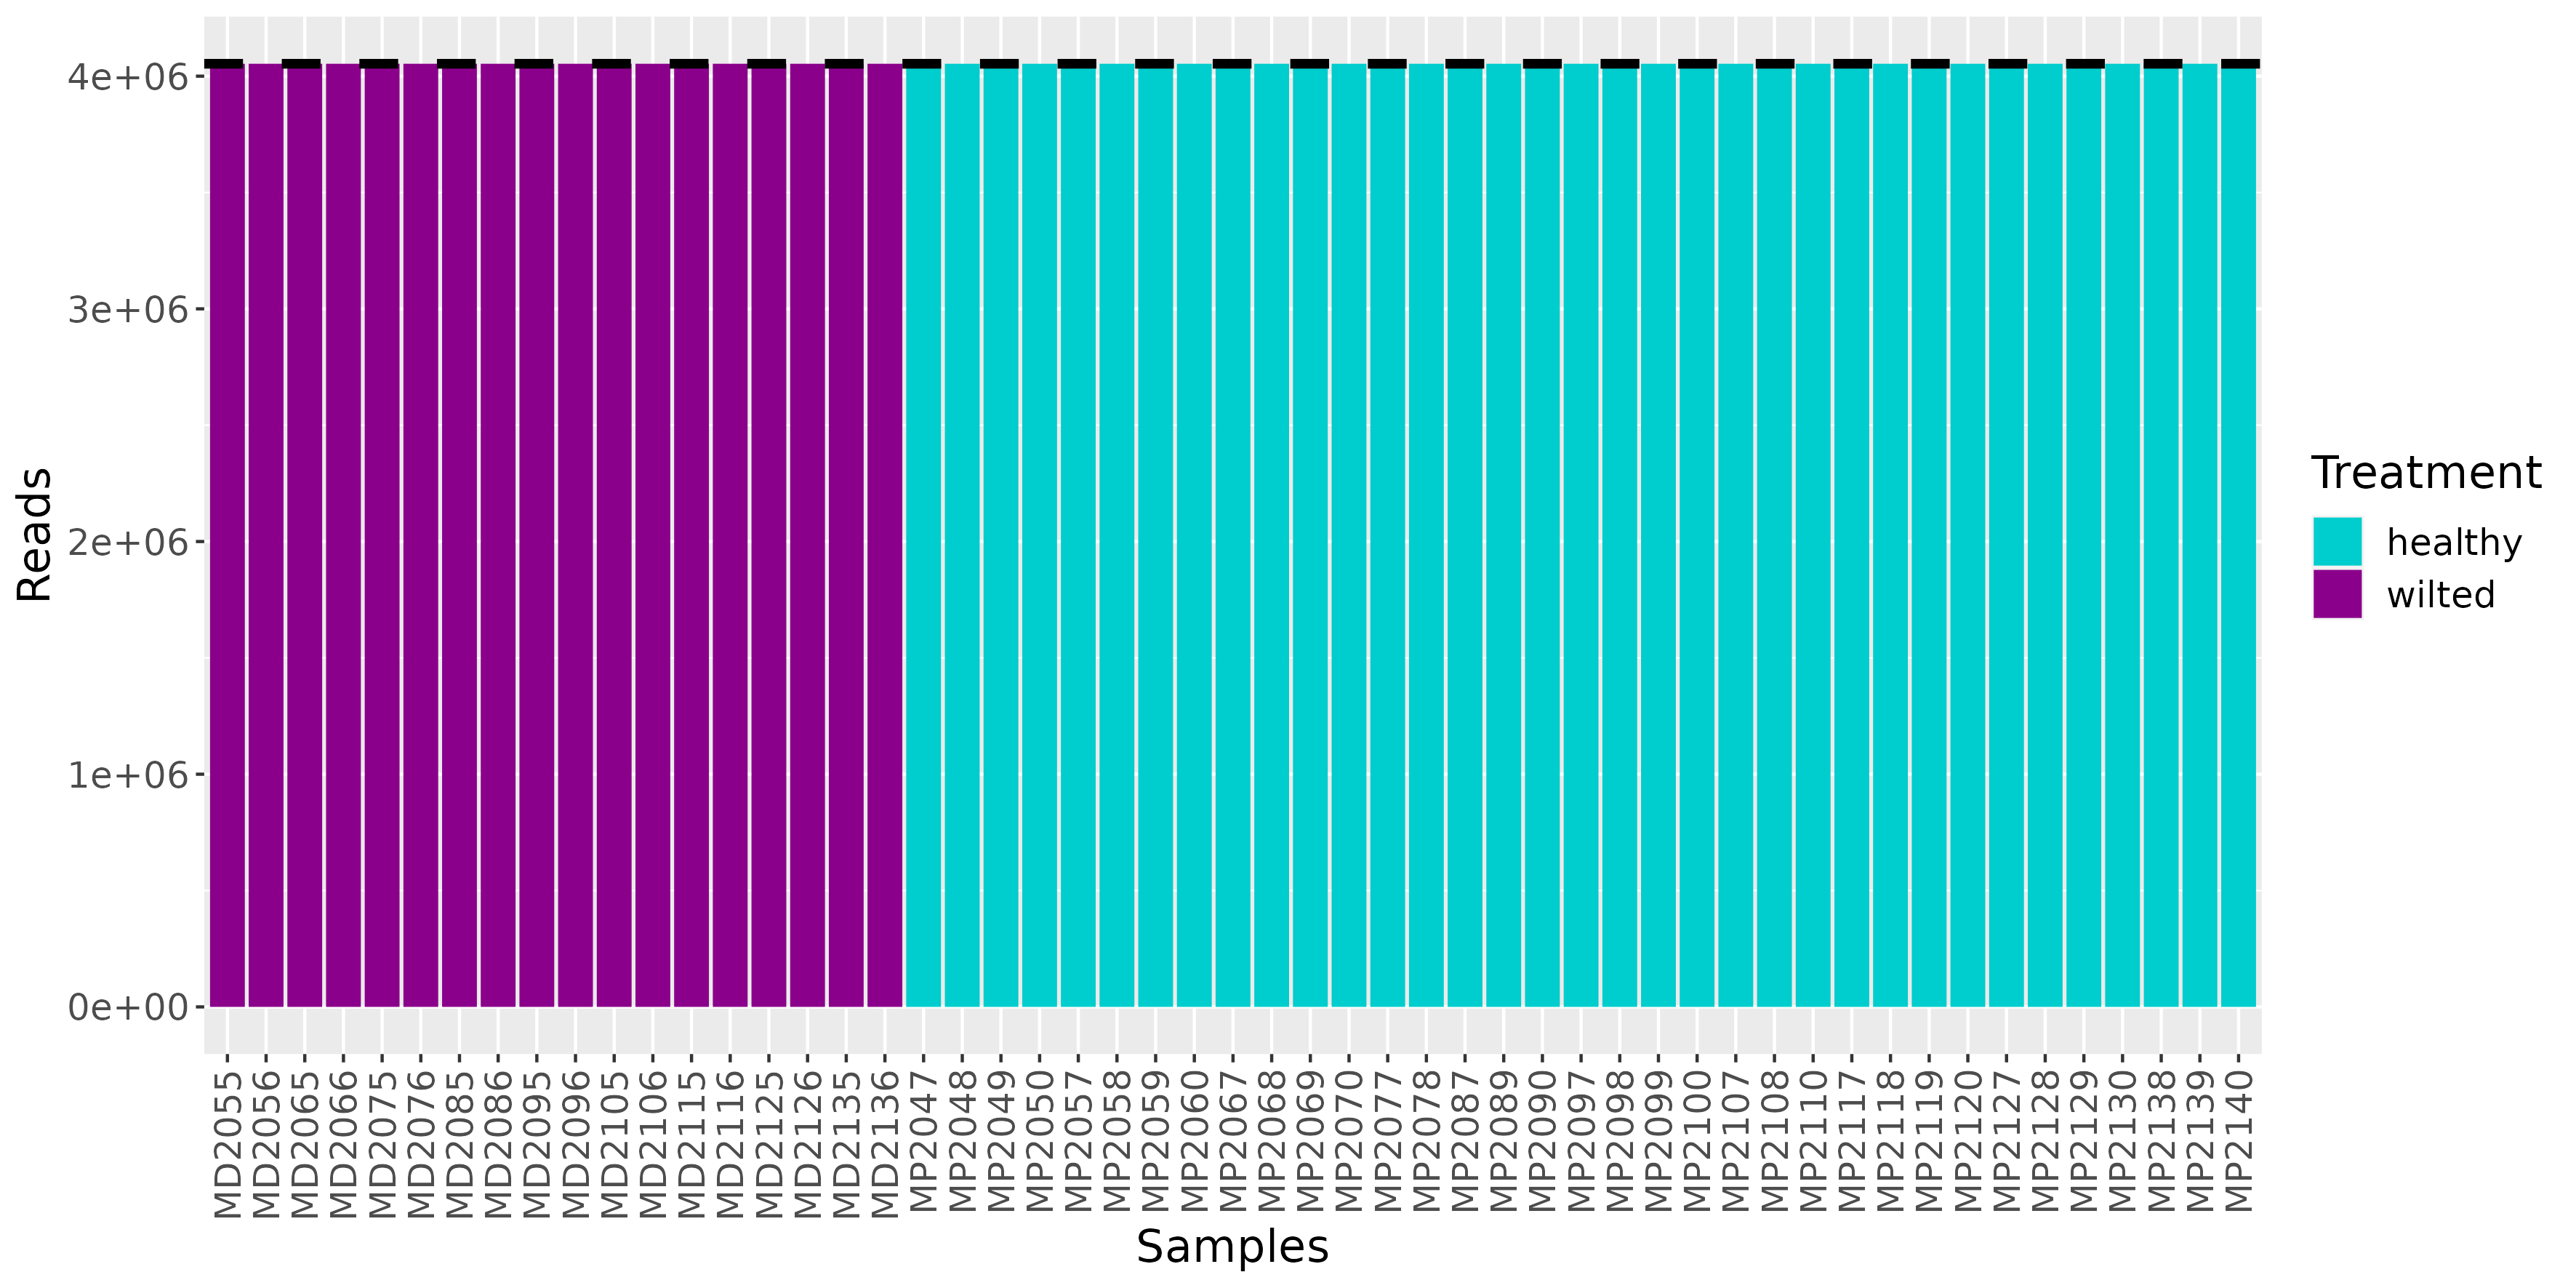
\includegraphics[width=\textwidth]{Img/cap2/Rarefaccion.png}
\caption{Barras de abundancia, luego de la rarefacción}
\end{figure}

\begin{figure}[!]
\centering
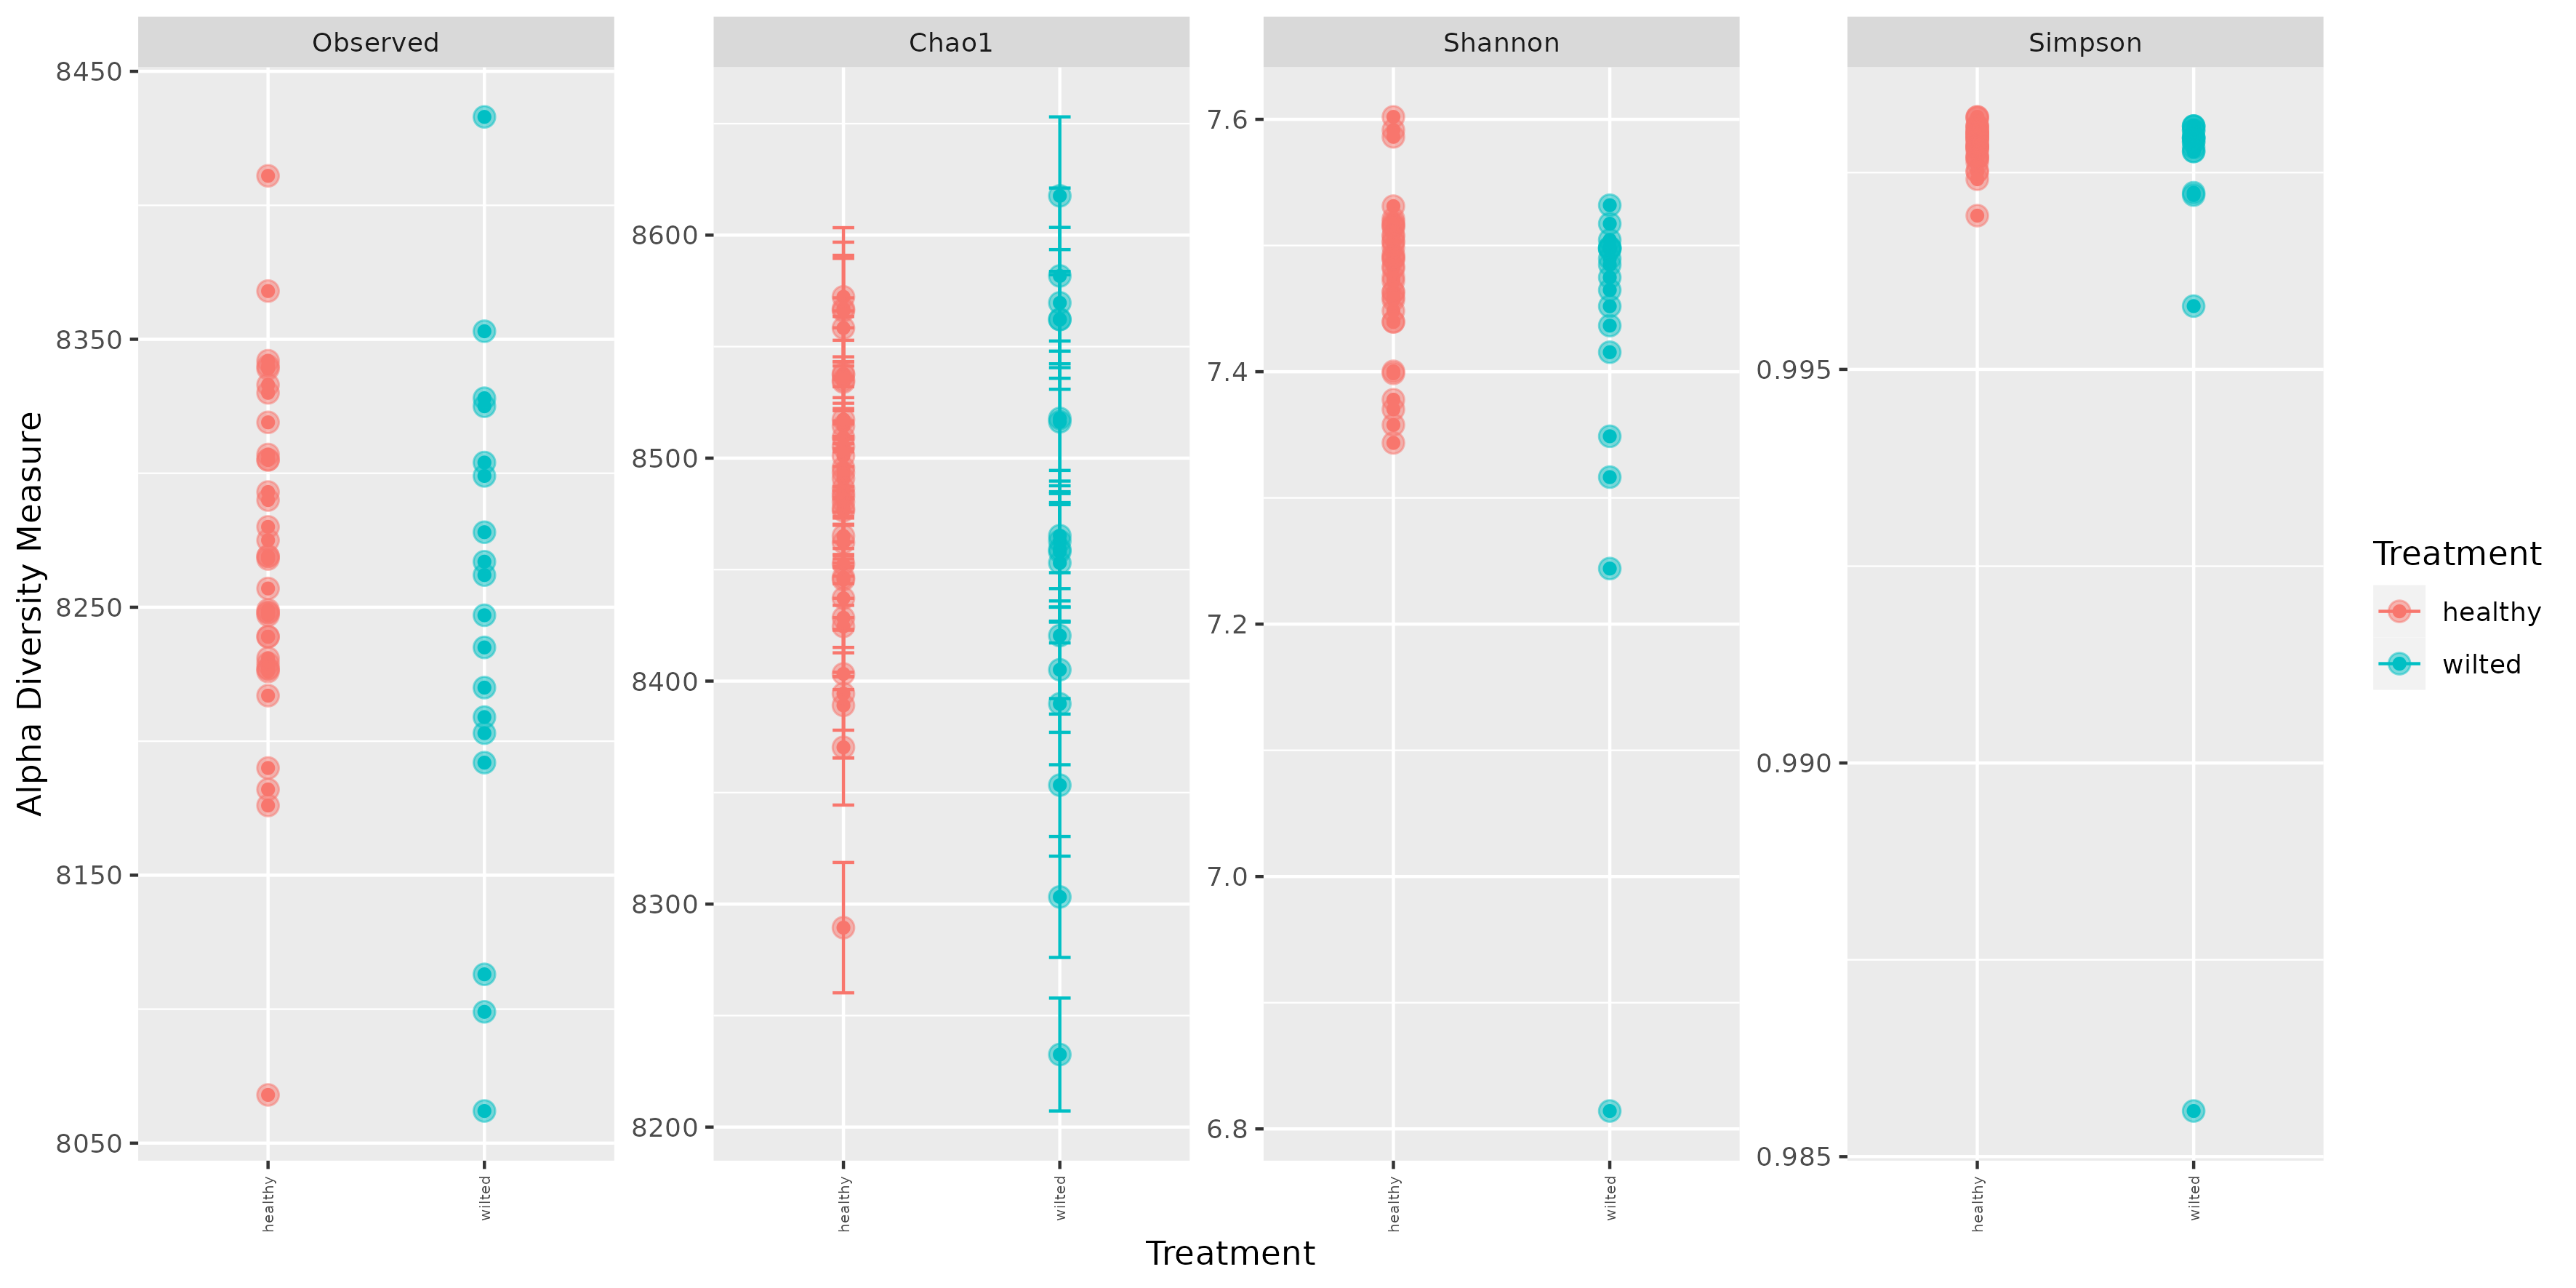
\includegraphics[width=\textwidth]{Img/cap2/Rarefaccion_diversidadAlfa.png}
\caption{Diversidad alfa luego de la rarefacción}
\end{figure}

\begin{figure}[!]
\centering
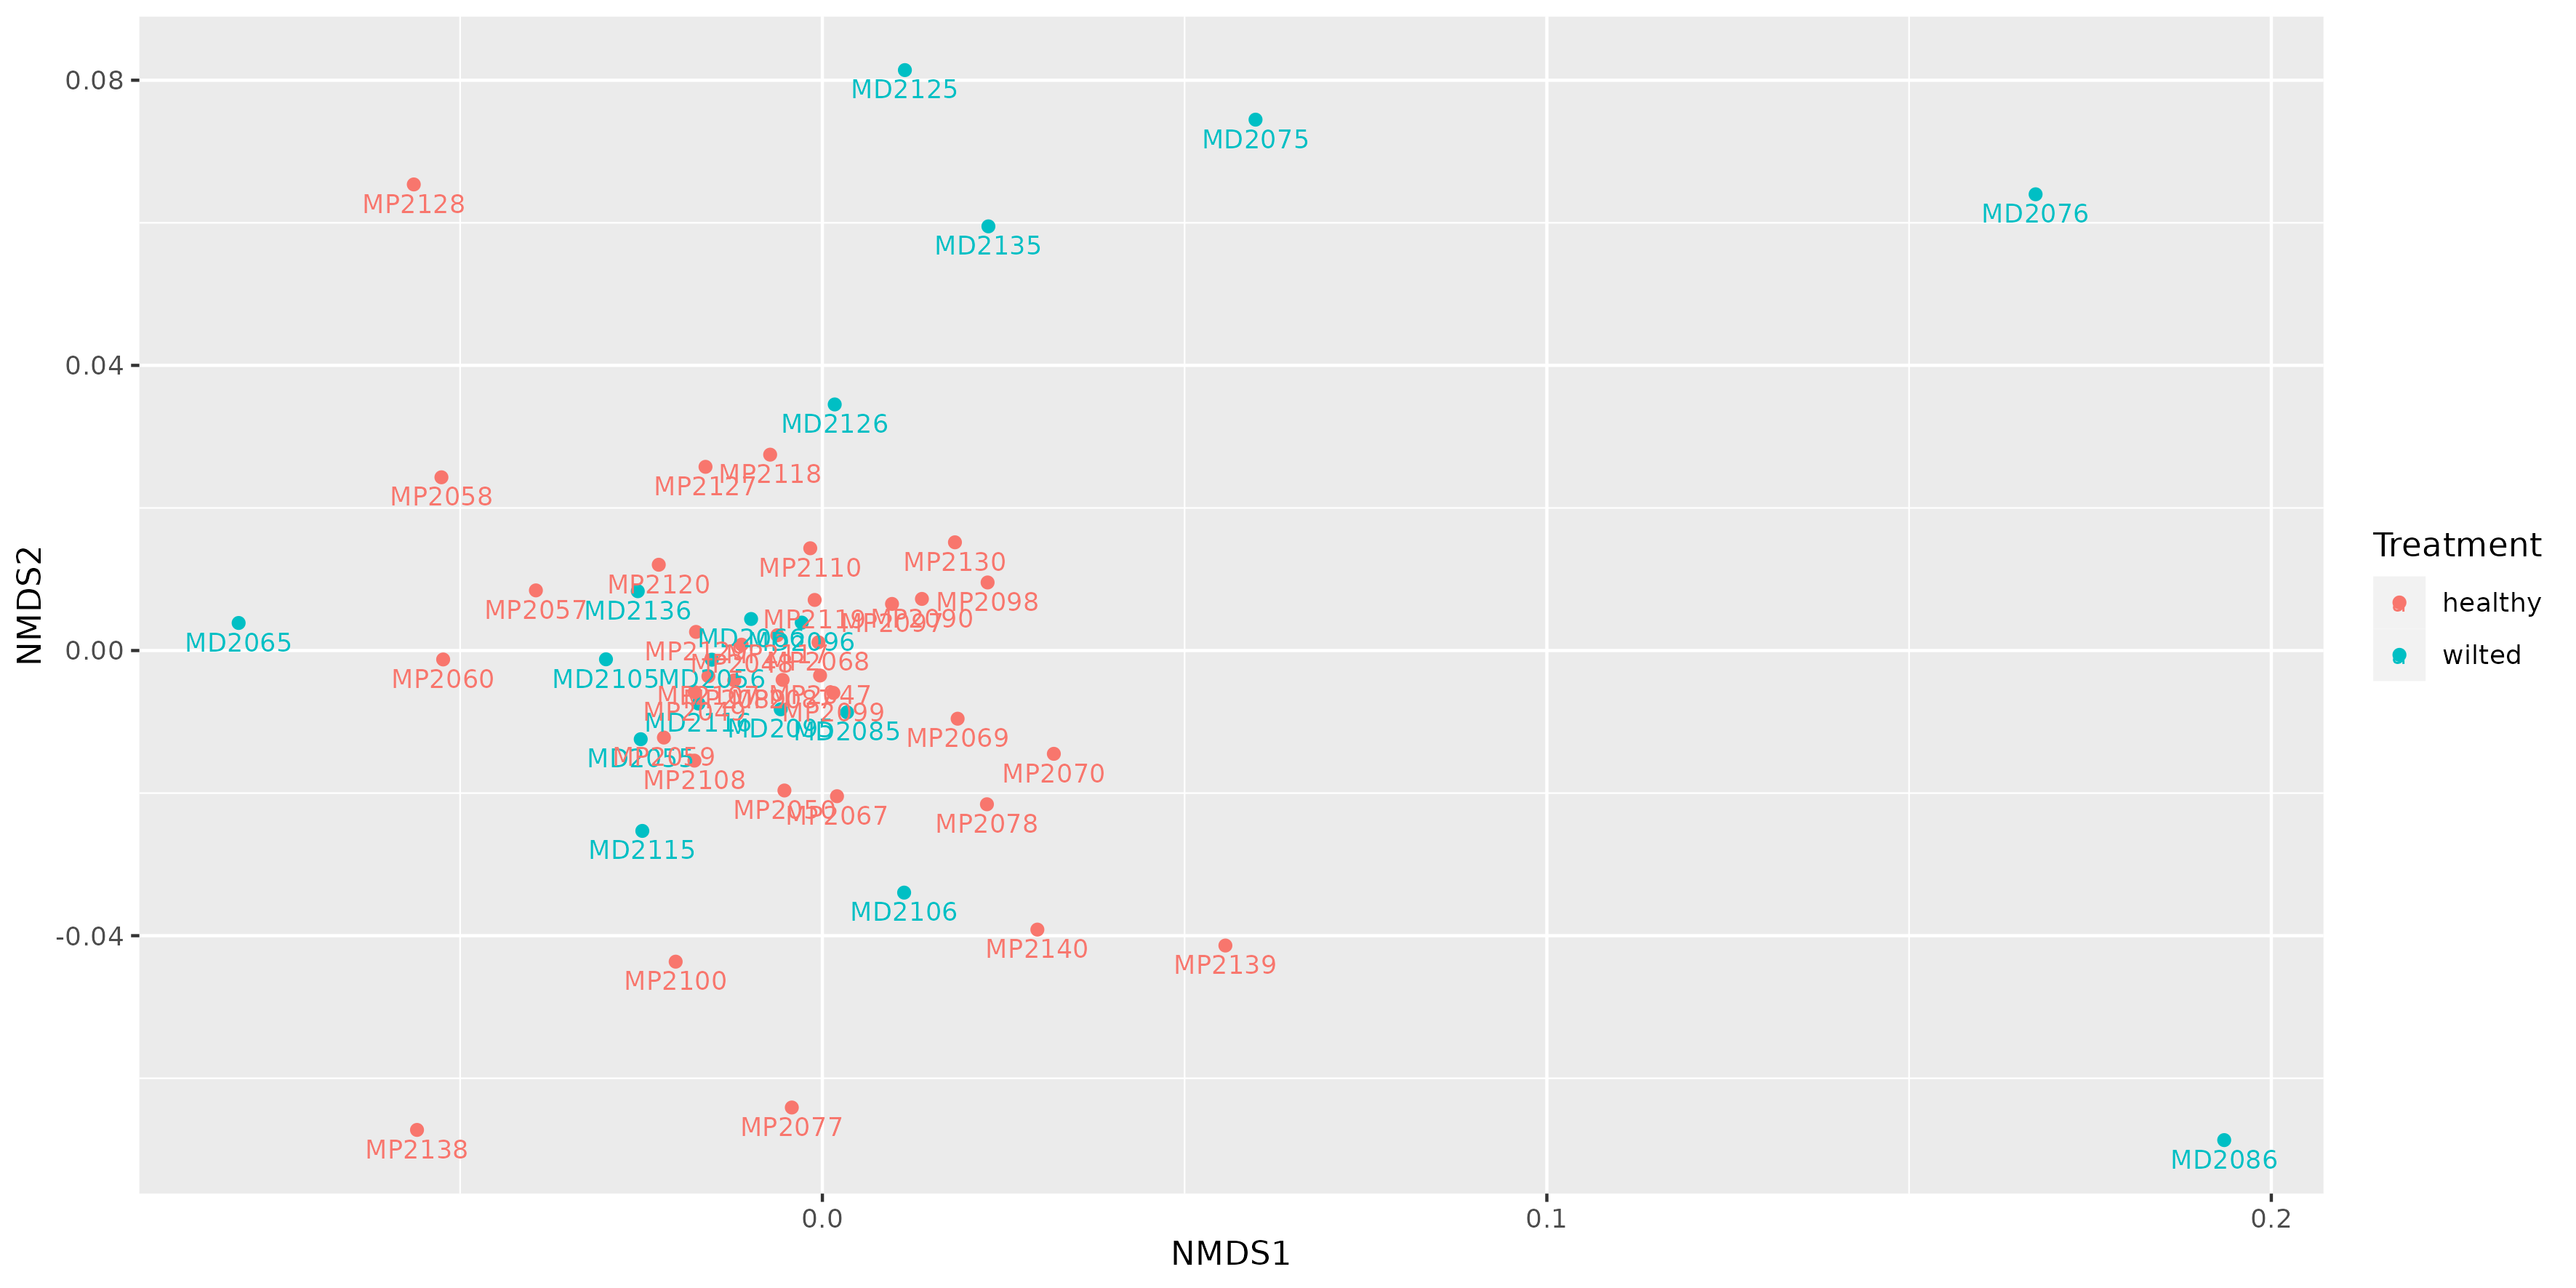
\includegraphics[width=\textwidth]{Img/cap2/Rarefaccion_diversidadBeta.png}
\caption{Diversidad beta luego de la rarefacción}
\end{figure}

\section{Rarefacción}
La rarefacción se usa como una medida de saturacion de muestras, es decir, 




\section{Redes}





Para poder visualizar las redes de nuestros datos, podemos hacer un data.frame uniendo toda la informacion
del objeto phyloseq.\\

\begin{lstlisting}
    df <- psmelt(fresa_kraken_fil)
\end{lstlisting}

Hay dos funciones en el paquete phyloseq para trazar la red del microbioma usando “ggplot2”: plot\_network() y plot\_net().
Se crea un grafo basado en “igraph”, basado en el método de distancia por defecto, Jaccard y una distancia
máxima entre nodos conectados de 0,8. El “Treatment” se utiliza para los mapeos de color y forma para
visualizar la estructura de las muestras.

Hacemos un grafo a partir de el objeto phyloseq

\begin{lstlisting}
    ig <- make_network(fresa_kraken_fil, max.dist=0.8)
\end{lstlisting}

Y luego lo graficamos.

\begin{lstlisting}
    plot_network(ig, fresa_kraken_fil, color="Treatment", shape="Treatment")
\end{lstlisting}

\textbf{INSERTAR AQUI IMAGEN DEL GRAFO}

En este grafo podemos ver la complejidad de los datos y las conexiones entre nuestras muestras.\\

En comparacion con la función plot\_network(), la nueva función plot\_net() no requiere una llamada separada a la función make\_network(), o un objeto igraph separado. Los siguientes códigos crean una red basada en una distancia máxima entre los nodos conectados de 0,5.

\begin{lstlisting}
    plot_net(fresa_kraken_fil, maxdist = 0.5, color = "Treatment", shape="Treatment
\end{lstlisting}

\textbf{INSERTAR AQUI IMAGEN DEL GRAFO}

En conclusion para esta observación general de los datos, no es posible ver una separacion entre muestras
sanas y enfermas claramente con la diversidad beta,y con los graficos de barras y redes, no es posible
identificar datos especiales.




\textbf{PONER GRAFOS Y DATOS DE REDES HECHAS CON FONTY}

Luego de una breve visualizacion de redes simples, tenemos dos opciones para utilizar ls redes de coocurrencia

El analisis de co-ocurrencia utiliza la matriz de interacciones
Redes de co-ocurrencia - El total de nodos de la red es el numero de OTU's en una tabla; se quiere ver las relaciones entre nodos. LAs aristas representan co-ocurrencia entre de nodos.

MicNet - Microbial Network
Esta herramienta nos pide un documento BIOM (la tabla de abundancias) en formato .csv para poder entregar las matriz de correlaciones usando normalizacion de Dirichlet, esta herramienta se divide en tres: 
UMAP - Cluster - Este algoritmo permite ver los datos en el plano.
Sparcc - Matriz de correlación
Network - pide los dos anteriores y genera la red completa

Redes en Alnitak
Esta herramienta calcula los vecinos de un taxon especifico contra el resto de los taxones, midiendo el taxon de interes con dos metricas diferentes.
Aqui pide el documento BIOM cortado por nivel taxonomico del taxon escojido, junto con el TaxID del mismo; entregando una matriz de correlaciones filtrada por el taxon de interes, que solo reporta las correlaciones con el taxon escojido al nivel taxonomico tomado, que pasen los umbrales de correlacion mayor a un 0.7 y disimilitud de bray curis menor a un 0.3. 
Asi la primera red creada con esta herramienta es tomando Fusarium a nivel de genero, ya que como se vio anteriormente es un genero importante entre los datos de Eucariota…





\section{Rs}

Se obtuvo un nuevo conjunto de datos complementario, el cual se divide en cinco categorias, respecto al tipo de cultivo de las fresas,

\begin{figure}[!]
\centering
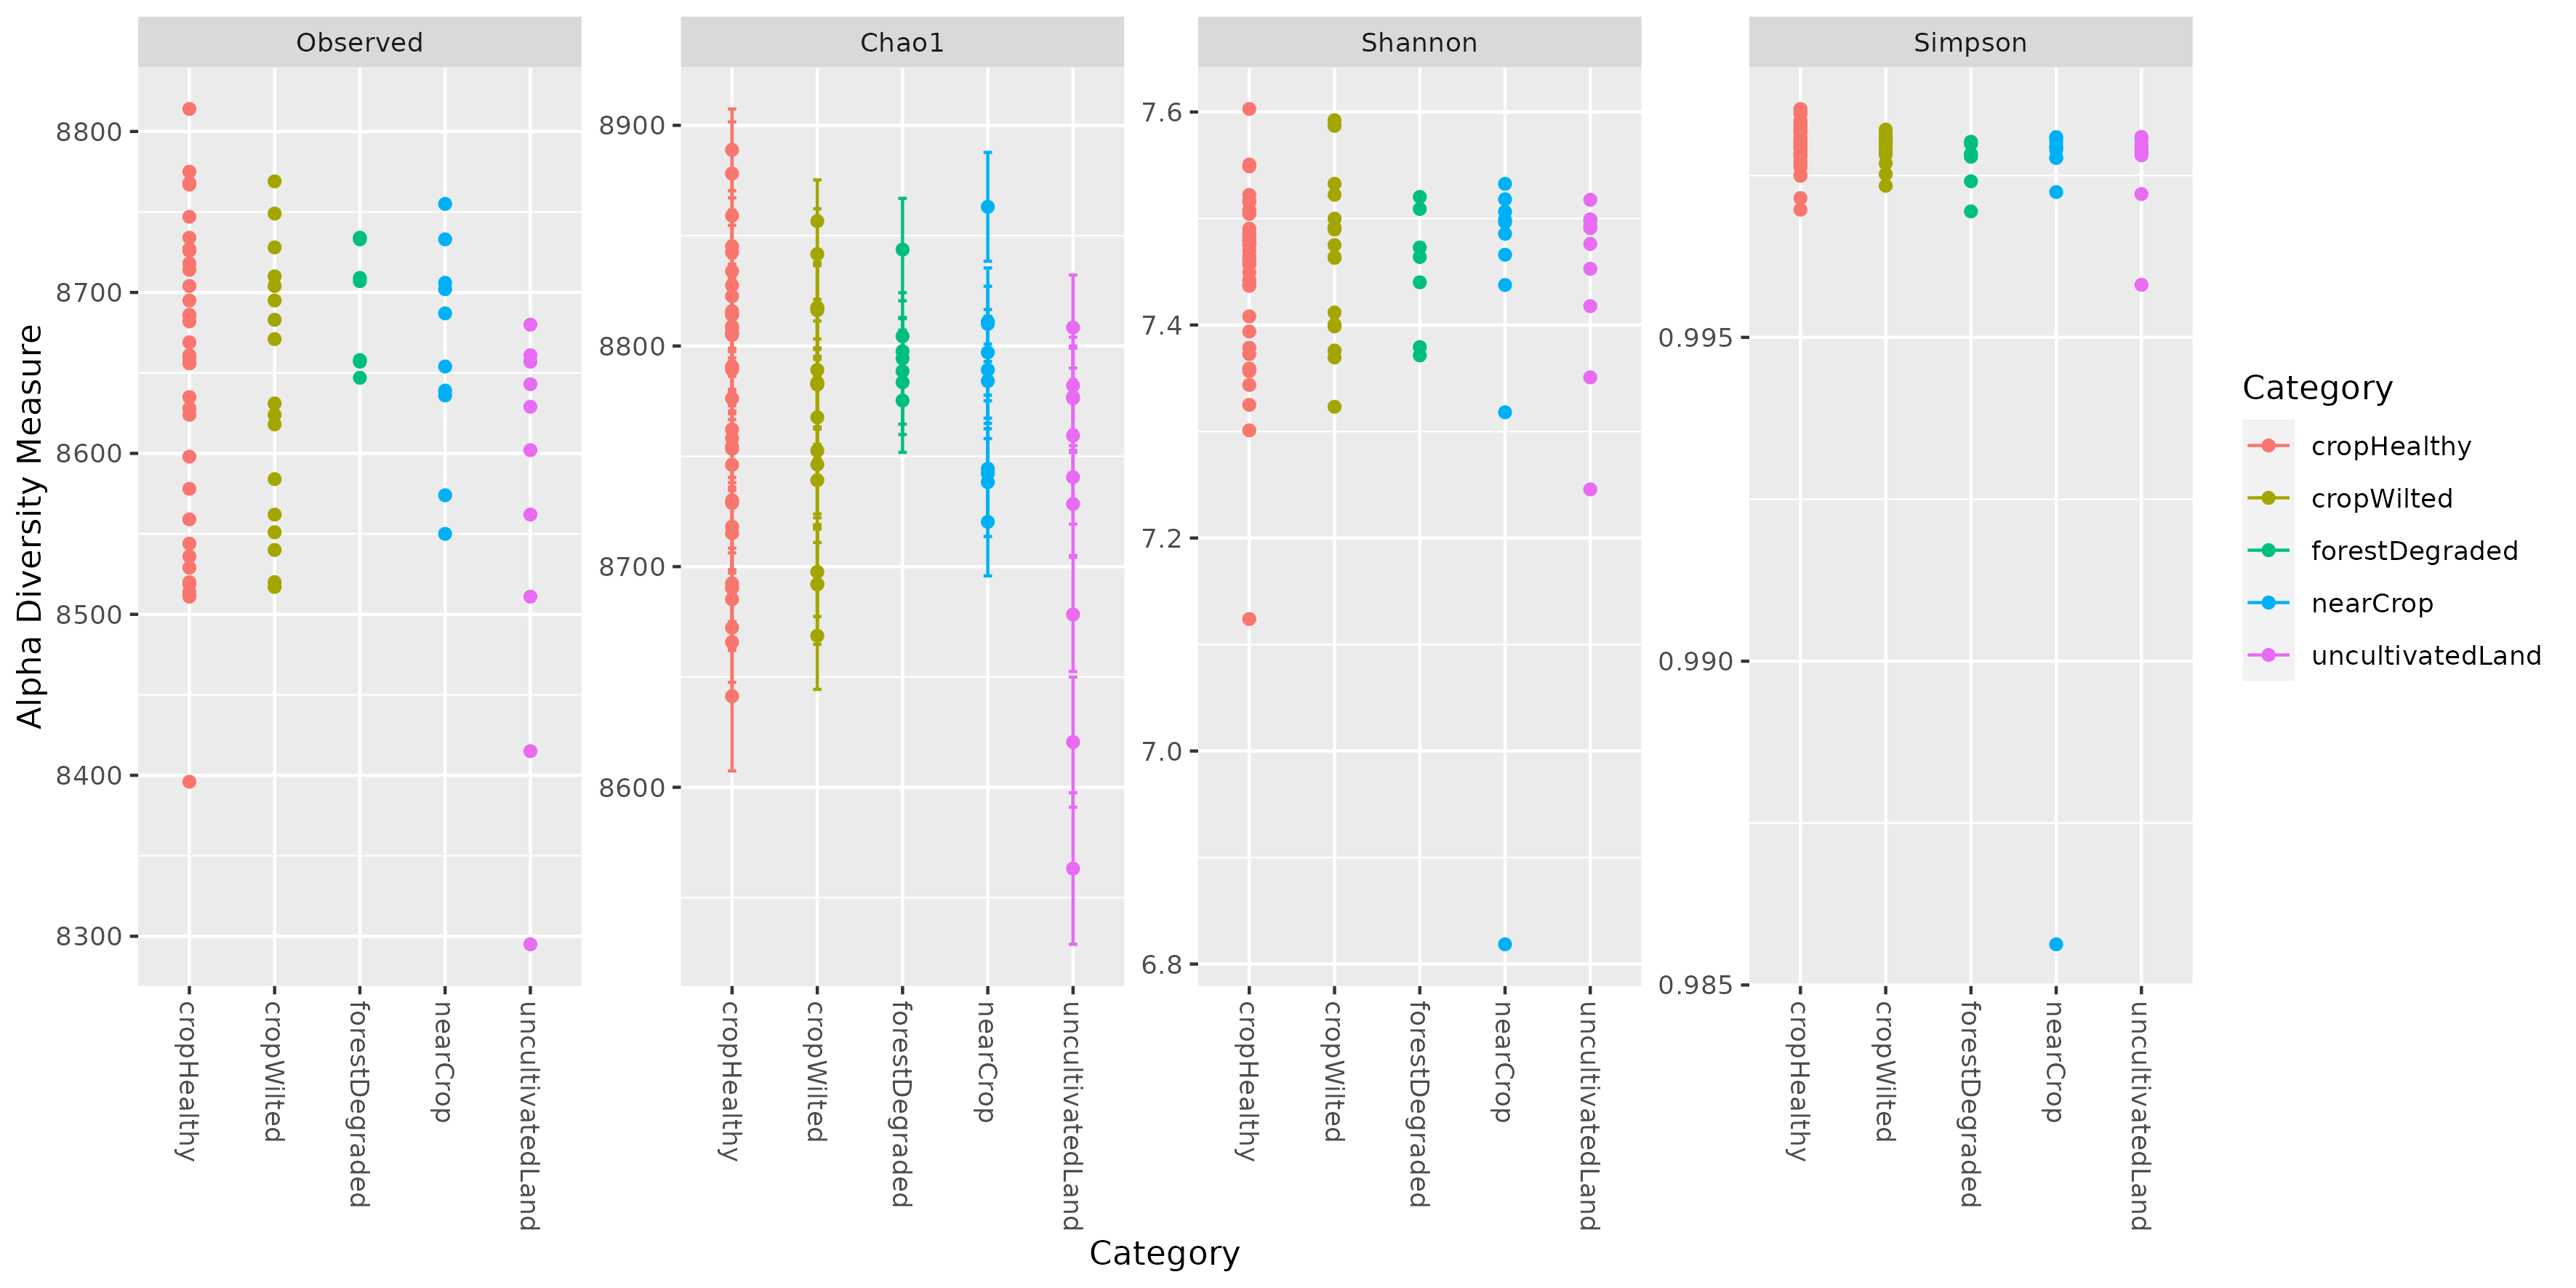
\includegraphics[width=\textwidth]{Img/cap2/AllData_Alfa_diversidad.png}
\caption{Diversidad Alfa, }
\end{figure}

\begin{figure}[!]
\centering
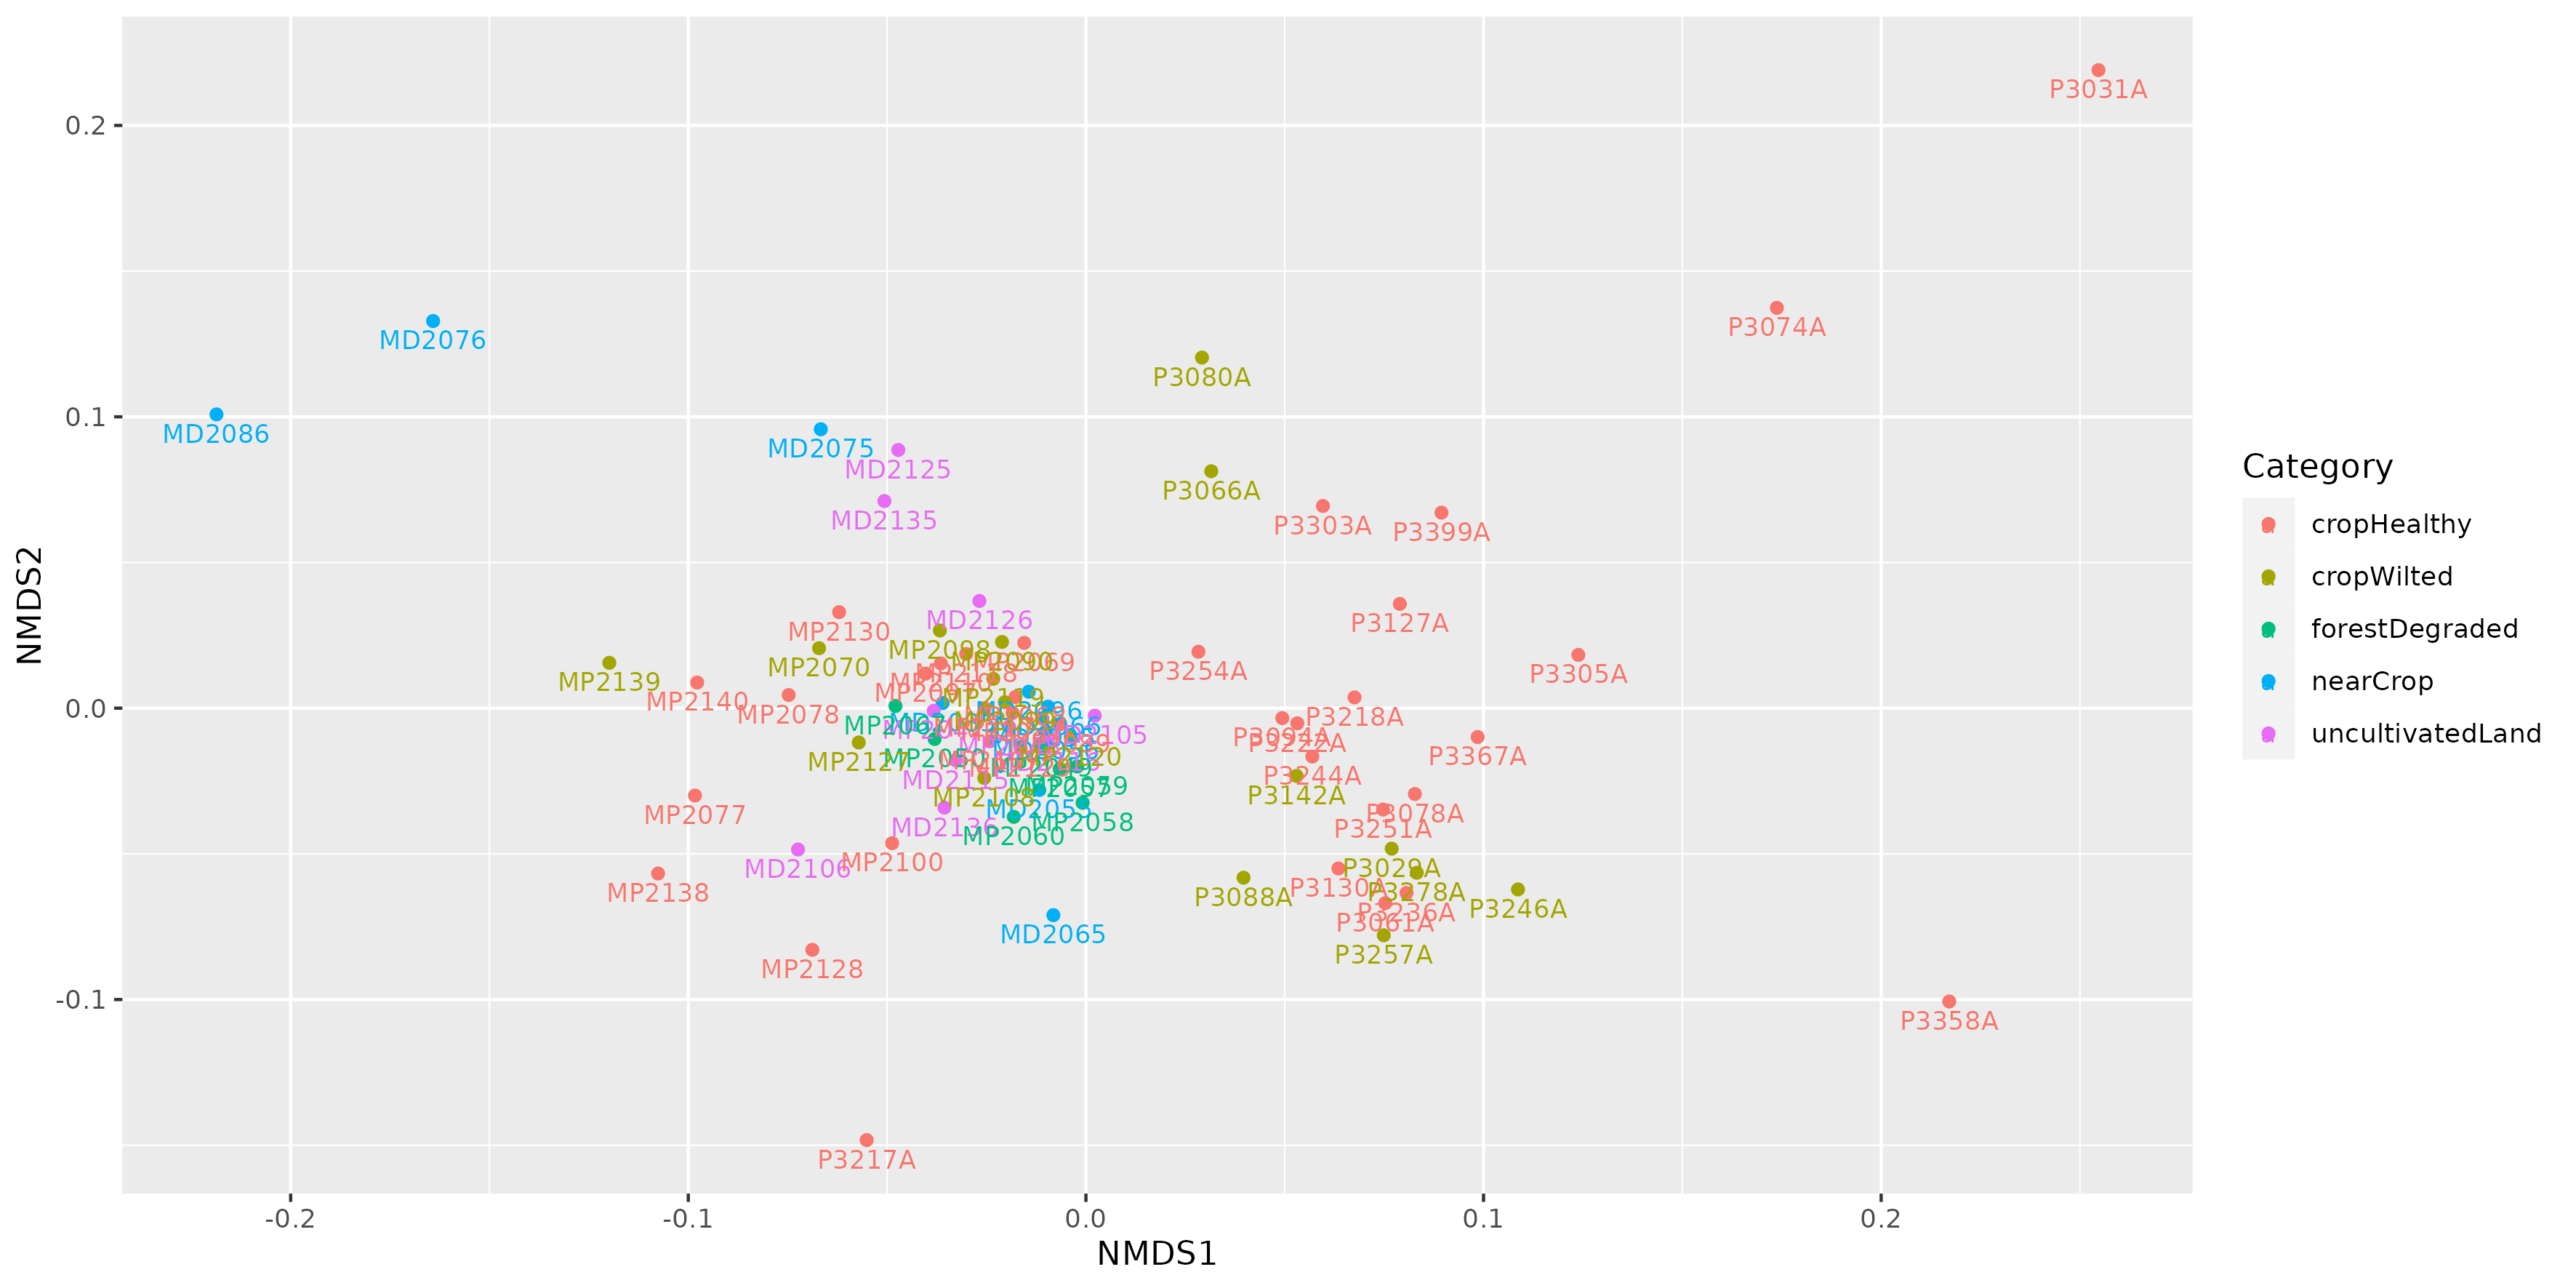
\includegraphics[width=\textwidth]{Img/cap2/AllData_Beta_diversidad.png}
\caption{Diversidad Beta, }
\end{figure}